\documentclass[fleqn,10pt]{wlscirep}
\usepackage[utf8]{inputenc}
\usepackage[T1]{fontenc}

\usepackage{url}
\usepackage{longtable}
\usepackage{booktabs}
\usepackage{seqsplit} % allows line-breaking of long \texttt{} identifiers in narrow table cells
\usepackage[per-mode=symbol]{siunitx}
\usepackage{multirow}
\usepackage{graphicx}
\usepackage{amsmath}
\usepackage{xcolor}
\usepackage{tikz}
\usetikzlibrary{positioning,arrows.meta,fit,backgrounds,calc}
\usepackage{simdgrid} % reusable SIMD lane/bit-layout primitives

\renewcommand\arraystretch{1.20}

% Long multi-panel captions overflow the caption package's single-line
% measurement ("Dimension too large"); they are never single-line anyway.
\usepackage{caption}
\captionsetup{singlelinecheck=false}

% ---------------------------------------------------------------------------
% Representation palette. ONE definition for the whole paper (DISPLAY_ITEMS.md
% section 1.1). B is achromatic on purpose: it is the foil, not a strategy.
% ---------------------------------------------------------------------------
\definecolor{reprB}{HTML}{222222} % dense bitmap (the foil; achromatic)
\definecolor{reprS}{HTML}{4477AA} % sorted array
\definecolor{reprR}{HTML}{228833} % run container
\definecolor{reprW}{HTML}{AA3377} % EWAH fill-compressed
\definecolor{reprC}{HTML}{CCBB44} % complement
\definecolor{reprRef}{HTML}{BBBBBB} % reserved: CRoaring / all-bitmap baseline

% Representation shorthands, so the symbols are typeset identically everywhere.
\newcommand{\rB}{\textsf{B}}
\newcommand{\rS}{\textsf{S}}
\newcommand{\rR}{\textsf{R}}
\newcommand{\rW}{\textsf{W}}
\newcommand{\rC}{\textsf{C}}
\newcommand{\cell}[2]{\ensuremath{#1\!\times\!#2}}

% ---------------------------------------------------------------------------
% DRAFT SCAFFOLDING. Remove \draftmode before submission.
%   \nm{...}  a number the final campaign must supply
%   \spec{...} a speculative statement pending measurement
% ---------------------------------------------------------------------------
%   \nm{...}   a number the final campaign must supply (red)
%   \spec{...} a speculative statement pending measurement (blue)
%   \prov{...} a PROVISIONAL value from the retired campaign (orange). It is
%              real data and it makes the paper readable, but every one of
%              these must be refreshed from the final campaign before
%              submission. Never let a \prov survive into a submitted draft.
\newif\ifdraftmode \draftmodetrue
\ifdraftmode
  \newcommand{\nm}[1]{\textcolor{red}{\textbf{[#1]}}}
  \newcommand{\spec}[1]{\textcolor{blue!70!black}{#1}}
  \newcommand{\prov}[1]{\textcolor{orange!85!black}{#1}}
  % \draftnote{...} is scaffolding for us, never manuscript prose: provenance
  % caveats, campaign status, internal cross-references. Vanishes entirely
  % outside draft mode, so nothing repo-internal can reach a submitted PDF.
  \newcommand{\draftnote}[1]{\textcolor{gray}{\footnotesize [#1]}}
\else
  % Outside draft mode \nm and \prov must not render. \nm{n/a} would silently
  % typeset the literal words "n/a"; \prov would ship a retired-campaign number
  % as if it were final. Both are submission-blocking and neither is visible in
  % a proofread of black-on-white output, so make the BUILD fail instead: the
  % non-draft PDF cannot exist until every slot is filled.
  \newcommand{\nm}[1]{\GenericError{}{storm: unfilled \string\nm{#1} outside
    draft mode -- the final campaign must supply this value}{}{}}
  \newcommand{\prov}[1]{\GenericError{}{storm: provisional \string\prov{#1}
    outside draft mode -- refresh from the final campaign}{}{}}
  \newcommand{\spec}[1]{#1}
  \newcommand{\draftnote}[1]{}
\fi

% ---------------------------------------------------------------------------
% Supplementary Notes. These were previously \subsection*{Supplementary Note N:
% ...} with N typed by hand in the heading AND typed again by hand at every
% citation -- two independent numberings, each silently wrong after any
% reorder. \suppnote drives both from one counter, and \refstepcounter makes a
% following \label resolvable, so the main text cites \ref and never a literal.
% ---------------------------------------------------------------------------
\newcounter{suppnote}
\newcommand{\suppnote}[1]{%
  \refstepcounter{suppnote}%
  \subsection*{Supplementary Note \thesuppnote: #1}}

% Placeholder for a figure whose data the final campaign has not yet produced.
% #1 = width fraction, #2 = what the figure will show (one line).
\newcommand{\figplaceholder}[2]{%
  \begin{center}%
  \fboxsep=10pt\fboxrule=0.6pt%
  \textcolor{red}{\fbox{\parbox{#1\linewidth}{\centering\small
  \textbf{FIGURE PLACEHOLDER}\\[3pt]#2}}}%
  \end{center}}

\title{Work avoidance for efficient sparse set algebra}

\author[1]{Marcus D. R. Klarqvist}
\affil[1]{\nm{affiliation}}

\keywords{set algebra; compressed bitmaps; adaptive representation; work
avoidance; set intersection; SIMD}

\begin{abstract}
Set algebra maps Boolean membership directly onto machine bits and underlies search indexes, graph
engines, databases and telemetry analytics. Sparse systems nevertheless often spend more time
visiting absent state than processing useful state. We use all-pairs set-intersection cardinality,
the binary Gram matrix $XX^{\mathsf T}$ underlying similarity and ranking, to develop an exact
two-scale work-avoidance architecture. Dense-bitmap execution evaluates every pair in $\Theta(m)$
work even when one row is nearly empty and the answer is usually zero. At row scale, an online selector chooses among ten
bitmap, sorted-array, run and fill-compressed representation pairings. At tile scale, coarse
positional occupancy is transposed into column postings, allowing one occupied column to generate
all row pairs it can support while the remaining pairs are proved disjoint without reading row data.
On 23 real corpora, one fixed per-tile policy was $1.48\times$--$52{,}448\times$ faster than
all-bitmap execution, and a fixed online refinement policy outperformed a query-tuned CRoaring
baseline on 22; selection remained below 1\% of runtime. In the sparse all-pairs regime, amortised
within-tile column postings were $7\times$--$5{,}700\times$ faster than unfiltered bitmap--array
evaluation. With a Jaccard threshold, element-keyed prefix postings accelerated 48 of 63
corpus--threshold configurations by $1.67\times$--$1{,}089\times$, while the gate routed the
remainder to exact scan. SIMD-throughput kernels won none of 25 asymmetric cell--shape comparisons.
All routing can begin on the first traversal from constant-size row metadata and bounded online
probes; offline optimization is optional. Set intersection thus provides an exact demonstration of
a broader sparse-systems rule: use metadata to certify absent work, amortise each decision across
many consumers and reserve throughput optimization for the work that survives.

\end{abstract}

\begin{document}

\flushbottom
\maketitle
\thispagestyle{empty}

Computing the cardinality of a set intersection, $|A \cap B|$, over a shared universe of possible
elements is a core primitive in similarity search and near-duplicate detection
\cite{bayardo2007allpairs,xiao2008ppjoin}, in chemical fingerprint screening
\cite{swamidass2007bounds,haque2011tanimoto,dalke2019chemfp}, in graph co-occurrence analysis, and
in the boolean query evaluation underneath inverted and bitmap indexes. It is a single-operation
primitive: whatever the surrounding workload, what a system pays is the cost of one operation
between two sets, and that cost is fixed by how each of the two is represented before the operation
is ever issued.

The default way to compute $|X_i \cap X_j|$ represents each set as a dense bitmap over a shared
universe of $m$ possible elements and evaluates \texttt{popcount(A AND B)} with the widest
available vector instruction. This costs $\Theta(m)$ irrespective of the cardinality of either set
or of their intersection --- every one of the $m$ bits is read and combined regardless of how many
are set --- and the underlying AND-then-popcount kernel is itself a solved problem, engineered
close to the throughput limit of the hardware \cite{mula2018popcount}. For a single pair, or for
sets that occupy a substantial fraction of the universe, this is exactly the right way to compute
the answer.

Real degree and frequency distributions are rarely uniform: a small number of categories carry
most of the mass while a long tail is rare. The canonical form of this skew --- the $i$-th most
common category scaling as $\theta/i$ --- was derived for population-genetic allele-frequency
spectra \cite{fu1995} and recurs, in shape if not in constant, in item popularity, node degree, and
category-membership counts across many other kinds of data. Under such skew, row density in the
shared-universe representation spans orders of magnitude within a single corpus, so most rows are
sparse and most pairs have at least one near-empty side --- yet the $\Theta(m)$ bitmap kernel pays
the same fixed cost regardless, spending most of that cost combining zeros against zeros.

That waste is not an anecdote about one kind of data; it is a property of the fixed cost itself, and
its size can be settled before any kernel is written. Every alternative encoding of the same set ---
a sorted array of its elements, a list of its maximal runs, a fill-compressed word stream, or any of
these applied to its complement --- is exact and interconvertible with the bitmap, and each is sized
by the set rather than by the universe. The cheapest of them is smaller than the bitmap by a factor
that grows without bound as either operand moves away from density one half, so a flat cost provably
leaves headroom at every density but the middle of the range, for a single operation as much as for
a workload of them. Assuming nothing about the data beyond its density gives a floor on that
headroom rather than an estimate of it: independently placed elements are the worst case for every
encoding whose cost depends on how a set is arranged, so real structure moves those encodings
further below the bitmap and never above it. What this paper optimizes is therefore not how fast a
kernel runs but how much of the computation is never entered. The same analysis says where that is
not possible. Around density one half no encoding is smaller than the bitmap and nothing can be
skipped; there the fixed-cost kernel is the right one, and the return comes from executing it as
fast as the hardware allows --- which is what two decades of vectorized \texttt{AND}-and-popcount
engineering already deliver \cite{mula2018popcount}. Avoid the work where it can be avoided,
accelerate it where it cannot: this paper contributes the first axis, and a cheap way of knowing
which of the two applies.

Roaring is the state of the art for exactly this problem, and it already dispatches, per
fixed-width chunk, among an array, a bitset, and a run container
\cite{chambi2016roaring,lemire2018roaring} --- the same coarse-grained skip toward a cheaper
structure that inverted-index systems such as BitFunnel apply to disjointness testing
\cite{goodwin2017bitfunnel}. It is excellent, it is deployed at scale, and this paper does not
attempt to out-engineer it at its own data structure. Its adaptivity is nonetheless fixed in
granularity and static in time: which container a chunk receives is decided by a compile-time
cardinality threshold applied to that chunk alone, chosen once at ingest for a workload built
around a single pairwise operation (Methods). That same fixed commitment prices a run container
against a bitset by iterating every run and charging for its length --- a cost a
length-independent index would remove.

All of that leaves the caller's question untouched, and a caller willing to narrow it can be given
more. If only pairs above a similarity threshold are wanted, or only operands inside a band of set
sizes, then the two cardinalities alone cap the similarity a pair can reach, so most pairs are
discarded before either operand is read \cite{swamidass2007bounds,bayardo2007allpairs} --- knowing
what is being looked for is itself a way of not doing work, and it is the cheapest one available.

Two questions follow directly. Given that popcount is a solved problem and Roaring already
dispatches on container type per chunk, is there anything left for representation choice to buy?
And if a wider representation matrix does buy something, can the choice itself be made cheaply
enough --- for one operation between two large sets, and for a batch of many small ones --- that
the saving survives the deciding?

Here we treat the representation pairing itself as the object of choice. We define a pairing
matrix of \nm{count of representation-pairing cells evaluated} cells over dense-bitmap,
sorted-array, run, and fill-compressed representations and their complements, and we measure, per
cell, which pairing is fastest across the full density range, on \nm{count of microarchitectures
tested} microarchitectures, and on \nm{count of real corpora tested} real corpora drawn from graph,
text, and tabular sources. A throughput-optimized kernel wins none of \nm{count of asymmetric
measurement points tested} asymmetric measurement points tested, while selecting among
representation pairings wins on every real corpus tested, at a selection cost that stays within a
small, budgeted fraction of runtime. We also report where the approach does not pay: a
mid-density band in which the plain bitmap kernel is, and remains, the right choice.

\section*{Results}
\label{sec:results}

We evaluated representation-pairing kernels for set-intersection cardinality. Throughout, we use
\emph{cell} to denote one representation pairing (for example $\cell{\rB}{\rS}$), \emph{variant} to
denote one implementation of a cell, and \emph{pairing matrix} to denote the full set of cells;
unless stated otherwise, every ratio is reported against a \texttt{run\_optimize}-tuned CRoaring
baseline. Figure~\ref{fig:pairing-matrix} lays out that matrix: the five representation families,
the driving variable each pairing's cost is proportional to, and the path from precomputed row
metadata through the selector to a chosen kernel.

The mechanisms reported here form a progression ordered by what a caller gives up, not by what each
costs. Choosing a representation (Fig.~\ref{fig:pairing-matrix}a--b) and consulting a zone map
(Fig.~\ref{fig:density-sweep}a) give up nothing: the question and the answer are unchanged, and
only the work changes. Prefix filtering and a size bound narrow the question instead --- only pairs
above a similarity threshold, or within a size band --- and are available only because the caller
said what they wanted; they are opt-in, never substituted for the first two, and their return is
analytic rather than measured here, reaching as little as a few per cent of pairs surviving at a
high similarity threshold (Methods, ``What makes work avoidable''; see Supplementary Note~\ref{note:threshold} and
Supplementary Fig.~\ref{fig:prefix} for the derivation and the composition rule that governs when
the two may be multiplied together). Batch amortisation leaves the contract unchanged again but
needs many operations rather than one, because what it removes is repetition rather than work.

\begin{figure}[!t]
\centering
% ===========================================================================
% Figure 1 — overview. Body only; \input inside a figure environment.
% House idiom follows the scaffold paper's fig:planes: minipage panels with
% bold letter labels, \resizebox per panel, and the two-saturation convention
% (strong fill = the lanes the panel is about, faint same-hue fill = context).
%
% Requires simdgrid.sty and the repr* colours from storm.tex.
% ===========================================================================

% Focus / context saturations, one pair per representation.
\colorlet{focB}{reprB!45}\colorlet{ctxB}{reprB!12}
\colorlet{focS}{reprS!55}\colorlet{ctxS}{reprS!14}
\colorlet{focR}{reprR!55}\colorlet{ctxR}{reprR!14}
\colorlet{focW}{reprW!55}\colorlet{ctxW}{reprW!14}
\colorlet{focC}{reprC!65}\colorlet{ctxC}{reprC!18}
\colorlet{zone}{black!18}

\tikzset{
  gridcell/.style={draw=black!55, line width=0.4pt, minimum width=16.5mm,
                   minimum height=6.6mm, inner sep=1pt, font=\scriptsize,
                   anchor=center},
  hdr/.style={font=\scriptsize\bfseries},
  flowbox/.style={draw=black!60, rounded corners=1.2pt, align=left,
                  font=\scriptsize, inner sep=3.2pt},
  flowarrow/.style={-{Latex[length=1.8mm]}, draw=black!65, line width=0.5pt},
}

% Type size. Both panels are \resizebox'd to their minipage, so the size a
% label renders at is (its point size) x (panel width / panel natural width),
% and nothing else. Measured naturals: panel a 243.8 pt at \simdcw 4.6mm,
% panel b 230.2 pt. At the previous .50/.435 split with \tiny cells, panel a's
% digits rendered 5.1 pt against panel b's 7.6 pt -- and against panel a's OWN
% 8.2 pt row labels and position ruler, which are \scriptsize.
%
% Fixed by making every glyph in panel a one size (\scriptsize, as its labels
% already were) and widening the cell so the longest token, the run record
% 12:3, still fits inside it -- cells must stay a uniform width or the strips
% stop comparing item counts, which is the panel's whole point. The two
% minipage widths are then set so both panels land at ~7 pt, matching the
% 8 pt body size of the matplotlib panels elsewhere in the paper.
\begin{minipage}[b]{.54\linewidth}
\setlength{\simdcw}{6.0mm}% local to this minipage; fits "12:3" at \scriptsize
\textbf{a}\par\vspace{0.6mm}
\resizebox{\linewidth}{!}{%
\begin{simdpicture}
  \simdstrip[font=\scriptsize\ttfamily]{5.4}{\rB}{%
    0/ctxB,1/focB,1/focB,1/focB, 0/ctxB,0/ctxB,0/ctxB,0/ctxB,%
    0/ctxB,0/ctxB,0/ctxB,0/ctxB, 1/focB,1/focB,1/focB,0/ctxB}
  \simdlabels{4.85}{0}{15}
  \node[simd note, anchor=east] at (-0.35,4.85) {position};
  \simdstrip[font=\scriptsize\ttfamily]{3.1}{\rS}{%
    1/focS,2/focS,3/focS,12/focS,13/focS,14/focS}
  \simdstrip[font=\scriptsize\ttfamily]{1.55}{\rR}{{1{:}3}/focR,{12{:}3}/focR}
  \simdstrip[font=\scriptsize\ttfamily]{0}{\rW}{L/focW,{F0}/ctxW,L/focW}
\end{simdpicture}}
\end{minipage}\hfill
% ------------------------------------------------------------------ panel b
\begin{minipage}[b]{.395\linewidth}
\textbf{b}\par\vspace{0.6mm}
\resizebox{\linewidth}{!}{%
\begin{tikzpicture}[x=1mm,y=1mm]
  % Row labels sit to the RIGHT of the grid, level with their cells, matching
  % the pair matrix in panel d.
  \foreach \c/\i in {\rB/0,\rS/1,\rR/2,\rW/3}{
    \node[hdr] at (\i*17.5,5.2) {\c};
    \node[hdr, anchor=west] at (61.8,-\i*7.1) {\c};
  }
  \node[gridcell, fill=focB]  at (0,0)      {$\Theta(m)$};
  \node[gridcell, fill=ctxS]  at (17.5,0)   {$\Theta(|S|)$};
  \node[gridcell, fill=ctxR]  at (35,0)     {$\Theta(r)$};
  \node[gridcell, fill=ctxW]  at (52.5,0)   {$\Theta(\ell{+}g)$};
  \node[gridcell, fill=ctxS]  at (17.5,-7.1){$\Theta(|A|{+}|B|)$};
  \node[gridcell, fill=ctxR]  at (35,-7.1)  {$\Theta(|S|{+}r)$};
  \node[gridcell, fill=ctxW]  at (52.5,-7.1){$\Theta(|S|{+}\ell{+}g)$};
  \node[gridcell, fill=ctxR]  at (35,-14.2) {$\Theta(r_A{+}r_B)$};
  \node[gridcell, fill=ctxW]  at (52.5,-14.2){$\Theta(r{+}\ell{+}g)$};
  \node[gridcell, fill=ctxW]  at (52.5,-21.3){$\Theta(\ell{+}g)$};
  % Lower triangle: drawn but empty. The matrix is symmetric, so these cells
  % carry no information and saying so in every one of them is noise.
  \foreach \x/\y in {0/-7.1, 0/-14.2, 17.5/-14.2, 0/-21.3, 17.5/-21.3, 35/-21.3}{
    \node[gridcell, fill=black!3, draw=black!25] at (\x,\y) {};
  }

  % The complement, shown rather than described: a dense side becomes a sparse
  % one, and re-enters the same ten cells.
  \begin{scope}[shift={(-8,-31)}]
    \foreach \bit [count=\k from 0] in {1,1,1,0,1,1,1,1,1,0,1,1,1,1,0,1}{
      \ifnum\bit=1 \def\f{focB}\else\def\f{white}\fi
      \draw[draw=black!55, line width=0.35pt, fill=\f]
        (\k*4,0) rectangle ++(4,4.4);}
    \node[hdr, anchor=east] at (-1.5,2.2) {$A$};
    \foreach \bit [count=\k from 0] in {0,0,0,1,0,0,0,0,0,1,0,0,0,0,1,0}{
      \ifnum\bit=1 \def\f{focC}\else\def\f{white}\fi
      \draw[draw=black!55, line width=0.35pt, fill=\f]
        (\k*4,-8) rectangle ++(4,4.4);}
    \node[hdr, anchor=east] at (-1.5,-5.8) {$A^{c}$};
    \draw[flowarrow] (68,2.2) -- ++(5,0) |- (68.01,-5.8);
  \end{scope}
\end{tikzpicture}}
\end{minipage}

\caption{\textbf{The object of study: equivalent encodings of one set, and the matrix of kernels
that pairing them gives.}
\textbf{a}, One set of six elements over a 16-position universe, encoded four ways. One cell is one
stored item, so a strip's length is the number of items that encoding must touch: 16 bits for $\rB$
($\Theta(m)$, whatever the set holds), six values for $\rS$ ($\Theta(|X|)$), two
$(\mathit{start}{:}\mathit{length})$ records for $\rR$ ($\Theta(r)$, whatever the runs' lengths), and
three words --- two literal and one fill --- for $\rW$ ($\Theta(\ell+g)$). Note that a cell is a bit
in $\rB$ and a word in the others, so the strips compare work, not bytes. Strong fill marks set
positions, and the position ruler applies to $\rB$ alone, the only positional encoding.
\textbf{b}, Pairing two representations gives a kernel with its own cost function. The matrix is
symmetric, so ten cells are distinct, and \emph{only} $\cell{\rB}{\rB}$ is linear in the universe
$m$; every other cell is sub-linear in it. Above density one half a side is handled through its
complement ($\rC$), shown beneath: a dense operand becomes a sparse one and re-enters the same ten
cells, with the answer recovered by inclusion--exclusion. Costs are derived in Methods.
Schematic; no measured data.}
\label{fig:pairing-matrix}
\end{figure}

\subsection*{The cost of intersection is U-shaped in density}
\label{sec:r1}

We separate the cost of intersection along density -- more precisely, each row's distance from
density one half. To determine whether the fixed cost assumed of bitmap--bitmap intersection actually holds
across the range it is assumed to hold across, and where the remaining cells beat it, we swept
density from a single set bit to a fully set universe and measured every one of
\nm{count of pairing cells swept in the density sweep} cells at each point. Both sides were swept at
matched density with the universe pinned at \nm{universe size held fixed across the density sweep,
in bits} bits, so that cache residency -- \nm{cache level the density sweep is resident in, e.g.\
L2} throughout -- stayed constant along the axis instead of confounding it. The sweep in
Fig.~\ref{fig:density-sweep} covers the uniform spectrum; the $1/i$ spectrum, exercised identically,
is reported in Supplementary Fig.~\nm{number of the supplementary figure carrying the 1/i density
sweep}.

Bitmap--bitmap cost was flat across the swept range -- \nm{$\cell{\rB}{\rB}$ cost, ns per pair, range
across the density sweep} at the cache residency stated above, spanning
\nm{order-of-magnitude span of the density sweep} orders of magnitude of density -- which turns the
fixed-cost premise underlying the standard approach from an argument into a measurement. Against
that flat line, the best cell at the sparsest density point beat $\cell{\rB}{\rB}$ by
\nm{best-cell speedup over $\cell{\rB}{\rB}$ at the sparsest density point}, and the advantage grew
with universe size.

The two curves crossed at approximately \nm{crossover density, order of magnitude, stated as an
approximate value} -- an approximate value, since the exact crossover moves under re-measurement even
though its existence does not. Near density one, the curve turned again: a row that is almost
entirely set has a complement that is almost entirely empty, and \spec{we expect a complement-based
cell, $\cell{\rC}{\rB}$ or $\cell{\rC}{\rC}$, to win the dense tail as a designed strategy, beating the
margin achieved when $\cell{\rR}{\rR}$ wins only incidentally}, beating $\cell{\rB}{\rB}$
by \nm{dense-tail win ratio over $\cell{\rB}{\rB}$ at the densest measured point}. The result is a U,
not a monotonic curve, and it corrects the framing this project began with: the operative variable is
not sparsity but distance from density one half, since a row that is 99.99\% set is exactly as
compressible as one that is 0.01\% set (Fig.~\ref{fig:density-sweep}).

\begin{figure}[!p]
\centering
\footnotesize
\textbf{a}\par\vspace{0.4mm}
% Zone-map schematic (was Fig. 1c)
% Extracted from the former Fig. 1; rendered as a panel of its own figure.
\centering
% ===========================================================================
% Figure 1 — overview. Body only; \input inside a figure environment.
% House idiom follows the scaffold paper's fig:planes: minipage panels with
% bold letter labels, \resizebox per panel, and the two-saturation convention
% (strong fill = the lanes the panel is about, faint same-hue fill = context).
%
% Requires simdgrid.sty and the repr* colours from storm.tex.
% ===========================================================================

% Focus / context saturations, one pair per representation.
\colorlet{focB}{reprB!45}\colorlet{ctxB}{reprB!12}
\colorlet{focS}{reprS!55}\colorlet{ctxS}{reprS!14}
\colorlet{focR}{reprR!55}\colorlet{ctxR}{reprR!14}
\colorlet{focW}{reprW!55}\colorlet{ctxW}{reprW!14}
\colorlet{focC}{reprC!65}\colorlet{ctxC}{reprC!18}
\colorlet{zone}{black!18}

\tikzset{
  gridcell/.style={draw=black!55, line width=0.4pt, minimum width=16.5mm,
                   minimum height=6.6mm, inner sep=1pt, font=\scriptsize,
                   anchor=center},
  hdr/.style={font=\scriptsize\bfseries},
  flowbox/.style={draw=black!60, rounded corners=1.2pt, align=left,
                  font=\scriptsize, inner sep=3.2pt},
  flowarrow/.style={-{Latex[length=1.8mm]}, draw=black!65, line width=0.5pt},
}

% ------------------------------------------------------------------ panel c
\resizebox{.506\linewidth}{!}{%
\begin{simdpicture}
  % One verdict per bin, carried as a colour down the whole column, so the
  % reader can trace a bin top-to-bottom. Colour here is the SAME reserved
  % cost/saving axis used in the matplotlib panels of this figure and of
  % Supplementary Fig. S1, and it means the same thing in all of them:
  %   workc  = there is data here, so this bin costs work
  %   avoidc = nothing here, so the work is skipped
  % It formerly ran green-for-occupied against red-for-empty, which inverted
  % the sense of green between this panel and panel e (where green marked work
  % NEVER done) and spent R's representation hue on a non-representation
  % meaning. Neither is true now.
  %
  % Colour is never the only encoding: the 0/1 digits, the tick/cross glyphs,
  % the fill/text-contrast pairing (white on the dark accent, black on the
  % light one) and the dashed bin rules each carry the verdict on their own,
  % so the panel reads in greyscale.
  \definecolor{workc}{HTML}{EE6677}
  \definecolor{avoidc}{HTML}{66CCEE}
  \colorlet{visitc}{workc}
  \colorlet{skipc}{avoidc}

  % Each row is coloured by ITS OWN occupancy, so the AND row reads as the
  % product of the two above it: work AND work = work, work AND skip = skip.
  % Bin 1 is the instructive case -- B occupies it, A does not, so occ_B is
  % red, occ_A is cyan, and the pair skips the bin.
  %
  % Type size: cells were \tiny against \scriptsize row labels inside one
  % picture, so the digits rendered about 3.6 pt on the page. Both are
  % \scriptsize now and the picture is scaled to render at roughly 8 pt, the
  % same body size as the matplotlib panels beneath it.
  \foreach \bin/\ca/\ta/\cb/\tb/\cn/\tn/\abits/\bbits/\oa/\ob/\an in {%
      0/workc/white/workc/white/workc/white/{0,1,0,0}/{0,0,1,0}/1/1/1,
      1/avoidc/black/workc/white/avoidc/black/{0,0,0,0}/{0,0,1,0}/0/1/0,
      2/avoidc/black/avoidc/black/avoidc/black/{0,0,0,0}/{0,0,0,0}/0/0/0,
      3/workc/white/workc/white/workc/white/{0,1,0,0}/{0,0,1,0}/1/1/1}{%
    % Operand rows: light tint of that row's own verdict, set bits at full.
    % Text colour tracks the fill so every digit stays legible on both accents
    % -- white on the mid-tone red, black on the light cyan.
    \foreach \bit [count=\k from 0] in \abits {%
      \ifnum\bit=1\relax
        \node[simd cell, fill=\ca, text=\ta, font=\scriptsize\ttfamily]
          at (\bin*4+\k,2) {1};
      \else \node[simd cell, fill=\ca!15, text=black!60, font=\scriptsize\ttfamily]
          at (\bin*4+\k,2) {0};\fi}
    \foreach \bit [count=\k from 0] in \bbits {%
      \ifnum\bit=1\relax
        \node[simd cell, fill=\cb, text=\tb, font=\scriptsize\ttfamily]
          at (\bin*4+\k,0) {1};
      \else \node[simd cell, fill=\cb!15, text=black!60, font=\scriptsize\ttfamily]
          at (\bin*4+\k,0) {0};\fi}
    % summary rows, each in its own row's colour; the AND row is the product
    \node[simd cell, fill=\ca, text=\ta, font=\scriptsize\ttfamily,
          minimum width=4\simdcw] at (\bin*4,-1.7) {\oa};
    \node[simd cell, fill=\cb, text=\tb, font=\scriptsize\ttfamily,
          minimum width=4\simdcw] at (\bin*4,-3.1) {\ob};
    % the AND itself -- this is the mechanism, kept as bits
    \node[simd cell, fill=\cn, text=\tn, font=\scriptsize\ttfamily,
          minimum width=4\simdcw, line width=0.8pt, draw=black!70]
      at (\bin*4,-4.5) {\an};
    % and its readout, as a glyph. Glyphs are drawn dark rather than in the
    % accent itself, so they stay the panel's most legible encoding.
    \node[simd cell, fill=\cn!12, minimum width=4\simdcw,
          draw=\cn, line width=0.7pt] at (\bin*4,-5.9) {};
    \ifnum\an=1\relax
      \draw[line width=1.1pt, draw=workc!65!black, line cap=round, line join=round]
        (\bin*4+1.62,-5.40) -- (\bin*4+1.86,-5.68) -- (\bin*4+2.40,-5.08);
    \else
      \draw[line width=1.1pt, draw=avoidc!55!black, line cap=round]
        (\bin*4+1.72,-5.68) -- (\bin*4+2.28,-5.12)
        (\bin*4+1.72,-5.12) -- (\bin*4+2.28,-5.68);
    \fi
  }

  \node[simd label] at (-0.35,2.5) {$A$};
  \node[simd label] at (-0.35,0.5) {$B$};
  \node[simd label] at (-0.35,-1.2) {$\mathrm{occ}_A$};
  \node[simd label] at (-0.35,-2.6) {$\mathrm{occ}_B$};
  \node[simd label] at (-0.35,-4.0) {$\mathrm{occ}_A \wedge \mathrm{occ}_B$};
  \node[simd label] at (-0.35,-5.4) {visit?};
  \foreach \b in {0,4,8,12,16}{
    \draw[black!45, dashed, line width=0.35pt] (\b,-6.1) -- (\b,3.35);}
  \simdbrace{0}{16}{-6.5}{popcount $=2$: visit bins 0 and 3, skip half the universe}
\end{simdpicture}}


\vspace{0.4mm}
\par\vspace{1.0mm}
% The canvas is generated at exactly \textwidth, so it is included at full
% width and never scaled: at the previous .75 it rendered its 8 pt body text
% at 4.5 pt and its annotations below 4 pt.
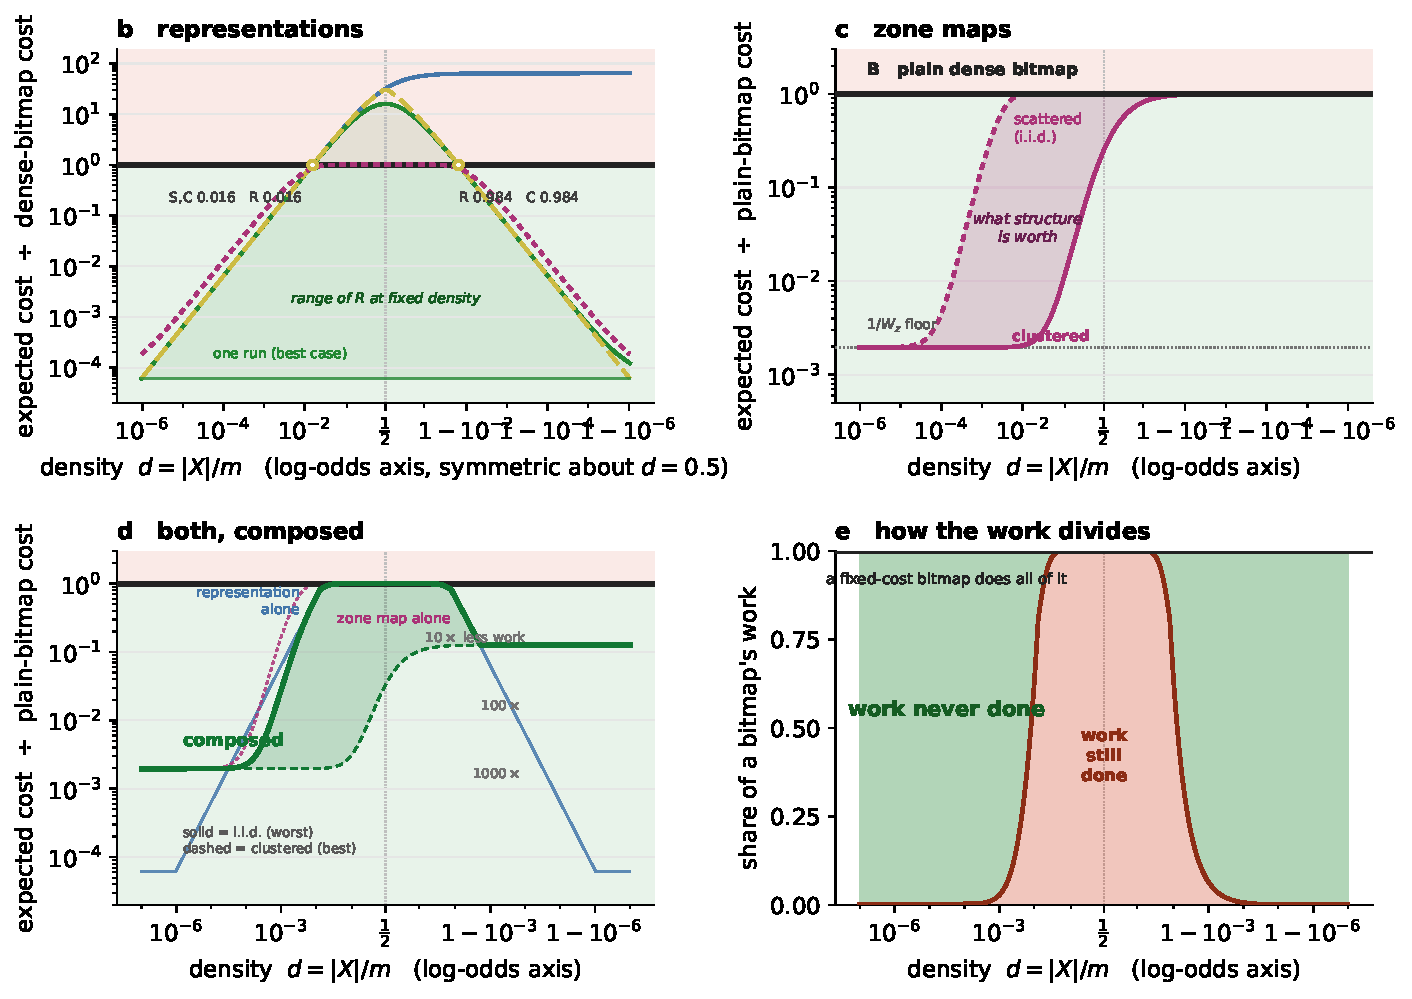
\includegraphics[width=\linewidth]{figures/fig2_expectations}
\caption{\textbf{What a fixed cost leaves on the table, analytically.} Derived, not measured; every
panel models \emph{work} rather than time. Reading key: hue names a representation, so mechanisms
are grey and separated by line style; red marks work still done, cyan work avoided, and grey shading
the region dearer than a plain bitmap.
\textbf{a}, A zone map within one pair. Each bin carries one bit recording whether that operand
holds anything in it, and $\mathrm{occ}_A \wedge \mathrm{occ}_B$ is the AND of the two summaries.
Follow bin~1: $B$ occupies it and $A$ does not, so the pair skips the bin even though one side holds
data there. The popcount of the AND is the \emph{exact} number of bins to visit, and a popcount of
zero proves the operands disjoint without reading either. Digits and glyphs repeat every verdict, so
the panel reads without colour.
\textbf{b}, Expected cost of each representation for a uniformly random set, as a multiple of the
dense-bitmap cost, on a log-odds density axis. Every cost is proportional to the universe $m$, so
this panel is scale-invariant and the crossovers are universal constants: open circles at
$d = 1/w = 0.0156$ for $\rS$ and $\rC$, $0.0159$ for $\rR$, and their complements. The bitmap is the
line at $1$. Shading marks the range of $\rR$ at fixed density --- one run at best, the i.i.d. value
at worst --- which is the deviation the method exploits.
\textbf{c}, The same for a zone map. Arrangement, not density, sets the share of bins an operand
occupies: at $d = 0.01$ and $W_z = 512$ the scattered and clustered extremes differ by
$482\times$, so the i.i.d. curve floors what a summary is worth.
\textbf{d}, The two composed. Filtering concentrates density, so the representation used inside a
surviving bin is the one for that bin's local density. Clustered, the composition costs $0.195\%$ of
a bitmap across the sparse range at $W_z = 512$, rising to $12.7\%$ only in the dense half; the knee
sits at $d = 1/8$ for every bin width.
\textbf{e}, The same as a division of labour: the share of a bitmap's work never done against the
share still done, taking the best of the four options at each density. $99.8\%$ is never done
at $d = 10^{-4}$; the waist about $d = \tfrac12$ is where a bitmap is the right kernel.
Measurements on real corpora appear on these axes in Supplementary Fig.~\nm{number}.}
\label{fig:density-sweep}
\end{figure}

Each mechanism above is a bet that the data deviates from randomness, and the size of the win at the
sparse extreme, the location of the crossover, and the two-sided condition under which a zone map is
worth consulting at all follow from a closed-form counting argument against the least favourable
(independent-placement) arrangement of elements, given in full in Supplementary Note~\ref{note:zonemap}. Inside the
band where nothing beats $\cell{\rB}{\rB}$ (Fig.~\ref{fig:density-sweep}d), no encoding is smaller
than the bitmap and no bin is empty, so the return there comes from throughput rather than
avoidance --- the axis the vectorized \texttt{AND}-and-popcount literature has already carried a
long way \cite{mula2018popcount}.

\subsection*{The winning representation pairing migrates across real corpora}
\label{sec:r2}

The sweep above varies density by construction, and a generator can always be
suspected of encoding exactly the structure its own kernels are built to exploit. We therefore
repeated the central comparison on corpora of independent provenance: the twelve corpora CRoaring's
own benchmark harness runs by default \cite{chambi2016roaring,lemire2018roaring}, together with
\prov{five} larger modern graphs, for \prov{17} corpora spanning \prov{$7.89\times10^{-7}$ to
$1.73\times10^{-1}$} in density and \prov{$1.995\times10^{5}$ to $3.697\times10^{7}$} bits in universe
size (full provenance, and the further corpora scored only against an all-bitmap baseline, in
Supplementary Table~\ref{tab:corpus-inventory}, Supplementary Note~\ref{note:corpora}). Every corpus is scored against
the same \texttt{run\_optimize()}-tuned CRoaring baseline used throughout Results, so this comparison
is continuous with the synthetic sweeps above rather than separate from them.

Table~\ref{tab:corpora} reports, for every corpus, universe size and density, the pairing cell that
won under best-cell (oracle) selection, and the ratio against tuned CRoaring and against an
all-bitmap baseline. Both ratios are oracle: hindsight choice of representation pairing with
no selection cost charged, not the deployed selector run end to end (Methods, ``Selection policies:
per-pair, per-tile, and probe-and-commit''); an end-to-end evaluation of the deployed selector is
not part of this study.
Storm's best cell beat tuned CRoaring on \prov{17 of 17} corpora tested, ratio range
\prov{$1.12\times$ to $16.06\times$}, median \prov{$\approx 6.1\times$}, excluding
\texttt{uscensus2000} and \texttt{dimension\_033}, whose repeats could not be pinned to the precision
shown (Methods, ``Statistics and aggregation''; their density and winning cell are unaffected and
still reported).

\begin{table}[!t]
\scriptsize
\setlength{\tabcolsep}{2.2pt}
\renewcommand\arraystretch{1.05}
\centering
\caption{\textbf{The winning representation pairing migrates with corpus density.} \prov{14 of 23}
real corpora (Methods, ``Corpora, provenance and loaders''; full inventory in Supplementary
Table~\ref{tab:corpus-inventory}), grouped by density band and chosen to span every domain and both
speedup extremes; the remaining \prov{9} corpora are summarised in the final row.
\texttt{1KGP3 chr20} (haplotype-major) is included in the Mixed band as this paper's own stated
counterexample and is not omitted for being unflattering. Both ratio columns are oracle:
best-cell selection with hindsight, no selection cost charged, not the deployed end-to-end selector
(Methods, ``Selection policies: per-pair, per-tile, and probe-and-commit''). ``vs.\ CRoaring'' is
against a \texttt{run\_optimize()}-tuned baseline
\cite{chambi2016roaring,lemire2018roaring}. ``vs.\
all-bitmap'' is context only, from a separate benchmark, and the two ratio columns in one row need
not come from the same measurement. Winning cell in bold, and the vs.\ CRoaring ratio is bold on the same rows, marking the
rows for which a confirmed oracle result exists; ---, not applicable. $^\dagger$ ratio not
quotable to the precision shown (Methods, ``Statistics and aggregation''); density and winning cell
are corpus properties and unaffected. $^\ddagger$ vs.\ all-bitmap only; no CRoaring value exists for
this row. $^\S$ scoping corpus, not part of the 23-corpus set; a ratio below $1.0\times$ is a genuine
loss for selection at this density and layout. \draftnote{All values provisional, pending the final
measurement campaign.}}
\label{tab:corpora}
\begin{tabular}{@{}c l l r r l r r@{}}
\toprule
& Corpus & Domain & {Universe $m$ (bits)} & {Density} & Winning cell & {vs.\ CRoaring (oracle, $\times$)} & {vs.\ all-bitmap ($\times$)} \\
\midrule
\multirow{7}{*}{Sparse}
& \texttt{enwiki-categorylinks} & IR      & {1.30e8} & {7.89e-7} & {\nm{cell}} & {\nm{n/a}} & {\prov{1083}$^\ddagger$} \\
& \texttt{uscensus2000}$^\dagger$ & census & {3.70e7} & {8.09e-7} & {\prov{B$\times$S}$^\dagger$} & {$^\dagger$} & {$^\dagger$} \\
& \texttt{dbpedia-link}         & graph   & {1.83e7} & {1.63e-6} & {\nm{cell}} & {\nm{n/a}} & {\prov{311}$^\ddagger$} \\
& \texttt{as-skitter}           & graph   & {1.70e6} & {9.08e-6} & \textbf{\prov{B$\times$S}} & {\textbf{\prov{4.02}}} & {\prov{756}} \\
& \texttt{wiki-Talk}            & graph   & {2.39e6} & {2.17e-5} & \textbf{\prov{B$\times$S}} & {\textbf{\prov{8.80}}} & {\prov{910}} \\
& \texttt{gnomad\_chr21\_exomes\_af1e-3} & genomics & {1.46e6} & {1.93e-5} & {\nm{cell}} & {\nm{n/a}} & {\prov{222}$^\ddagger$} \\
& \texttt{dimension\_008}       & druid   & {3.87e6} & {8.98e-5} & \textbf{\prov{R$\times$R}} & {\textbf{\prov{1.73}}} & {\prov{2846}} \\
\midrule
\multirow{5}{*}{Mixed}
& \texttt{usher\_sarscov2}      & genomics & {8.45e6} & {1.87e-3} & {\nm{cell}} & {\nm{n/a}} & {\prov{121}$^\ddagger$} \\
& \texttt{wikileaks-noquotes}   & text    & {1.35e6} & {1.02e-3} & \textbf{\prov{B$\times$B}} & {\textbf{\prov{6.79}}} & {\prov{67}} \\
& \texttt{census1881}           & census  & {4.28e6} & {1.17e-3} & \textbf{\prov{B$\times$B}} & {\textbf{\prov{16.06}}} & {\prov{151}} \\
& \texttt{dimension\_033}$^\dagger$ & druid & {3.87e6} & {5.78e-3} & {\prov{B$\times$R}$^\dagger$} & {$^\dagger$} & {$^\dagger$} \\
& \texttt{1KGP3 chr20} (hap.-major)$^\S$ & genomics & {1.05e6} & {3.1e-2} & \textbf{\prov{B$\times$B}} & {\nm{n/a}} & {\prov{0.93}$^\S$} \\
\midrule
\multirow{3}{*}{Dense}
& \texttt{weather\_sept\_85}    & sensor  & {1.02e6} & {6.34e-2} & \textbf{\prov{B$\times$B}} & {\textbf{\prov{15.02}}} & {\prov{2}} \\
& \texttt{msprime\_10k}         & genomics-sim & {2.00e4} & {9.4e-2} & {\nm{cell}} & {\nm{n/a}} & {\prov{2}$^\ddagger$} \\
& \texttt{census-income}        & census  & {2.00e5} & {1.73e-1} & \textbf{\prov{B$\times$B}} & {\textbf{\prov{13.11}}} & {\prov{1}} \\
\addlinespace
& \multicolumn{2}{l}{remaining \prov{9} corpora (Supplementary Table~\ref{tab:corpus-inventory})} & {---} & {\prov{4.15e-6--7.9e-2}} & varies & {\prov{1.12--6.07}} & {\prov{3--523}} \\
\bottomrule
\end{tabular}
\end{table}

More informative than either ratio is which cell wins where. Across the corpus set, \prov{$\cell{\rB}{\rB}$
wins 10, $\cell{\rB}{\rS}$ wins 3, $\cell{\rB}{\rR}$ wins 2, $\cell{\rS}{\rS}$ wins 1, and
$\cell{\rR}{\rR}$ wins 1}: no cell accounts for a plurality, let alone all of the corpora. Had one
cell dominated, the pairing matrix would have had nothing left to select among; instead the winner
tracks each corpus's density, as the density sweep above predicts. \spec{The sparse end is won by
array- and rank-based cells, the dense end by $\cell{\rB}{\rB}$, and clustered corpora by run-based
cells -- the same three regimes the U-shaped curve predicts, now read off independently sourced data
rather than a generator.} The fill-compressed cell, $\cell{\rW}{\rW}$, underperforms tuned CRoaring on
\prov{16 of 17} corpora, \spec{the clearest real-data instance of the cost of choosing wrong that this
paper argues throughout}. Taken together, the migration and the histogram, not any single ratio, are
the result reported here: a map of which representation is correct for which corpus, read directly
off data whose structure this project did not generate.

\subsection*{A storage-priced container rule leaves query cost unclaimed}
\label{sec:r3}

Several corpora at moderate-to-high global density -- \prov{$1.2\times10^{-3}$ to $1.7\times10^{-1}$}
-- lose to Storm by more than an equally dense popcount workload should explain
(Table~\ref{tab:corpora}), so we asked whether CRoaring's own container choice, not only Storm's
kernels, accounts for the gap. We used CRoaring's own introspection API to census the array, bitset
and run containers a \texttt{run\_optimize()}-tuned bitmap settles on, counted after tuning so the
census reflects how the library is actually deployed (Methods, ``Container census'').

\begin{table}[!t]
\footnotesize
\setlength{\tabcolsep}{6pt}
\renewcommand\arraystretch{1.05}
\centering
\caption{\textbf{Roaring's fixed per-chunk threshold is tested against the wrong statistic.}
Container composition of a \texttt{run\_optimize()}-tuned CRoaring bitmap
\cite{chambi2016roaring,lemire2018roaring}, counted after tuning (Methods, ``Container census''), for
\prov{four} corpora spanning the density range of Table~\ref{tab:corpora}, including
\texttt{uscensus2000} at extreme sparsity to check whether the same array-container plurality
persists there too (it does). Roaring assigns a bitset
container to a $2^{16}$-bit chunk only when that chunk's own cardinality exceeds a fixed compile-time
constant \prov{(4096; vendor source, not measured here)} --- a per-chunk statistic, not the corpus's
global density --- so a corpus that is dense in aggregate can receive almost no bitset containers.
Total chunks sums the three container counts. Bold marks the plurality container type per
row; all four rows are plurality-array. \draftnote{All values provisional, pending the final
measurement campaign.}}
\label{tab:census}
\begin{tabular}{@{}l r r r r r@{}}
\toprule
Corpus & {Global density} & {Array containers} & {Bitset containers} & {Run containers} & {Total chunks} \\
\midrule
\texttt{uscensus2000}   & {\prov{8.1e-7}} & {\textbf{\prov{2{,}219}}} & {\prov{0}} & {\prov{2}} & {\prov{2{,}221}} \\
\texttt{census1881}     & {\prov{1.2e-3}} & {\textbf{\prov{1{,}332}}} & {\prov{0}} & {\prov{132}} & {\prov{1{,}464}} \\
\texttt{weather\_sept\_85} & {\prov{6.3e-2}} & {\textbf{\prov{2{,}274}}} & {\prov{561}} & {\prov{21}} & {\prov{2{,}856}} \\
\texttt{census-income}  & {\prov{1.7e-1}} & {\textbf{\prov{553}}} & {\prov{180}} & {\prov{35}} & {\prov{768}} \\
\bottomrule
\end{tabular}
\end{table}

On \texttt{census1881} at \prov{$1.2\times10^{-3}$} global density, the tuned bitmap holds
\prov{1{,}332} array containers against \prov{\textbf{0}} bitset and \prov{132} run containers, out of
\prov{1{,}464} chunks (Table~\ref{tab:census}): essentially no chunk ever crosses the threshold,
despite the corpus being dense by any global measure. The threshold tests a per-chunk statistic -- a
chunk's own cardinality -- rather than the corpus's global density, so mass can spread across enough
chunks that every individual chunk stays under threshold while global density reaches \prov{6.3\%}
(\texttt{weather\_sept\_85}) or \prov{17.3\%} (\texttt{census-income}), and CRoaring runs array merges
where a bitmap popcount would be strictly cheaper. This is not evidence of poor engineering; it is
evidence that a threshold fixed once, at ingest, for a workload built around a single pairwise
operation cannot be correct at every global density a corpus is later evaluated at -- the
fixed-granularity limitation this paper's opening names.

That mechanism predicts that no single fixed cardinality threshold can be correct across the density
axis, the same argument this paper makes generally, now applied to the incumbent. The constant itself
points at why: \prov{4096} is where a stored array and a bitset consume equal memory -- a size
crossover, chosen for storage rather than for compute -- while the compute crossover for a
count-only AND on this host sits at cardinality \prov{64--128}, so the stock threshold is
\prov{30--60$\times$} too high for this workload. We tested the prediction directly: promoting array
containers above cardinality \prov{$\approx$64} to bitsets after
\texttt{run\_optimize()} -- a twenty-line change to CRoaring -- removes most of the dense-corpus
advantage above (\texttt{census1881} \prov{$13.40\times \to 0.59\times$}; \texttt{census-income}
\prov{$10.65\times \to 1.88\times$}; \texttt{wikileaks-noquotes} \prov{$5.15\times \to 3.67\times$}),
while several sparse corpora are unaffected or improve (\texttt{as-skitter}
\prov{$3.35\times \to 3.23\times$}; \texttt{dbpedia-link} \prov{$2.44\times \to 2.79\times$};
\texttt{uscensus2000} \prov{$2.27\times \to 2.76\times$}), for a net \prov{$\approx19.5\times$} gain on
dense corpora against a \prov{$0.6$--$0.8\times$} loss on sparse ones. Neither \prov{4096} nor
\prov{64} is correct at both ends of the density axis: this is the paper's own thesis demonstrated
inside the incumbent, and it reframes the finding above from a defect in Roaring to a case for
adaptive selection in Roaring, for the same reason Storm needs it.

What this withdraws is a kernel-level advantage -- Storm's dense cells beating CRoaring's dense cells
-- which was never the paper's contribution. With the avoidance mechanisms above (zone maps, gating,
the size bound) applied on top of either CRoaring configuration, representation selection still wins,
because those mechanisms sit above whichever kernel is underneath them and compose with a better one
exactly as they compose with a worse one. The array-promotion fix itself is offered upstream rather
than scored against: it is a twenty-line change to a widely deployed library, not a criticism of
its engineering. \draftnote{Re-derive every CRoaring column in
Table~\ref{tab:corpora} against the array-promotion baseline before submission, and report both
baselines throughout.}


% sections/results_b.tex
% Results R4-R6. Continues \section{Results} opened in sections/results_a.tex;
% do not re-issue \section{Results} here. results/ is empty and the campaign
% is re-running -- every quantity below is \nm{...}; every speculative
% sentence is wrapped in \spec{...}. See NARRATIVE.md \S12 for the Table 1
% restructuring this file implements (deployed end-to-end headline column,
% best-cell oracle as a labelled upper bound, gap = regret).

\subsection*{The winning representation pairing migrates across real corpora}
\label{sec:r4}

The sweeps in the preceding subsections vary density and working-set size by
construction, and a generator can always be suspected of encoding exactly the
structure its own kernels are built to exploit. We therefore repeated the
central comparison on corpora with independent provenance: the twelve corpora
CRoaring's own benchmark harness runs by default \cite{chambi2016roaring,lemire2018roaring},
together with \prov{five} larger modern graphs, for \prov{17} corpora spanning
\prov{$7.89\times10^{-7}$ to $1.73\times10^{-1}$} in density and
\prov{$1.995\times10^{5}$ to $3.697\times10^{7}$} bits in universe size
(Supplementary Table~\ref{tab:corpus-inventory} lists the provenance of every
corpus, including the further corpora scored only against an all-bitmap
baseline, never against CRoaring). Every corpus in this seventeen-corpus set
is scored against the same \texttt{run\_optimize()}-tuned CRoaring baseline
used throughout Results, so this comparison is continuous with, not separate
from, the synthetic sweeps above.

Table~\ref{tab:corpora} reports, for every corpus, its universe size and
density, the pairing cell that won on it, and two ratios against a baseline.
\textbf{Both ratios are best-cell, oracle selection} -- hindsight choice of
representation pairing, no selection cost charged -- \textbf{not the deployed
selector run end to end.} That end-to-end number does not exist yet:
\texttt{results/} has been cleared and the campaign that will produce it is in
flight (Methods). Presenting an oracle ratio without labelling it as such would
violate this paper's own standard (Limitations, L7), so every ratio column in
Table~\ref{tab:corpora} is headed \emph{oracle}, and closing the gap to a
deployed, charged selector -- the same regret quantity reported in aggregate
above (Fig.~\ref{fig:selection-cost}) -- is stated as the immediate next step
in Discussion rather than shown as a second column here. Storm's best cell
beat tuned CRoaring on \prov{17 of 17} corpora tested, ratio range
\prov{$1.12\times$ to $16.06\times$}, median \prov{$\approx 6.1\times$} --
excluding \texttt{uscensus2000} and \texttt{dimension\_033}, which the
measurement-drift caveat below flags as unquotable at this precision (their
density and winning cell are still shown; only their ratio cells are
suppressed). Per-corpus ratios are reported to two decimal places because
that is the precision the retired campaign's source table carries, \textbf{not
because they are trustworthy to that precision}: the campaign ran as a single
back-to-back batch rather than round-robin-interleaved repeats, so every ratio
here should be read as a point estimate with an unquantified spread of at
least $\pm 1$ significant figure (Methods; repeated in the caption).

More informative than either ratio is which cell wins where. Across the
seventeen-corpus set, \prov{$\cell{\rB}{\rB}$ wins 10, $\cell{\rB}{\rS}$ wins
3, $\cell{\rB}{\rR}$ wins 2, $\cell{\rS}{\rS}$ wins 1, and $\cell{\rR}{\rR}$
wins 1} -- no single cell accounts for a plurality of the corpora, let alone
all of them. Had one cell dominated that count, the pairing matrix would have
had nothing left to select among, and this result would have refuted the
paper's own thesis; it does not, and the winner instead tracks each corpus's
density, exactly as the density sweep above predicts (Table~\ref{tab:corpora}).

The migration is expected to follow the same axis established synthetically
above. \spec{If the real corpora behave like the density sweep, corpora at
the sparse end should be won by array- and rank-based cells such as
$\cell{\rB}{\rS}$ and $\cell{\rB}{\rR}$, dense corpora by $\cell{\rB}{\rB}$,
and clustered or highly skewed corpora by run-based cells such as
$\cell{\rR}{\rR}$ -- the same three regimes the U-shaped curve predicts, now
read off independently sourced data rather than a generator.} \spec{The
fill-compressed cell, $\cell{\rW}{\rW}$, is likewise expected to remain the
consistent loser here, as it was in the synthetic sweeps above:} it
underperforms the tuned baseline on \prov{16 of 17} corpora,
\spec{which if it reproduces would be the clearest
real-data instance of the cost of choosing wrong that this paper argues
throughout}. Taken together, the migration and the histogram are the result
reported here -- not a ratio, but a map of which representation is correct
for which corpus, read directly off data whose structure this project did not
generate.

\begin{table}[!t]
\scriptsize
\setlength{\tabcolsep}{2.2pt}
\renewcommand\arraystretch{1.05}
\centering
\caption{\textbf{The winning representation pairing migrates with corpus
density.} \textbf{\textcolor{red}{Superseded: the CRoaring column is measured against an
under-tuned baseline.}} A twenty-line change to CRoaring --- promoting array containers above
cardinality~64 to bitsets after \texttt{run\_optimize()} --- removes most of the dense-corpus
advantage shown here (\texttt{census1881} $13.4\times \to 0.59\times$; \texttt{census-income}
$10.7\times \to 1.88\times$), while sparse-corpus results are untouched or improve. What is withdrawn is a
\emph{kernel-level} advantage, which was never the contribution: with the meta-filter layer applied
on top, the result stands against the repaired baseline. Every CRoaring value below must be
re-derived against \emph{both} baselines before this table is quoted. \prov{14 of 23} real corpora (Methods, ``Corpora, provenance and
loaders''; full inventory in Supplementary Table~\ref{tab:corpus-inventory}),
grouped by density band, chosen to span every domain in the set and both
speedup extremes; the remaining \prov{9} corpora are summarized in the final
row. A further, non-benchmark-set corpus (\texttt{1KGP3 chr20},
haplotype-major) is shown in the Mixed band because it is this paper's own
stated counterexample (Limitation L2) and must not be omitted for being
unflattering. \textbf{Both ratio columns are oracle}: best-cell selection with
hindsight, no selection cost charged --- not the deployed, end-to-end
selector, which does not yet exist (\texttt{results/} was cleared for the
current campaign; Discussion). ``vs.\ CRoaring'' is against a
\texttt{run\_optimize()}-tuned baseline \cite{chambi2016roaring,lemire2018roaring};
``vs.\ all-bitmap'' is context only and is \emph{not} always from the same
measurement campaign as the CRoaring column (marked \dag/\ddag/\S below), so
the two ratio columns in a single row should not be assumed comparable to each
other. \textbf{All values are provisional, from a retired measurement
campaign} (orange) and are not trustworthy to the two- or three-significant-
figure precision shown --- report medians and ranges, not individual cells, in
prose. $^\dagger$ \texttt{uscensus2000} and \texttt{dimension\_033}: ratio cells
suppressed and excluded from every headline range above; unlike the other
excluded corpora discussed in Methods, the \emph{winning cell itself} moved
between repeats for these two (not only the magnitude), so the cell shown is
the retired campaign's single run, not a stable result, and is not to be read
as settled. Density is a corpus property, not a per-run measurement, and is
unaffected. $^\ddagger$ vs.\
all-bitmap only, from the default-selection benchmark (main README ``Results''
table), not the CRoaring head-to-head campaign; no oracle-vs-CRoaring value
exists for this row. $^\S$ scoping corpus, not part of the 23-corpus set;
ratio below $1.0\times$ means all-bitmap beats selection outright at this
density and (haplotype-major) layout --- the honest reading is a loss, not a
rounding artefact. ---, not applicable. Winning cell in bold.}
\label{tab:corpora}
\begin{tabular}{@{}c | l l S[table-format=1.2e1] S[table-format=1.2e-1] l S[table-format=2.2] S[table-format=5.2]@{}}
\toprule
& Corpus & Domain & {Universe $m$ (bits)} & {Density} & Winning cell & {vs.\ CRoaring (oracle, $\times$)} & {vs.\ all-bitmap ($\times$)} \\
\midrule
\multirow{7}{*}{Sparse}
& \texttt{enwiki-categorylinks} & IR      & {1.30e8} & {7.89e-7} & {\nm{cell}} & {\nm{n/a}} & {\prov{1083}$^\ddagger$} \\
& \texttt{uscensus2000}$^\dagger$ & census & {3.70e7} & {8.09e-7} & {\prov{B$\times$S}$^\dagger$} & {$^\dagger$} & {$^\dagger$} \\
& \texttt{dbpedia-link}         & graph   & {1.83e7} & {1.63e-6} & {\nm{cell}} & {\nm{n/a}} & {\prov{311}$^\ddagger$} \\
& \texttt{as-skitter}           & graph   & {1.70e6} & {9.08e-6} & \textbf{\prov{B$\times$S}} & {\textbf{\prov{4.02}}} & {\prov{756}} \\
& \texttt{wiki-Talk}            & graph   & {2.39e6} & {2.17e-5} & \textbf{\prov{B$\times$S}} & {\textbf{\prov{8.80}}} & {\prov{910}} \\
& \texttt{gnomad\_chr21\_exomes\_af1e-3} & genomics & {1.46e6} & {1.93e-5} & {\nm{cell}} & {\nm{n/a}} & {\prov{222}$^\ddagger$} \\
& \texttt{dimension\_008}       & druid   & {3.87e6} & {8.98e-5} & \textbf{\prov{R$\times$R}} & {\textbf{\prov{1.73}}} & {\prov{2846}} \\
\cmidrule(lr){2-8}
\multirow{5}{*}{Mixed}
& \texttt{usher\_sarscov2}      & genomics & {8.45e6} & {1.87e-3} & {\nm{cell}} & {\nm{n/a}} & {\prov{121}$^\ddagger$} \\
& \texttt{wikileaks-noquotes}   & text    & {1.35e6} & {1.02e-3} & \textbf{\prov{B$\times$B}} & {\textbf{\prov{6.79}}} & {\prov{67}} \\
& \texttt{census1881}           & census  & {4.28e6} & {1.17e-3} & \textbf{\prov{B$\times$B}} & {\textbf{\prov{16.06}}} & {\prov{151}} \\
& \texttt{dimension\_033}$^\dagger$ & druid & {3.87e6} & {5.78e-3} & {\prov{B$\times$R}$^\dagger$} & {$^\dagger$} & {$^\dagger$} \\
& \texttt{1KGP3 chr20} (hap.-major)$^\S$ & genomics & {1.05e6} & {3.1e-2} & \textbf{\prov{B$\times$B}} & {\nm{n/a}} & {\prov{0.93}$^\S$} \\
\cmidrule(lr){2-8}
\multirow{3}{*}{Dense}
& \texttt{weather\_sept\_85}    & sensor  & {1.02e6} & {6.34e-2} & \textbf{\prov{B$\times$B}} & {\textbf{\prov{15.02}}} & {\prov{2}} \\
& \texttt{msprime\_10k}         & genomics-sim & {2.00e4} & {9.4e-2} & {\nm{cell}} & {\nm{n/a}} & {\prov{2}$^\ddagger$} \\
& \texttt{census-income}        & census  & {2.00e5} & {1.73e-1} & \textbf{\prov{B$\times$B}} & {\textbf{\prov{13.11}}} & {\prov{1}} \\
\addlinespace
& \multicolumn{2}{l}{remaining \prov{9} corpora (Supp.\ Table~\ref{tab:corpus-inventory})} & {---} & {\prov{4.15e-6--7.9e-2}} & varies & {\prov{1.12--6.07}} & {\prov{3--523}} \\
\bottomrule
\end{tabular}
\end{table}

\subsection*{Fixed chunk granularity misprices dense corpora}
\label{sec:r5}

Although representation selection beats tuned CRoaring on nearly every corpus
tested above, several corpora at moderate-to-high global density --
\prov{$1.2\times10^{-3}$ to $1.7\times10^{-1}$} -- show CRoaring
losing by more than an identically dense popcount workload should explain. We
diagnosed the gap using CRoaring's own instrumentation rather than ours:
Table~\ref{tab:census} gives, per corpus, the array, bitset and run containers
a \texttt{run\_optimize()}-tuned CRoaring bitmap settles on, taken after tuning
so that the census reflects how the library is actually deployed (Methods,
``Container census'').

CRoaring's container choice is a per-chunk, fixed-threshold rule, read from the
vendored library rather than measured by us: each $2^{16}$-bit chunk is stored
as an array container unless that chunk's own cardinality exceeds a
compile-time constant (Methods, ``Container census''). On
\texttt{census1881} at \prov{$1.2\times10^{-3}$} global density, the tuned
bitmap contains \prov{1{,}332} array containers against \prov{\textbf{0}}
bitset containers and \prov{132} run containers, out of \prov{1{,}464} chunks
(Table~\ref{tab:census}) -- essentially no chunk ever crosses the threshold,
despite the corpus being dense by any global measure. \spec{Because the
threshold test is corpus-independent -- it only ever inspects one chunk's own
cardinality -- the same mispricing should reproduce on any corpus whose mass
is large enough, and spread thinly enough, to keep every individual chunk
under the threshold while the corpus as a whole is unambiguously dense; the
other rows of Table~\ref{tab:census} are included to check whether that
prediction holds beyond the single sharpest case.}

The mechanism is that a fixed per-chunk threshold is tested against the wrong
statistic. With a large universe, a corpus's mass can spread across enough
chunks that every individual chunk stays under the threshold even while global
density reaches \prov{6.3\% (\texttt{weather\_sept\_85}) or 17.3\%
(\texttt{census-income})}, so CRoaring runs array merges where a bitmap popcount would be
strictly cheaper. This is not evidence that CRoaring is poorly engineered: it
is evidence that a threshold chosen once, at ingest, for a workload built
around a single pairwise operation cannot be correct for every global density
a corpus might later be evaluated at -- precisely the fixed-granularity
limitation this paper's opening names and the results above are built to work
around.

\begin{table}[!t]
\footnotesize
\setlength{\tabcolsep}{6pt}
\renewcommand\arraystretch{1.05}
\centering
\caption{\textbf{Roaring's fixed per-chunk threshold is tested against the
wrong statistic.} Container composition of a \texttt{run\_optimize()}-tuned
CRoaring bitmap \cite{chambi2016roaring,lemire2018roaring}, counted after
tuning (Methods, ``Container census''), for the \prov{four} corpora of
Table~\ref{tab:corpora} the retired campaign ran a container census on --
\prov{three} from the Mixed/Dense bands plus \texttt{uscensus2000} from the
Sparse band, kept in \emph{despite} its extreme sparsity because it shows the
same array-container plurality persists even there. Roaring assigns a bitset
container to a $2^{16}$-bit chunk only when that chunk's own cardinality
exceeds a fixed compile-time constant \prov{(4096, per vendored source; tier 2,
a vendor fact, not a measurement of ours)} --- a per-chunk statistic, not the
corpus's global density --- so a corpus that is dense in aggregate can receive
almost no bitset containers. Global density is the fraction of the shared
universe set across the whole corpus. \textbf{Total chunks} is the sum of the
three container counts (every non-empty $2^{16}$-bit chunk across the
corpus's bitmaps), not an independently measured quantity. Bold marks the
plurality container type per row; all four rows are plurality-array, which is
the finding. All values \prov{provisional, retired campaign}. ---, not
applicable.}
\label{tab:census}
\begin{tabular}{@{}l S[table-format=1.2e-1] S[table-format=5.0] S[table-format=5.0] S[table-format=5.0] S[table-format=5.0]@{}}
\toprule
Corpus & {Global density} & {Array containers} & {Bitset containers} & {Run containers} & {Total chunks} \\
\midrule
\texttt{uscensus2000}   & {\prov{8.1e-7}} & {\textbf{\prov{2219}}} & {\prov{0}} & {\prov{2}} & {\prov{2221}} \\
\texttt{census1881}     & {\prov{1.2e-3}} & {\textbf{\prov{1332}}} & {\prov{0}} & {\prov{132}} & {\prov{1464}} \\
\texttt{weather\_sept\_85} & {\prov{6.3e-2}} & {\textbf{\prov{2274}}} & {\prov{561}} & {\prov{21}} & {\prov{2856}} \\
\texttt{census-income}  & {\prov{1.7e-1}} & {\textbf{\prov{553}}} & {\prov{180}} & {\prov{35}} & {\prov{768}} \\
\bottomrule
\end{tabular}
\end{table}


Two mechanisms serve the thresholded mode, and the cheaper of them touches no data whatsoever.
Because $|A \cap B| \le \min(a,b)$ while $|A \cup B| \ge \max(a,b)$, a pair's similarity is capped by
the ratio of its two sizes, $J(A,B) \le \min(a,b)/\max(a,b)$, so a pair whose sizes differ by more
than a factor $1/t$ cannot reach the threshold and is discarded from two integers, before either
operand is read. An absolute threshold behaves the same way: $|A \cap B| \ge \tau$ requires only
$\min(a,b) \ge \tau$. Restricting the \emph{inputs} to a band of sizes --- ignoring the extremely
rare, or keeping only those --- is that same comparison applied before a pair is formed rather than
after. The bound is the Swamidass--Baldi pruning result \cite{swamidass2007bounds} together with the
size filter of the similarity-join literature \cite{bayardo2007allpairs,xiao2008ppjoin}; what is
reported here is not the bound but where it sits relative to the rest and how it composes with them.

How much it removes is fixed by one property of the corpus, and that property is what makes it worth
separating from the mechanisms above. Under the $1/i$ cardinality spectrum this paper benchmarks ---
cardinalities log-uniform on $[1,K]$, which is the density $\Pr(a) \propto 1/a$ exactly, so this is
the mandated spectrum and not a stand-in for it --- the fraction of pairs that can possibly qualify
is $1 - (1 - \ln(1/t)/\ln K)^{2}$ (Methods, Eq.~\eqref{eq:survive}), which agrees with a $10^{5}$-sample
simulation to three decimals. At $K = 10^{4}$ that leaves $14.5\%$ of pairs at $t = \tfrac12$,
$4.8\%$ at $t = 0.8$, $2.3\%$ at $t = 0.9$ and $1.1\%$ at $t = 0.95$, so examining every pair does
$6.9\times$ to $90.0\times$ the work of examining only the survivors. \textbf{The expression falls
as $K$ rises: the wider the spread of set sizes, the more pairs are ruled out by the ratio alone.}
That is the reverse of the dependence every other mechanism here has. The null models of
Fig.~\ref{fig:density-sweep} are all stated at a \emph{fixed} density and bound what a mechanism is
worth against within-row arrangement; the size bound is the only one whose value is a function of
the \emph{dispersion of cardinalities across the corpus}, and it strengthens monotonically as that
dispersion widens --- $2.3\%$ surviving at $K = 10^{4}$ against $1.1\%$ at $K = 10^{8}$, both at
$t = 0.9$. The two axes are different and not in competition. One limit is worth stating with it:
the favourable scaling belongs to this spectrum rather than to skew in general, and under a heavier
tail in which \emph{ranked} sizes scale as $1/i$ the surviving fraction is exactly $1 - t$ whatever
$K$ is (Methods).

It does not, however, multiply with the mechanisms below it, and the reason refines the composition
rule this section has otherwise used. Deciding whether a pair exists at all is the coarsest
granularity in the paper, so the rule as stated predicts a clean product with anything acting inside
a pair. The product is not achieved. The survivors of the size test are the pairs with $a \approx b$,
and representation choice, a zone map and the prefix filter are each cheapest precisely when the two
sizes are \emph{dissimilar} --- so the test passes on the pairs the rest serve worst, and the
composed cost exceeds the product of the two savings by the factor that conditioning raises a
survivor's mean cost, $\ln K / 2$ in the limit of a high threshold (Methods,
Eq.~\eqref{eq:shortfall}). At $K = 10^{4}$, $t = 0.9$ and $m = 10^{6}$ the size bound leaves
$2.76\%$ of pairs and representation choice costs $1.51\%$ of a bitmap, so a product would predict
$0.042\%$ where the composition costs $0.151\%$. Replaying the same composition with the size test
decorrelated from cardinality, at an identical survival rate, restores the product to within
$0.6\%$, which identifies the shared statistic rather than the shared granularity as the cause. The
composition remains firmly worth taking --- it costs $10.0\%$ of the better of the two mechanisms
alone, and a bitmap pass over every pair does $660\times$ its work --- so what this refutes is the
product, not the composition. \textbf{Mechanisms compose multiplicatively when they act on different
waste \emph{and} read different operand statistics; acting at different granularities is necessary
and not sufficient.} These are analytic values over the model above, and like the rest of this
section they count work rather than time.

The thresholded mode changes the contract rather than the kernel: only pairs above a similarity
threshold are reported, and the second mechanism that exploits that is prefix filtering rather than
any representation choice. It admits the same analysis, and it reduces further than the others do.
Because a qualifying pair must share an element between its prefixes, the entire behaviour of the
filter is governed by one dimensionless quantity --- the expected number of shared prefix elements
per pair, $y = p^{2}/m$ --- and the fraction of pairs surviving is $1 - e^{-y}$ regardless of
density, threshold or universe size separately (Fig.~\ref{fig:prefix}). Below $y = 1$ pruning
improves quadratically as prefixes shorten; above it prefixes collide by default and the index earns
nothing. \spec{That single variable is what a gate for this mode should test, and it is cheap to
compute from the metadata already held.}


\begin{figure}[!t]
\centering
\textbf{a}\par\vspace{0.6mm}
% Prefix-filtering schematic (was Fig. 1e)
% Extracted from the former Fig. 1; rendered as a panel of its own figure.
\centering
% ===========================================================================
% Figure 1 — overview. Body only; \input inside a figure environment.
% House idiom follows the scaffold paper's fig:planes: minipage panels with
% bold letter labels, \resizebox per panel, and the two-saturation convention
% (strong fill = the lanes the panel is about, faint same-hue fill = context).
%
% Requires simdgrid.sty and the repr* colours from storm.tex.
% ===========================================================================

% Focus / context saturations, one pair per representation.
\colorlet{focB}{reprB!45}\colorlet{ctxB}{reprB!12}
\colorlet{focS}{reprS!55}\colorlet{ctxS}{reprS!14}
\colorlet{focR}{reprR!55}\colorlet{ctxR}{reprR!14}
\colorlet{focW}{reprW!55}\colorlet{ctxW}{reprW!14}
\colorlet{focC}{reprC!65}\colorlet{ctxC}{reprC!18}
\colorlet{zone}{black!18}

\tikzset{
  gridcell/.style={draw=black!55, line width=0.4pt, minimum width=16.5mm,
                   minimum height=6.6mm, inner sep=1pt, font=\scriptsize,
                   anchor=center},
  hdr/.style={font=\scriptsize\bfseries},
  flowbox/.style={draw=black!60, rounded corners=1.2pt, align=left,
                  font=\scriptsize, inner sep=3.2pt},
  flowarrow/.style={-{Latex[length=1.8mm]}, draw=black!65, line width=0.5pt},
}

% ------------------------------------------------------------------ panel e
% Prefix filtering: a candidate-pruning rule from the similarity-join
% literature, used only in the opt-in thresholded mode.
\centering
\resizebox{.23\linewidth}{!}{%
\begin{tikzpicture}[x=1mm,y=1mm]
  \tikzset{sm/.style={draw=black!55, line width=0.35pt},
           tiny lbl/.style={font=\scriptsize, text=black!70}}
  % Type size: cell values were \tiny against \scriptsize row labels, and the
  % whole picture was then scaled up ~1.9x, so the labels rendered about 15 pt
  % -- larger than the body text and roughly four times the neighbouring
  % matplotlib panels. Every glyph is \scriptsize now and the picture is set
  % near its natural size, so it renders at ~8 pt like everything around it.
  % Encoding, not prose: prefix = saturated, tail = near-white, the shared
  % element = accent. The verdict is a glyph. The caption narrates.
  %
  % Prefix-versus-tail is a pure LUMINANCE axis (mid ink against near-white),
  % so it survives greyscale on its own and costs no hue. It used to be drawn
  % in S's blue and the shared element in R's green, which spent two
  % representation hues on things that are not representations. The shared
  % element is what makes the pair survive to exact verification, so it now
  % takes the same reserved "work" accent used everywhere else in the paper,
  % and the discarded pair takes the "work avoided" accent.
  \definecolor{workc}{HTML}{EE6677}
  \definecolor{avoidc}{HTML}{66CCEE}
  \colorlet{pfx}{black!26}\colorlet{tail}{black!5}\colorlet{hit}{workc}
  \newcommand{\prefrow}[5]{% #1 y  #2 label  #3 prefix  #4 tail  #5 hit index (-1 none)
    \node[font=\scriptsize\bfseries, anchor=east] at (-1.4,#1+2.1) {#2};
    \foreach \v [count=\k from 0] in {#3}{
      \ifnum\k=#5 \def\f{hit}\else\def\f{pfx}\fi
      \draw[sm, fill=\f] (\k*5,#1) rectangle ++(5,4.2);
      \node[font=\scriptsize\bfseries] at (\k*5+2.5,#1+2.1) {\v};}
    \foreach \v [count=\k from 0] in {#4}{
      \draw[sm, draw=black!35, fill=tail] (\k*5+10,#1) rectangle ++(5,4.2);
      \node[font=\scriptsize, text=black!45] at (\k*5+12.5,#1+2.1) {\v};}}
  % verdict glyphs, drawn rather than set as text
  \newcommand{\vdiscard}[2]{\draw[line width=1.1pt, draw=avoidc!55!black]
      (#1-1.7,#2-1.7) -- (#1+1.7,#2+1.7) (#1-1.7,#2+1.7) -- (#1+1.7,#2-1.7);}
  \newcommand{\vkeep}[2]{\draw[line width=1.2pt, draw=workc!65!black,
      line cap=round,
      line join=round] (#1-1.9,#2+0.1) -- (#1-0.5,#2-1.5) -- (#1+2.0,#2+1.9);}

  \draw[-{Latex[length=1.3mm]}, draw=black!45, line width=0.4pt] (0,10.4) -- (10,10.4);
  \node[font=\scriptsize, text=black!55, anchor=west] at (10.8,10.4) {rarest first};
  \prefrow{0}{$A$}{17,4}{23,8,31}{-1}
  \prefrow{-6}{$B$}{12,23}{8,31,5}{-1}
  \draw[decorate, decoration={brace, amplitude=2.2pt}, draw=black!55]
    (0,4.7) -- (10,4.7) node[midway, above=1.8pt, font=\scriptsize, text=black!65] {prefix};
  \vdiscard{31}{-3}

  \begin{scope}[shift={(0,-11.5)}]
    \prefrow{0}{$A$}{17,4}{23,8,31}{1}
    \prefrow{-6}{$C$}{4,12}{8,31,5}{0}
    \vkeep{31}{-3}
  \end{scope}
\end{tikzpicture}}


\vspace{2mm}
\par\vspace{1.5mm}
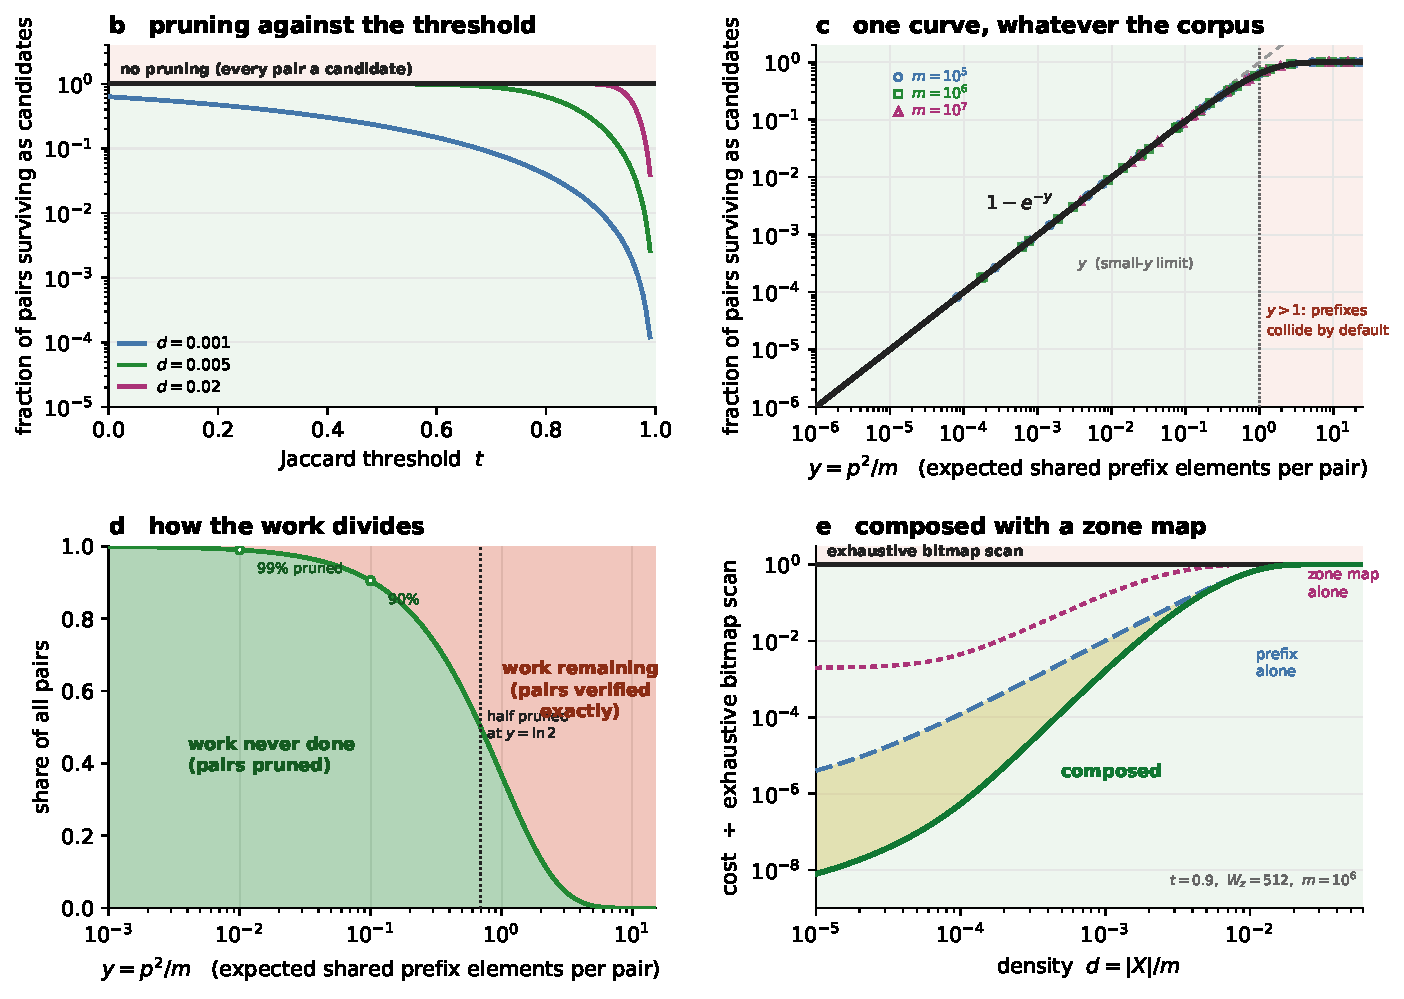
\includegraphics[width=.94\linewidth]{figures/fig3_prefix}
\caption{\textbf{Prefix filtering, analysed on the same terms --- and reducible to a single
variable.} Prefix filtering serves the opt-in thresholded mode, in which only pairs of Jaccard
similarity at least $t$ are reported. With elements in a global order and prefix length
$p(X) = |X| - \lceil t|X| \rceil + 1$, any qualifying pair must share an element between its
prefixes, so indexing prefixes alone answers the thresholded question exactly. Unlike the mechanisms
of Fig.~\ref{fig:pairing-matrix}c--d it is candidate \emph{generation}: the quadratic pair set is
never enumerated.
\textbf{a}, How the rule works. Elements are laid out in a global order --- by document frequency,
rarest first, hence the non-monotonic labels --- and each set's prefix (saturated, bold) is its
rarest $p(X)$ elements, a length that depends on $t$; the remainder is greyed. Any pair with
$J(A,B)\ge t$ must share at least one element between its prefixes. Top: the prefixes have no
element in common, so the pair is discarded without computing any intersection. Bottom: one element
(green) appears in both, so the pair becomes a candidate and is verified exactly.
\textbf{b}, Fraction of pairs surviving as candidates against the threshold, at universe $10^{6}$.
Pruning is governed by how long the prefixes are, and prefix length falls as $t$ rises, so the same
filter that removes almost everything at a high threshold removes almost nothing at a low one --- and
denser operands need a higher threshold to reach the same pruning.
\textbf{c}, All of that collapses onto one curve. For prefixes of length $p$ over a universe of $m$
the expected number of shared prefix elements per pair is $y = p^{2}/m$, and the surviving fraction
is exactly $1 - e^{-y}$ for scattered operands; markers are $(d,t,m)$ combinations drawn at random
across three universe sizes, and they lie on the curve by construction rather than by fit. Two
regimes follow. For $y \ll 1$ the surviving fraction is $y$ itself, so pruning improves
\emph{quadratically} as prefixes shorten. For $y > 1$ prefixes collide by default, essentially every
pair is a candidate, and the index is pure overhead --- the same shape of liability as a summary too
sparse to pay for itself (Fig.~\ref{fig:density-sweep}). The useful operating region is therefore
$y \ll 1$, and $y$ --- not $t$, and not density --- is the quantity a selector should test.
\textbf{d}, The same information as a division of labour: on a linear axis, the share of all pairs
never examined against the share surviving to exact verification. The two are equal at $y = \ln 2$.
\textbf{e}, Prefix filtering composed with a zone map. Unlike the two mechanisms of
Fig.~\ref{fig:density-sweep}c, these \emph{do} compose --- their savings multiply, and the composed
curve tracks the product of the two to within \nm{a factor of 1.25 at the sparsest end, exactly
elsewhere; analytic}. The reason is that they act on different waste \emph{and} read different
statistics of the operands: prefix filtering decides \emph{which} pairs are examined at all, from
element identity, while a zone map reduces the work \emph{within} a pair, from bin occupancy. Both
conditions are needed. Where two mechanisms attack the same waste --- as a zone map and a
representation both do inside one pair --- filtering concentrates what it passes on and the
composition is worth far less than the product; and where two mechanisms read the same statistic,
the second inherits a biased sample from the first even when their granularities differ. At $d = 10^{-3}$, $t = 0.9$ and $W_z = 512$ the composition costs
\nm{$\approx 0.17\%$, analytic} of an exhaustive bitmap scan, against $1.0\%$ for prefix filtering
alone and $16\%$ for a zone map alone.
Analytic throughout; this figure contains no measured data, and like Fig.~\ref{fig:density-sweep} it
models work rather than time. \spec{Real corpora deviate from it in the same direction as elsewhere:
frequency-ordered prefixes concentrate rare elements, so real prefixes collide less than scattered
ones of the same length and the true curve lies below this one.}}
\label{fig:prefix}
\end{figure}

\subsection*{Where the method does not pay}
\label{sec:r6}

Although the best cell beat tuned CRoaring on \prov{17 of 17} corpora tested
above (oracle selection; Table~\ref{tab:corpora}), it does not win
everywhere, and the domain it wins on is worth stating precisely rather than
implying it is universal. The first boundary is the one already drawn by the
density sweep earlier in Results: between the two crossovers sits a band
where nothing beats $\cell{\rB}{\rB}$, and the corpus set above confirms real
data lands there too -- \prov{10 of 17} real corpora are won by
$\cell{\rB}{\rB}$ itself. Reporting that band as a shortfall would misstate the
finding: inside it, the method's job is to recognize the band cheaply and
step aside, not to outperform a kernel that is already optimal there. The
second boundary is that layout, not only content, determines which regime a
dataset falls into. The same genomic cohort sits deep in the sparse regime in
variant-major orientation -- \prov{121--222$\times$} against an all-bitmap
baseline (\texttt{usher\_sarscov2}, \texttt{gnomad\_chr21\_exomes\_af1e-3};
no CRoaring comparison exists for these two) -- but in
haplotype-major orientation lands inside the mid-band, where all-bitmap wins
outright, \prov{0.93$\times$} (\texttt{1KGP3 chr20}, hap.-major; Limitation
L2). This paper does not choose
the orientation a downstream dataset arrives in, and real data gives a large
universe or sparsity far more often than both together.

The third boundary is the selector's own maturity: as established above,
nothing measured in this campaign closes the residual gap to the bucket
oracle. Selection here is cheap, not optimal. None of these three
boundaries undermines the result reported above; together they define its
domain -- representation selection wins broadly, on a stated and bounded
range of corpus shapes, with a known and disclosed edge.

\subsection*{Supplementary tables}
\label{sec:supp-tables}

Storage is a reported trade-off, not an objective this paper optimizes for
(Discussion), so the following three tables are supplementary rather than
main-text, per the display-item allocation (\texttt{NARRATIVE.md} \S7). No
dedicated supplementary file exists yet in this draft; they are placed here,
clearly labelled, until one is built.

% longtable is NOT a float and creates no group, so a bare \scriptsize here
% leaks into every following section. Keep it inside an explicit group.
\begingroup
\scriptsize
\setlength{\tabcolsep}{2.2pt}
\begin{longtable}{@{}p{2.9cm} l r r r r p{4.3cm}@{}}
\caption{\textbf{Supplementary Table S1 | Corpora, provenance and statistics.}
Every corpus referenced anywhere in this paper, in the four provenance groups
used to assemble the benchmark set: \textbf{G1}, the twelve
\texttt{real-roaring-datasets} files CRoaring's own harness runs by default
\cite{chambi2016roaring,lemire2018roaring}; \textbf{G2}, five SNAP social/web
graphs (Stanford Large Network Dataset Collection) scored by
neighbourhood-intersection density; \textbf{G3}, two genomic corpora \emph{present for
scoping, not for the headline} -- included specifically so a reader can judge
whether the benchmark set was chosen favourably, per the standing reviewer
question this table exists to pre-empt; \textbf{G4}, KONECT graphs, UShER
SARS-CoV-2, gnomAD and the \texttt{msprime} coalescent-simulation series,
added after the original survey. Density and mean $|X_i|$ are corpus
properties from the data loaders, not timing results, and are consequently
far more stable than any ratio in Tables~\ref{tab:corpora}--\ref{tab:census}
-- but they still originate in the retired campaign and are marked
provisional like every other number in this draft. For the two G3 corpora,
\emph{universe} and \emph{rows} swap roles between layouts: \texttt{chr20.bin}
is variant-major (universe = 5{,}008 haplotypes, one row per variant site);
\texttt{chr20\_hap.bin} is haplotype-major (universe $\approx$ 1{,}048{,}576
sites, one row per haplotype) -- the layout dependence that Limitation L2 is
about. ---, not reported by the source.}
\label{tab:corpus-inventory}\\
\toprule
Corpus & Group & Rows/sets & Universe $m$ & Mean $|X_i|$ & Density & Origin / notes \\
\midrule
\endfirsthead
\multicolumn{7}{l}{\textit{Supplementary Table S1 (continued)}} \\
\toprule
Corpus & Group & Rows/sets & Universe $m$ & Mean $|X_i|$ & Density & Origin / notes \\
\midrule
\endhead
\midrule \multicolumn{7}{r}{\textit{continued on next page}} \\
\endfoot
\bottomrule
\endlastfoot
\texttt{\seqsplit{census1881}} & G1 & \prov{200} & \prov{4{,}277{,}806} & \prov{5{,}019} & \prov{1.2e-3} & 1881 Canadian census, categorical attributes \\
\texttt{\seqsplit{census1881\_srt}} & G1 & \prov{200} & \prov{4{,}277{,}735} & \prov{3{,}404} & \prov{8.0e-4} & as above, rows sorted \\
\texttt{\seqsplit{census-income}} & G1 & \prov{200} & \prov{199{,}523} & \prov{34{,}610} & \prov{1.7e-1} & US census income (UCI ``Adult''-family), attributes \\
\texttt{\seqsplit{census-income\_srt}} & G1 & \prov{200} & \prov{199{,}523} & \prov{30{,}464} & \prov{1.5e-1} & as above, rows sorted \\
\texttt{\seqsplit{weather\_sept\_85}} & G1 & \prov{200} & \prov{1{,}015{,}367} & \prov{64{,}353} & \prov{6.3e-2} & September 1985 weather observations, binned attributes \\
\texttt{\seqsplit{weather\_sept\_85\_srt}} & G1 & \prov{200} & \prov{1{,}015{,}367} & \prov{80{,}540} & \prov{7.9e-2} & as above, rows sorted \\
\texttt{\seqsplit{wikileaks-noquotes}} & G1 & \prov{200} & \prov{1{,}353{,}179} & \prov{1{,}377} & \prov{1.0e-3} & WikiLeaks cable corpus, term/attribute postings \\
\texttt{\seqsplit{wikileaks-noquotes\_srt}} & G1 & \prov{200} & \prov{1{,}353{,}133} & \prov{1{,}440} & \prov{1.1e-3} & as above, rows sorted \\
\texttt{\seqsplit{uscensus2000}} & G1 & \prov{200} & \prov{36{,}974{,}578} & \prov{30} & \prov{8.1e-7} & US Census 2000; \textbf{sparsest and largest-universe G1 corpus} \\
\texttt{\seqsplit{dimension\_003}} & G1 & \prov{15{,}482} & \prov{3{,}866{,}847} & \prov{91} & \prov{2.4e-5} & Druid-derived dimension column \\
\texttt{\seqsplit{dimension\_008}} & G1 & \prov{5{,}240} & \prov{3{,}866{,}845} & \prov{347} & \prov{9.0e-5} & Druid-derived dimension column \\
\texttt{\seqsplit{dimension\_033}} & G1 & \prov{173} & \prov{3{,}866{,}847} & \prov{22{,}352} & \prov{5.8e-3} & Druid-derived dimension column \\
\addlinespace
\texttt{\seqsplit{as-skitter}} & G2 & \prov{1{,}696{,}415} & \prov{1{,}696{,}415} & \nm{n} & \prov{9.1e-6} & CAIDA skitter internet AS topology, 2005; undirected, symmetrized \\
\texttt{\seqsplit{wiki-Talk}} & G2 & \prov{2{,}394{,}385} & \prov{2{,}394{,}385} & \nm{n} & \prov{2.2e-5} & Wikipedia talk-page edits; directed; only 67{,}492 vertices have out-degree $\geq 2$ \\
\texttt{\seqsplit{soc-Pokec}} & G2 & \prov{1{,}632{,}803} & \prov{1{,}632{,}804} & \nm{n} & \prov{1.6e-5} & Pokec social network (Slovakia); directed; \textbf{lowest skew of the graphs} -- top 1\% of sets hold only 8.8\% of elements \\
\texttt{\seqsplit{com-LiveJournal}} & G2 & \prov{3{,}997{,}962} & \prov{4{,}036{,}538} & \nm{n} & \prov{5.1e-6} & LiveJournal friendship, ground-truth communities; undirected, symmetrized \\
\texttt{\seqsplit{com-Orkut}} & G2 & \prov{3{,}072{,}441} & \prov{3{,}072{,}627} & \nm{n} & \prov{2.7e-5} & Orkut social network; undirected, symmetrized; \textbf{largest input in this set} \\
\addlinespace
\texttt{\seqsplit{chr20.bin}} & G3 (scoping) & \nm{n} & \prov{5{,}008} & \nm{n} & \prov{3.5e-2} & 1/i site-frequency spectrum, 43.6\% singletons; variant-major, universe 626 bytes, L1-resident \\
\texttt{\seqsplit{chr20\_hap.bin}} & G3 (scoping) & \nm{n} & \prov{$\approx$1{,}048{,}576} & \nm{n} & \prov{3.1e-2} & haplotype-major; large universe but 3.1\% dense -- \textbf{nothing beats all-bitmap (0.93$\times$), Limitation L2} \\
\addlinespace
\texttt{\seqsplit{dbpedia-link}} & G4 & \prov{4{,}384{,}102} & \prov{18{,}268{,}993} & \prov{29.8} & \prov{1.63e-6} & KONECT \\
\texttt{\seqsplit{wikipedia\_link\_en}} & G4 & \prov{5{,}978{,}043} & \prov{11{,}206{,}012} & \prov{46.4} & \prov{4.15e-6} & KONECT \\
\texttt{\seqsplit{livejournal-groupmemberships}} & G4 & \prov{2{,}197{,}915} & \prov{7{,}489{,}074} & \prov{48.7} & \prov{6.50e-6} & KONECT, bipartite; universe \textbf{inflated} $\sim$2.3$\times$ (single id space for both columns; true member domain is 3{,}201{,}203) \\
\texttt{\seqsplit{usher\_sarscov2}} & G4 & \prov{29{,}411} & \prov{8{,}451{,}771} & \prov{15{,}769.3} & \prov{1.87e-3} & UCSC UShER SARS-CoV-2; mean dominated by near-universal variants (max 99.7\% carriers), \textbf{median only 404} \\
\texttt{\seqsplit{enwiki-categorylinks}} & G4 & \prov{2{,}165{,}205} & \prov{129{,}698{,}523} & \prov{102.3} & \prov{7.89e-7} & Wikimedia dumps; \textbf{largest universe, lowest density in the full set} \\
\texttt{\seqsplit{gnomad\_chr21\_exomes\_af1e-3}} & G4 & \prov{625{,}656} & \prov{1{,}461{,}894} & \prov{28.2} & \prov{1.93e-5} & gnomAD v4.1 \\
\texttt{\seqsplit{msprime\_10k}} & G4 (sim) & \prov{$\approx$42k} & \prov{2e4} & \prov{1{,}887} & \prov{9.4e-2} & \texttt{\seqsplit{tools/msprime2bin.py}} coalescent simulation; out of target regime \\
\texttt{\seqsplit{msprime\_100k}} & G4 (sim) & \prov{$\approx$51k} & \prov{2e5} & \prov{15{,}720} & \prov{7.9e-2} & as above; out of target regime \\
\texttt{\seqsplit{msprime\_1M}} & G4 (sim) & \prov{$\approx$15.6k} & \prov{2e6} & \prov{136{,}288} & \prov{6.8e-2} & as above; out of target regime \\
\end{longtable}
\endgroup

\begin{table}[!t]
\footnotesize
\setlength{\tabcolsep}{5pt}
\renewcommand\arraystretch{1.05}
\centering
\caption{\textbf{Supplementary Table S2 | Storage cost, bits per value, data
and metadata separated.} Reported the way the Roaring papers report it
\cite{lemire2016roaring}, so corpora of different cardinality are
comparable. \textbf{Metadata is excluded from every column here}: the zone
map and rank index are what the selector needs to \emph{choose} a
representation, not a representation themselves, and folding them into a
data column would hide the cost of the mechanism this paper adds (see
Supplementary Table~\ref{tab:metadata}). \textbf{Best} is the minimum of the
four representation columns, per corpus. On dense corpora the numbers are
Roaring-comparable ($3$--$7$ bits/value); on sparse corpora a dense bitmap
costs $10^{3}$--$10^{6}$ bits/value, which is the storage statement of the
same fact the timing tables make: a bitmap over a large sparse universe is
not a compression scheme, it is a liability (claim A10). All values
\prov{provisional, retired campaign}.}
\label{tab:storage}
\begin{tabular}{@{}l r r r r r r@{}}
\toprule
Corpus & Universe $m$ & Bitmap & Array & Runs & EWAH & \textbf{Best} \\
\midrule
\texttt{census-income} & \prov{199{,}523} & \prov{5.77} & \prov{32.00} & \prov{20.73} & \prov{3.86} & \textbf{\prov{3.08}} \\
\texttt{msprime\_100k} & \prov{200{,}000} & \prov{12.57} & \prov{32.00} & \prov{31.88} & \prov{5.29} & \textbf{\prov{4.44}} \\
\texttt{weather\_sept\_85} & \prov{1{,}015{,}367} & \prov{15.78} & \prov{32.00} & \prov{30.06} & \prov{7.87} & \textbf{\prov{6.77}} \\
\texttt{usher\_sarscov2} & \prov{8{,}451{,}771} & \prov{1{,}080.60} & \prov{32.00} & \prov{2.04} & \prov{4.06} & \textbf{\prov{2.02}} \\
\texttt{wikileaks-noquotes} & \prov{1{,}353{,}179} & \prov{982.89} & \prov{32.00} & \prov{11.36} & \prov{19.46} & \textbf{\prov{10.64}} \\
\texttt{census1881} & \prov{4{,}277{,}806} & \prov{852.27} & \prov{32.00} & \prov{58.86} & \prov{43.79} & \textbf{\prov{29.92}} \\
\texttt{as-skitter} & \prov{1{,}696{,}415} & \prov{1.26e5} & \prov{32.00} & \prov{47.13} & \prov{77.72} & \textbf{\prov{29.26}} \\
\texttt{wikipedia\_link\_en} & \prov{11{,}206{,}012} & \prov{2.68e5} & \prov{32.00} & \prov{46.21} & \prov{72.90} & \textbf{\prov{28.27}} \\
\texttt{dbpedia-link} & \prov{18{,}268{,}993} & \prov{6.38e5} & \prov{32.00} & \prov{56.38} & \prov{101.63} & \textbf{\prov{31.84}} \\
\texttt{uscensus2000} & \prov{36{,}974{,}578} & \prov{1.24e6} & \prov{32.00} & \prov{57.78} & \prov{91.89} & \textbf{\prov{31.98}} \\
\texttt{enwiki-categorylinks} & \prov{129{,}698{,}523} & \prov{3.33e6} & \prov{32.00} & \prov{62.72} & \prov{113.23} & \textbf{\prov{31.85}} \\
\bottomrule
\end{tabular}
\end{table}

\begin{table}[!t]
\footnotesize
\setlength{\tabcolsep}{6pt}
\renewcommand\arraystretch{1.05}
\centering
\caption{\textbf{Supplementary Table S3 | Selector metadata is
universe-proportional, and that is a defect (C33).} \texttt{build\_row()}
constructs the rank index and zone map unconditionally, and both scale with
\textbf{universe}, not cardinality. \textbf{Meta B/row} and \textbf{data
B/row} are bytes of selector metadata and bytes of the chosen data
representation, per row; \textbf{ratio} is meta:data. On
\texttt{enwiki-categorylinks} that is \prov{4} MB of selector metadata
attached to \prov{155} bytes of data -- a \prov{26{,}312$\times$} overhead.
The complement representation already carries the right guard, built only
when $2n > \text{universe}$; rank and occupancy have none. This is a known,
unfixed defect (Limitation L3), not a design choice, and it is why
bitmap-bearing measurements above are restricted to small row counts on the
large-universe corpora. All values \prov{provisional, retired campaign}.}
\label{tab:metadata}
\begin{tabular}{@{}l r r r r@{}}
\toprule
Corpus & Universe $m$ & Meta B/row & Data B/row & Ratio \\
\midrule
\texttt{census-income} & \prov{199{,}523} & \prov{6{,}335} & \prov{13{,}344} & \prov{0.5$\times$} \\
\texttt{weather\_sept\_85} & \prov{1{,}015{,}367} & \prov{32{,}031} & \prov{54{,}497} & \prov{0.6$\times$} \\
\texttt{census1881} & \prov{4{,}277{,}806} & \prov{134{,}784} & \prov{18{,}774} & \prov{7.2$\times$} \\
\texttt{as-skitter} & \prov{1{,}696{,}415} & \prov{53{,}479} & \prov{49} & \textbf{\prov{1{,}083$\times$}} \\
\texttt{dbpedia-link} & \prov{18{,}268{,}993} & \prov{575{,}415} & \prov{113} & \textbf{\prov{5{,}051$\times$}} \\
\texttt{enwiki-categorylinks} & \prov{129{,}698{,}523} & \prov{4{,}084{,}799} & \prov{155} & \textbf{\prov{26{,}312$\times$}} \\
\bottomrule
\end{tabular}
\end{table}

\section*{Discussion}

This paper establishes that choosing which representation pairing to evaluate --- cheaply, from
properties measured online rather than modelled in advance --- dominates the return available from
accelerating any single kernel. A strategy built around avoiding work wins essentially every
asymmetric measurement taken, and the resulting selector outperforms a competitively tuned Roaring
baseline on every real corpus tested, with no single pairing winning enough of the corpus set to make
the matrix itself unnecessary. The shape of the contribution mirrors Roaring's own: array containers,
bitset containers, run containers and SIMD intersection were each individually known before Roaring
existed, and what made the format matter in practice was their composition into one adaptively
dispatched system, evaluated as a whole rather than argued for container by container
\cite{chambi2016roaring,lemire2018roaring}. The claim advanced here is structured the same way --- a
selector over a wider pairing matrix, gated on measured rather than modelled properties, is the
contribution, not any cell inside it.

Roaring already performs adaptive, per-chunk representation choice, so the live question is not
whether adaptivity helps but whether one fixed choice --- a constant chunk width, a constant
cardinality threshold, set once at ingest --- can be right across the whole density axis a corpus is
later evaluated at. This paper's own analysis says it cannot: a fixed threshold is tested against a
chunk's own cardinality rather than the corpus's global density, so a corpus can be dense in aggregate
while every individual chunk stays under the threshold (Table~\ref{tab:census}). Repairing that
threshold inside the incumbent shifts the advantage in opposite directions at the two ends of the
density axis, so neither constant is right and no single fixed threshold serves both regimes. The fix
is offered here as a contribution to the incumbent, not a criticism of it --- Roaring's default is a
memory-sizing crossover, and it is exactly correct for the objective it was chosen for, which is not
this one. What matters for the argument is that the work-avoidance layer keeps its advantage against
the repaired baseline, because that advantage never depended on the kernel underneath being slow.
Roaring needs adaptive selection across density for the same reason this paper's own selector does;
that is the same argument, tested a second time, on someone else's code.

The mechanism behind the asymmetric-cell result is structural rather than incidental. Those cells are
already work-proportional to the smaller operand, so a wider vector instruction has little left to
accelerate; a rank lookup that answers an entire run without reading its bits, or a zone map that
proves two rows disjoint from a fraction of their footprint, wins by removing work rather than by
processing it faster (Fig.~\ref{fig:strategy-decay}a). The complement carries equal weight:
$\cell{\rB}{\rB}$ is where work is genuinely irreducible in the generic case, and it is exactly there
that two decades of vectorized popcount work \cite{mula2018popcount} correctly pay off, including in
this paper's own dense-cell kernel. Avoiding work and accelerating it are complementary axes, not
competing ones, each correct on its own side of the boundary the density sweep locates. That boundary
also responds to the memory hierarchy in opposite directions: vector throughput is a per-cycle
constant a wider core keeps buying more of, realized fully only while data is fed at that rate,
whereas work avoidance removes a count of memory-hierarchy crossings that widening a core does not by
itself reduce (Fig.~\ref{fig:strategy-decay}b). \spec{If core width and the ratio of cache capacity to
DRAM bandwidth continue to diverge as recent processor generations suggest, the boundary measured
here should move further toward avoidance rather than stay where it is} --- a prediction about future
hardware, not a claim about the hardware tested in this study.

The property doing the work throughout this paper is heterogeneity, not sparsity. A corpus in which
every row sits at the same density has nothing for a pairing matrix to exploit, however sparse or
dense that shared density is; what representation selection is paid for is variance in density across
rows that share one universe and one cost model, of which sparsity is only the more familiar half ---
the dense tail rewards exactly the same reasoning, mirrored around the complement. \spec{Read this
way, the same argument should transfer to any workload that mixes elements of very different density
under a shared representation and a shared cost model: sparse linear-algebra format selection among
dense, compressed-sparse-row and coordinate tiles, or a columnar query engine deciding which blocks a
predicate can skip without scanning, are settings where the condition plausibly holds.} Neither has
been tested here, and the claim is offered as where the mechanism should generalize, not as a result
obtained in either domain.

Several things remain open, stated plainly. The selector is cheap relative to the saving it protects,
but it is not close to optimal: nothing measured here closes the residual gap to a bucket oracle that
already knows the winning cell (Fig.~\ref{fig:selection-cost}b). Every measurement reported here is
single-threaded; the real-corpus comparison ran on \nm{one microarchitecture} while the synthetic
cross-architecture comparison spans \nm{four}; and the tile pipeline has so far been evaluated on
within-tile pairs only, with the cross-tile case and the transpose-build cost left to the end-to-end
evaluation that follows this paper. Most directly, the pairing matrix, the selection gate and the tile
pipeline described here are not currently reachable through the project's public C ABI: this paper
reports a systematic measurement of the underlying mechanism, not a released tool, and the ABI and
packaging work needed to close that gap is sequenced immediately after it, with a genome-wide
linkage-disequilibrium application, Tomahawk \cite{tomahawk_github}, as the eventual, and strictly
later, use of the mechanism rather than its motivation. What should outlast any single ratio in this
paper is the map itself --- which representation pairing wins where, and why --- because that map is
transferable independent of the number attached to any one cell.

\section*{Methods}

\subsection*{What makes work avoidable}

This subsection is an existence argument depending on no measurement: a gap must exist between what
a dense-bitmap kernel \emph{spends} and what a cheaper but equally exact algorithm on the same
operands \emph{already achieves}, and representations whose cost is a function of structure rather
than of the universe can enter it. Both compared quantities are achieved; neither lower-bounds the
work the problem demands, and no such bound is claimed here. Every representation is exact and
interconvertible --- \rB, \rS, \rR, \rW\ and the complement view \rC\ encode the same set and every
cell returns the same cardinality --- so nothing is approximated and only the cost changes. Every
quantity in this subsection is a count of stored items or of operations, never a time; constants that convert
these counts to time are empirical and do not enter the derived results. Each result is stated here with its hypotheses; the proof, the worked
numerical checks and the secondary propositions that support but do not themselves state a result are
in Supplementary Note~\ref{note:proofs-avoidance}, for the results up to and including the size bound, and Supplementary Note~\ref{note:proofs-choice}, for the representation-choice optimisation problem that follows it.

Write $A,B \subseteq [0,m)$, $a=|A|$, $b=|B|$, densities $d_A=a/m$, $d_B=b/m$, word width $w$, vector
width $V$ words per operation. Complementation is an involution on density, $d\mapsto 1-d$, so define
the \emph{effective sparsity} $s_X=\min(d_X,1-d_X)\in[0,\tfrac12]$ and $s=\min(s_A,s_B)$.

\paragraph*{What cardinality alone determines.}
Given only $a$ and $b$ --- the cheapest metadata any selector holds --- the answer is confined to
\begin{equation}
\max(0,\,a+b-m) \;\le\; |A \cap B| \;\le\; \min(a,\,b),
\label{eq:interval}
\end{equation}
and every integer in the range is realised (Supplementary Note~\ref{note:proofs-avoidance}). Its width is the quantity the rest
of this subsection turns on:
\begin{equation}
\min(a,b)-\max(0,a+b-m) \;=\; \min\,(\,a,\;b,\;m-a,\;m-b\,) \;=\; m\,\min(s_A,s_B) \;=\; m\,s .
\label{eq:width}
\end{equation}
The four terms are the sizes of the four lists one could enumerate --- $A$, $B$, $A^{c}$, $B^{c}$ ---
so the uncertainty is the size of the smallest, and one near-empty or near-full side collapses it
alone. Above density one half the floor lifts off zero at $(d_A+d_B-1)m$: at $d_A=d_B=0.51$, two per
cent of the universe must overlap.

\paragraph*{The fixed cost, and therefore the headroom.}
A dense bitmap stores $\lceil m/w\rceil$ words whatever it contains, so $\cell{\rB}{\rB}$ performs
$\lceil m/(wV)\rceil$ vector AND-plus-popcount operations per pair, independently of $a$, $b$, of
structure, and of the answer. Against that, suppose each operand $X$ is available as a bitmap and as a
sorted array of whichever of $X$, $X^{c}$ is smaller --- $\Theta(m\,s_X)$ of space, the choice made
from $a$, $b$, $m$ in $O(1)$; no rank index is needed for this result. Then $|A\cap B|$ is answered in
$O(m\,s)$ membership probes (four cases, one per term of Eq.~\eqref{eq:width}; Supplementary Note~\ref{note:proofs-avoidance}).
Counting descriptor items touched, and taking $w \mid m$,
\begin{equation}
\frac{\text{items touched by } \cell{\rB}{\rB}}{\text{items touched by the cheapest list-based cell}}
\;=\; \frac{\lceil m/w\rceil}{m\,s} \;=\; \frac{1}{w\,s},
\label{eq:headroom}
\end{equation}
which exceeds one whenever $s<1/w$ and grows without bound as either operand leaves density one half
--- the headroom, derived rather than observed, and a comparison of two \emph{achieved} costs, not a
lower bound on any algorithm's work. Two of the four cases need a complement view, which is why \rC\
is part of the design rather than an afterthought for the dense tail. Charging measured per-item
costs --- a random probe against a vector word --- turns it into a crossover in $s$ of
\nm{measured crossover in effective sparsity}.

\paragraph*{From descriptor length to operation count.}
Everything else here counts \emph{stored items}, a fact about representation size; the paper's claim
is about work. One identity carries that step. Let $A$ be a bitmap with an $O(1)$ rank index,
$\mathrm{rank}_A(i)=|A\cap[0,i)|$, and $B$ a run container with maximal runs
$\{[u_i,v_i)\}_{i=1}^{r}$. The runs partition $B$, so
\begin{equation}
|A \cap B| \;=\; \sum_{i=1}^{r}\big(\,\mathrm{rank}_A(v_i)-\mathrm{rank}_A(u_i)\,\big),
\label{eq:rank}
\end{equation}
in exactly $2r$ lookups --- independent of $m$, of $|A|$, of $|B|$, and of the run lengths
(Supplementary Note~\ref{note:proofs-avoidance}). A run of any length is priced as a run of length one, because the kernel never
looks inside it; symmetrically $\cell{\rR}{\rR}$ by merge costs $O(r_A+r_B)$ with no index. This is
what makes a run count a cost parameter and not merely a storage parameter, and it is the only bridge
between the two here: it reaches \emph{operation count}, not time, since per-operation constants still
differ across cells.

\paragraph*{What randomness would predict.}
Let each position be set independently with probability $d$, and write $\kappa(\rho)$ for the number
of stored items representation $\rho$ must touch. The bitmap and array entries are exact; the run and
fill-compressed entries are the leading-order forms of exact Bernoulli expectations (Supplementary Note~\ref{note:proofs-avoidance}), written in
$s=\min(d,1-d)$,
\begin{equation}
\mathbb{E}\,\kappa(\rB) = \Big\lceil \tfrac{m}{w} \Big\rceil, \quad
\mathbb{E}\,\kappa(\rS) = m\,d, \quad
\mathbb{E}\,\kappa(\rR) = m\,d(1-d) = m\,s(1-s), \quad
\mathbb{E}\,\kappa(\rW) = \tfrac{m}{w}\big[\,1-(1-s)^{2w}-s^{2w}\,\big],
\label{eq:expected}
\end{equation}
where $\kappa(\rR)$ counts maximal runs and $\kappa(\rW)$ literal words plus fill groups. None of
these expectations is new. The \rW\ row is the word-aligned expected-size model of Wu, Otoo and
Shoshani \cite{wu2006wah}, whose bracket is identical to the one above under their payload width of
$w-1$ bits per word rather than $w$; the symmetry about $d=\tfrac12$ and the resulting
incompressibility at that density are theirs as well. The \rR\ row is the classical expected run
count for a uniformly random arrangement \cite{mood1940runs}, and the interval bound is
the Fr\'echet--Boole inequality. The density--clustering parameterisation is also due to
\cite{wu2006wah}; the design space it spans has since been mapped empirically for Roaring, WAH and
tree-encoded bitmaps by Lang et al. \cite{lang2020teb}, who report that an uncompressed bitmap reads
faster than any of the three compressed formats over $16 \le f \le 128$ and $0.01 \le d < 1$, and
that they expect ``a performance-optimized implementation to dominate an even larger space'' than
their unoptimized baseline did. That is the headroom this paper measures, stated from the compressed
side. They are restated here in one notation because the pairing matrix needs them as
inputs, not because they are results of this paper. With the
complement view making the best of \rS\ and $\rC\!\circ\!\rS$ cost $m\,s$, every entry is constant in
$s$ or strictly increasing on $[0,\tfrac12]$ and symmetric about $d=\tfrac12$: under this null model the
U-shaped cost curve is a theorem --- about the model and the bitmap's flatness, not about any method.
Randomness gives run containers nothing either, since
$\tfrac12 m s\le\mathbb{E}\,\kappa(\rR)\le m\,s+1$, so choosing \emph{among} \{\rS,
$\rC\!\circ\!\rS$, \rR, \rW\} buys at most a constant on structureless data. \rB\ is the exception and
the exception is the point: $\kappa(\rB)$ is $\lceil m/w\rceil$ at every density, so the spread across
the full matrix is Eq.~\eqref{eq:headroom} and unbounded. It is the envelope, not each cell, that
follows $\Theta(\min(m/w,\,m\,s))$.

\paragraph*{The deviation, which is the contribution.}
Real data is not random, and the representations part company with Eq.~\eqref{eq:expected} in a way
density cannot express. At fixed density $d\le\tfrac12$ with $k=dm$, $\kappa(\rB)$ and $\kappa(\rS)$
are constants, while $\kappa(\rR)$ ranges over every integer in $[1,k]$ and $\kappa(\rW)$ from $O(1)$
to $\Theta(\min(k,m/w))$ (proved by explicit families in Supplementary Note~\ref{note:proofs-avoidance}). Writing
$\sigma(\rho,X)$ for predicted descriptor length at $X$'s density over actual, $\sigma$ is identically
one for \rB\ and \rS, at least $\max(d,\,1-d+\tfrac{1}{m})\ge\tfrac12$ for \rR, and unbounded above:
real rows can be arbitrarily cheaper than random rows of the same density and at most about twice as
expensive.

One impossibility follows, exactly. A selector reading density --- or cardinality, or any function of
them --- evaluates one fixed function on every row of that density, so by the range above it
mis-predicts $\kappa(\rR)$ by an unbounded factor on some rows at every density; a fixed representation
cannot exploit $\sigma$ either, having committed before $\sigma$ is knowable. That rules out a family
of selectors without choosing among the survivors, and two further readings do not follow: whether a
mis-predicting model costs more than selecting nothing depends on which cell it picks and that cell's
actual cost, which is measured (Fig.~\ref{fig:selection-cost}b), not derived; and a run or occupancy
count is $O(1)$ metadata that sees $\sigma$ perfectly and could feed a model. What is proved is that
selection must be gated on a statistic that sees structure rather than on cardinality --- structural
summary or direct kernel measurement is resolved by the measured selector comparison in
Fig.~\ref{fig:selection-cost}b.

\paragraph*{The null model is a floor, and it is the same floor three times.}
Independent placement at fixed density is the \emph{extremal} arrangement for every mechanism used
here, always in the same direction (proofs in Supplementary Note~\ref{note:proofs-avoidance}). For a representation,
Eq.~\eqref{eq:expected} sits within a factor of two of the worst achievable descriptor. For a zone map
of bin width $W_z$, scattering maximises the occupied-bin fraction, so the summary's null cost is an
upper bound on its cost and a lower bound on its value. For the prefix filter of the narrowed-contract
mode, the entire mechanism depends on the operands through one dimensionless quantity, and any ordering
that concentrates rare elements into prefixes makes real prefixes collide less often than scattered
ones of the same length. In each case the null is what the mechanism is worth on data with no
structure to find, real data deviates from it only in the mechanism's favour, and that deviation is
exactly the quantity the mechanism converts into avoided work.

\paragraph*{The mid-density regime selects bitmap throughput.}
At $s=\tfrac12$ the interval has width $m/2$ and excludes nothing, the cheapest list-based cell spends
$m/2$ probes against $\lceil m/w\rceil$ words, and Eq.~\eqref{eq:expected} offers neither \rR\ nor \rW\
an advantage: Eq.~\eqref{eq:headroom} falls below one. In the generic case the mid-density band belongs
to $\cell{\rB}{\rB}$, and a selector choosing it there is correct rather than defeated. This bounds what
cardinality determines absent structure, not what any kernel must spend --- call it a \emph{metadata}
or \emph{identifiability floor}, never an information-theoretic one --- and a structured row at exactly
this density is a counterexample to the unqualified form (Supplementary Note~\ref{note:proofs-avoidance}).
Zone-map occupancy remains informative in this band because it records arrangement that cardinality
does not.

\paragraph*{Why the two mechanisms are selected between rather than stacked.}
Composing a zone map with a representation is not the product of the two, because filtering
\emph{concentrates} what it passes on: conditioned on a bin of width $W_z$ being occupied its expected
local density is $d/p$, $p=1-(1-d)^{W_z}$, not $d$ --- no summary hands a kernel anything sparser than
one bit per bin (Supplementary Note~\ref{note:proofs-avoidance}). Charging the summary pass $c/W_z$ of a bitmap scan and taking
the operands independent, the composed cost relative to a plain bitmap is
\begin{equation}
\frac{c}{W_z} \;+\; p_A\,p_B\;\kappa\!\Big(\frac{d}{p}\Big),
\label{eq:compose}
\end{equation}
$\kappa\le1$ being the envelope of Eq.~\eqref{eq:expected} normalised against the bitmap. The
composition never costs more than the summary alone, yet is floored at $c/W_z$, below which a sparse
representation is cheaper outright --- three regimes, the middle one exactly $x e^{-x} > c/w$ in
$x = W_z d$ bits per bin, opening where the summary undercuts enumeration and closing where bins stop
being empty. This is the analytic form of the gating result of Fig.~\ref{fig:selection-cost}c, and it
models \emph{work}: it bounds where a filter has work to remove and says nothing about what one costs
when it removes nothing.

\paragraph*{Each mechanism's liability is two-sided, for unrelated reasons at the two ends.}
A summary is indexed by the universe while every compressed representation is indexed by the data, so
their costs must cross. Charging the summary $c/W_z$ of a bitmap scan as in Eq.~\eqref{eq:compose},
and a one-word-per-element representation $w\,d$, the low crossing is
\begin{equation}
d_{\mathrm{low}} \;=\; \frac{c}{w\,W_z} \;=\; 3.1\times10^{-5} \qquad (c=1,\; w=64,\; W_z=512),
\label{eq:dlow}
\end{equation}
below which reading the summary costs more than enumerating the operands outright (Supplementary Note~\ref{note:proofs-avoidance}). At the other end $p_Ap_B\to1$: no bin is empty, the summary proves nothing, and only its own
$c/W_z$ remains. A run- or fill-based representation crosses at its own density, wherever its
descriptor length falls below $m/W_z$, but that a crossing exists at all is generic. Prefix filtering
has the same shape in $y=p^2/m$: for $y\ll1$ the surviving fraction is $y$ itself, so pruning improves
quadratically as prefixes shorten, while for $y>1$ prefixes collide by default and the index earns
nothing. This is why no mechanism here is applied unconditionally, and why each gate is a two-sided
test rather than a threshold.

\paragraph*{A narrowed contract, and what two integers then settle.}
Every statement above returns the cardinality itself. A caller may instead ask a narrower question ---
report only the pairs with $J(A,B)\ge t$, or only those with $|A\cap B|\ge\tau$, or restrict attention
to operands whose size falls in a band --- and the narrowing is itself exploitable, because
Eq.~\eqref{eq:interval} already says what sizes permit:
\begin{equation}
J(A,B) \;=\; \frac{|A\cap B|}{|A\cup B|} \;\le\; \frac{\min(a,b)}{\max(a,b)},
\label{eq:sizebound}
\end{equation}
so $J(A,B)\ge t$ requires $\min(a,b)\ge t\,\max(a,b)$, and $|A\cap B|\ge\tau$ requires
$\min(a,b)\ge\tau$ (proof in Supplementary Note~\ref{note:proofs-avoidance}). The hypotheses are that $a,b>0$ and $t\in(0,1]$;
nothing is assumed about arrangement, about $m$, or about how either operand is stored. Both conditions
are necessary and neither is sufficient, so the test discards pairs and never reports one --- the
survivors still go to an exact kernel, at the cost of one comparison between two integers already held
as metadata, no element of either set read. This is the Swamidass--Baldi pruning bound
\cite{swamidass2007bounds} together with the size (length) filter of
\cite{arasu2006exact}, in the two-sided form standardised by \cite{mann2016empirical} and applied
jointly with prefix filtering to Tanimoto over binary vectors by \cite{anastasiu2016tapnn}, restated here to place it against the mechanisms above
rather than as a result of this paper.
The operational narrowing and complete thresholded construction are given in Supplementary
Note~\ref{note:threshold}.

\paragraph*{What that removes, and why a wider corpus helps it.}
Modelling a corpus by drawing cardinalities independently with $\log a$ uniform on $[0,\ln K]$ --- the
density $\Pr(a)\propto 1/a$, exactly the $1/i$ cardinality spectrum this paper's benchmark protocol
mandates (``Corpora, provenance and loaders''), not an approximation to it ---
$\min(a,b)/\max(a,b)\ge t$ becomes $|\log a - \log b|\le\gamma$, $\gamma=\ln(1/t)$, and for two
independent uniforms on an interval of length $L=\ln K$,
\begin{equation}
\Pr\big[\text{pair can qualify}\big] \;=\; 1-\Big(1-\frac{\ln(1/t)}{\ln K}\Big)^{2},
\qquad \ln(1/t)\le\ln K,
\label{eq:survive}
\end{equation}
with the absolute form $\big(1-\ln\tau/\ln K\big)^{2}$ (proof and worked values in Supplementary Note~\ref{note:proofs-avoidance}, which agree with a $10^{5}$-sample simulation to three decimals). Expanding for small $\gamma$
gives $2\gamma\!\int\!\phi^{2}$ for any density $\phi$ of $\log a$, so the governing quantity is the
\emph{effective log-spread} $1/\!\int\!\phi^{2}$ of the size distribution, of which
Eq.~\eqref{eq:survive} is the log-uniform case. Two hypotheses carry real weight. Cardinalities are
integers, and $a=b$ passes at every $t$, so the continuous form is optimistic where sizes are small.
And the favourable scaling in $K$ --- Eq.~\eqref{eq:survive} decreases monotonically in $K$ --- is a
property of the log-uniform family and not of heavy tails generally: under the alternative reading in
which \emph{ranked} sizes scale as $1/i$, the surviving fraction is exactly $1-t$, independent of $K$,
since the effective log-spread saturates at two nats however far the sizes are spread. The favourable
scaling in $K$ is therefore claimed for the spectrum this paper benchmarks, not for every skewed
corpus.

\paragraph*{The size bound does not multiply with the within-pair mechanisms.}
Acting at a coarser granularity is not sufficient for savings to compose. The size test decides
whether a pair is formed at all, while representation choice and the zone map act inside a pair that
is formed, so the granularity argument of Eq.~\eqref{eq:compose} predicts a product --- and the
product is not achieved, because both mechanisms read the same statistic. The survivors of
Eq.~\eqref{eq:sizebound} are the pairs with $a\approx b$, and every within-pair mechanism is cheapest exactly
when $a$ and $b$ are \emph{dissimilar}, since its cost tracks $\min(a,b)$ against a fixed
$\lceil m/w\rceil$. Conditioning raises the mean cost of a survivor by
\begin{equation}
\frac{\mathbb{E}\big[\min(a,b)\;\big|\;\min/\max\ge t\big]}{\mathbb{E}\,\min(a,b)}
\;=\; \frac{L^{2}\big(K(1-t)-\gamma\big)}{\gamma\,(2L-\gamma)\,(K-L-1)}
\;\xrightarrow[\;t\to1\;]{}\; \frac{\ln K}{2},
\label{eq:shortfall}
\end{equation}
and the composed work exceeds the product of the two savings by that same factor; the derivation, the
numerical verification and the decorrelation control that isolates the shared statistic as the cause
are in Supplementary Note~\ref{note:proofs-avoidance}. The composition is still strongly worth taking. What is
refuted is only the product; the general rule is that mechanisms compose multiplicatively when they act
on different waste \emph{and} are driven by different operand statistics, and sharing a statistic costs
the composition Eq.~\eqref{eq:shortfall}'s factor even across granularities. Values here are analytic,
computed over the model above at $m=10^{6}$, and count work rather than time.

\paragraph*{Choosing a representation is a different problem from choosing a size, and only one of
them is separable.}
Everything above prices representations; a deployed library must \emph{choose} between them, and the
choice has to be stated as an optimisation before it can be called optimal. Partition the universe into
chunks of $M$ bits, each stored in one representation, $n=M/w$ words to a chunk and $e$ bits to a
stored array element. Given a corpus, a distribution $\pi$ over the chunk pairs an application
evaluates, and an operation $\omega$, the problem is to choose an assignment $\rho$ of representations
to chunks minimising $\sum_{(x,y)\sim\pi} C_\omega(\rho(x),\mu_x;\rho(y),\mu_y)$ subject to a byte
budget, where $\mu$ is the metadata of Eq.~\eqref{eq:expected} and $C_\omega$ counts items touched at
measured per-item constants. Storage is a \emph{separable} objective --- minimised one container at a
time --- whereas the query cost is quadratic in the assignment, since there is no such thing as the
cost of a container, only the cost of a pair (Supplementary Note~\ref{note:proofs-choice}). And the incumbent's three
container decisions --- array against bitset, array against run, bitset against run --- are one rule,
$\arg\min$ over serialized size, so its array-to-bitset threshold is $\tau_{\mathrm{stor}} = M/e$, a
property of the format carrying no machine constant and no property of the workload: the exact optimum
of a separable objective, and why it can be a compile-time constant. What follows is what changes
when the objective is not separable.

\paragraph*{The crossover is a formula, and the two constants in the field are its two limits.}
Write $c_w$ for a vectorised word \texttt{AND}-plus-popcount, $c_p$ for a membership probe into a
bitmap and $c_m$ for a merge step, and $\theta_{pw}=c_p/c_w$, $\theta_{mw}=c_m/c_w$. Promotion of a
chunk of cardinality $k$ from array to bitset is favourable against a bitmap partner exactly above
\begin{equation}
\tau_{\cap} \;=\; \frac{c_w}{c_p}\cdot\frac{M}{w}\;=\;\frac{n}{\theta_{pw}},
\qquad\text{whence}\qquad
\frac{\tau_{\mathrm{stor}}}{\tau_{\cap}} \;=\; \frac{w}{e}\,\theta_{pw},
\label{eq:tauratio}
\end{equation}
and against an array partner above $(\theta_{pw}/\theta_{mw}-1)\,k_Y$ for a partner of size $k_Y$
(proof in Supplementary Note~\ref{note:proofs-choice}). Pricing a byte at $\lambda\ge0$ and minimising query cost plus
$\lambda\,\mathrm{bytes}$ gives a threshold that runs from $\tau_{\cap}$ at $\lambda=0$ to
$\tau_{\mathrm{stor}}$ as $\lambda\to\infty$: every value between the two is optimal at some price of a
byte, and $\tau_{\mathrm{stor}}=M/e$ is the unique threshold at which promotion is never paid for in
bytes. The threshold also carries the pair count, so under any byte budget the optimum is not a
function of the container at all. The measured input is the symmetric crossover \nm{cardinality at
which an array--array merge stops beating a bitmap--bitmap popcount}, which fixes $\theta_{mw}$;
substituted into Eq.~\eqref{eq:tauratio} at $M=2^{16}$, $w=64$, $e=16$ together with \nm{measured ratio
of a bitmap probe to a merge step} it gives \nm{the ratio of the two thresholds}, recovering the
divergence between the two objectives from measurements of the constants and no free parameters. Both
crossovers share $c_w$, so measuring them together over-determines the model and the probe-to-merge
ratio becomes a checkable prediction rather than an input.

\paragraph*{A fixed threshold is optimal, under five hypotheses, and each of them fails.}
The loose form is false, so state the hypotheses first: if the candidates are
only \rS\ and \rB, the operation is a count-only intersection, the per-item constants do not depend on
the resident footprint, there is no byte budget, and every chunk faces the same partner mix, then the
optimal assignment \emph{is} the fixed threshold $\tau_{\cap}$ of Eq.~\eqref{eq:tauratio} --- a machine
constant, independent of the corpus. Dropping any one hypothesis breaks it, with an exact witness for
each (Supplementary Note~\ref{note:proofs-choice}): admitting \rR\ reintroduces the impossibility above, specialised to the
container decision, since $\cell{\rR}{\rB}$ costs a strictly increasing function of run count while
$\cell{\rS}{\rB}$ does not depend on it; letting the partner mix vary makes the optimal threshold
\begin{equation}
\tau^{*}(\beta,\bar k)\;=\;\frac{\beta\,c_w n+(1-\beta)(c_p-c_m)\,\bar k}
                                 {\beta\,c_p+(1-\beta)\,c_m},
\label{eq:taustar}
\end{equation}
where $\beta$ is the pair-weighted fraction of a chunk's partners that are bitmaps and $\bar k$ the
mean cardinality of the array partners: a statistic of the workload rather than of the machine, and
self-referential --- an optimal fixed
threshold is a fixed point $\tau=\tau^{*}(\beta(\tau),\bar k(\tau))$, which exists but need not be
unique; admitting a byte budget makes the threshold its dual variable, sweeping the whole interval
above; changing the operation flips the matrix's sign, since cardinality queries have no operation
dimension at all (union, difference and symmetric difference are inclusion--exclusion over the
intersection) but a \emph{materialising} union with a bitmap operand costs $n$ words whatever the other
side is, so no single stored assignment serves a mixed workload. The fifth hypothesis --- that the
per-item constants do not depend on footprint --- is the one that is not analytic and the one the
measurements say dominates: $c_w$ is not a constant, footprint re-enters through it, and a work model
that prices the choice cannot price its consequence, the same divergence recorded under
Eq.~\eqref{eq:compose} and treated as a measurement question, not an analytic one.

\paragraph*{Metadata settles the decision wherever the decision matters.}
Two identifiability questions must not be merged. Eq.~\eqref{eq:width} says what cardinality
determines about the \emph{answer}, pinned only at the density extremes. What cardinality determines
about the \emph{decision} is different and more favourable: every cost in this paragraph and the two
before it is a closed form in $(k,r,\ell+g)$ and the constants, so a selector holding those three
integers per operand evaluates the ordering exactly, in $O(1)$, touching no operand data --- which is
what ``selection must be near-free'' means, and a consequence of the cost model rather than an
engineering aspiration (proof in Supplementary Note~\ref{note:proofs-choice}). Holding only $k$, the ordering is not
determined once \rR\ is a candidate; one extra integer restores it and more cardinality precision does
not. Suppose the constants are known within a factor $\eta\ge1$ --- the uncertainty of the modelled
costs, distinct from the $\gamma$ of the size bound above --- and let $\Lambda$ be the ratio of the two
cheapest modelled costs: if $\Lambda>\eta$ the ordering is determined; if $\Lambda\le\eta$ it is
not, and choosing the second-best costs at most $\eta$. So for every pair, either the metadata
settles the decision or the decision does not matter to within the precision of the constants, and the
undetermined set is an $\eta$-neighbourhood of the boundaries rather than a region of unbounded error.
The caveat that makes $\eta$ interesting: it is the uncertainty of the \emph{model}, and where the
model omits the memory system it is not small --- the derived reason to measure a candidate rather than
only to model it.

\paragraph*{Why an advantage survives repairing the kernel beneath it.}
A pairwise batch costs $C_{\mathrm{meta}}$ plus the cell cost summed over the pairs a summary does not
discard and the regions it does not exclude; those sets are functions of cardinality, bin occupancy and
the data, and of nothing else, so no change of representation moves either set (Supplementary Note~\ref{note:proofs-choice}).
Consequently, if a better kernel divides every cell cost by $\alpha$, the advantage over the same batch
without avoidance is invariant in $\alpha$ when the summary is free and erodes only through the
summary's share of the surviving cost: improving a kernel cannot subsume avoidance, because avoidance
changes which work is asked for and a kernel changes only what asked-for work costs. Which savings
multiply is settled by the same rule as Eq.~\eqref{eq:shortfall}: a zone map reads bin occupancy while
representation choice reads cardinality and run count, so those multiply; the size bound reads
cardinality, which representation choice also reads, so those do not, and a container-threshold gain
must not be multiplied into a size-bound gain. Quantitatively, against an incumbent already holding the
compute-optimal threshold of Eq.~\eqref{eq:tauratio}, the modelled advantage of adding a zone map of bin
width $W_z$ peaks at
\begin{equation}
G_{\max}\;=\;\frac{\theta_{pw}\,w}{2\sqrt{c\,W_z}}
\qquad\text{at}\qquad d^{*}=\frac{\sqrt{c}}{W_z^{3/2}},
\label{eq:gmax}
\end{equation}
valid on $(\theta_{pw}w\sqrt{c})^{2/3}\le W_z\le\theta_{pw}w$ and saturating at
$\sqrt{\theta_{pw}w/c}\,/2$ above it, and falling below one outside a window whose lower edge is
Eq.~\eqref{eq:dlow} with the per-item constants carried, $c/(\theta_{pw}wW_z)$ (proof in Supplementary Note~\ref{note:proofs-choice}). Eq.~\eqref{eq:gmax} is a \emph{null-model} ceiling on structureless data, and by the
one-sidedness of $\sigma$ above, real corpora can only fall below the null, so a measured advantage
exceeding it is evidence of structure and must be reported as such rather than as agreement. And
Eq.~\eqref{eq:gmax} excludes the narrowed contract entirely: Eq.~\eqref{eq:survive} supplies its own
factor, and by the rule above the two are not multiplied.

\paragraph*{The irreducible regime selects throughput.}
The mid-band above is not only where these results stop applying; it is where a different optimization
applies, and the two are complementary rather than competing. Where Eq.~\eqref{eq:headroom} falls below
one and $p_Ap_B\to1$, the work $\cell{\rB}{\rB}$ performs is, in the generic case, work that is going to
be performed, and what remains to optimize is the per-cycle throughput of its $\lceil m/(wV)\rceil$
vector \texttt{AND}-plus-popcount operations --- a quantity none of the results above speaks to, and one
the popcount literature has already driven close to the hardware limit \cite{mula2018popcount}.
Eq.~\eqref{eq:headroom} and Eq.~\eqref{eq:compose} locate the boundary between the two domains; they do
not rank them.


\subsection*{Representations and the per-cell cost model}

Each row --- one set $X_i$ over a shared universe of $m$ bits --- is stored in one of several
representations, each with a distinct asymptotic cost for computing an intersection
\emph{cardinality}, $|X_i \cap X_j|$, rather than the intersection itself. We define each
representation below, together with the cost of the cell it forms when paired with itself or with
another representation; every cost-model symbol used elsewhere in this paper is defined here and only
here.

Four representations form the symmetric pairing matrix. A dense bitmap (\rB) stores $m$ bits directly,
one per universe position, and costs $\Theta(m)$ to intersect against another dense bitmap by AND and
popcount, independent of either side's cardinality. A sorted array (\rS) stores the set's
$|X|$ set positions as sorted integers and costs $\Theta(|X|)$ against a bitmap, since each element is
resolved by a single random probe. A run container (\rR) stores the set as $r$ maximal runs
$(a,b)$ of contiguous set bits and, against a bitmap fitted with a rank index (below), costs
$\Theta(r)$ --- independent of run length. A fill-compressed word stream (\rW, an EWAH-style
encoding of literal words interleaved with run-length-coded fill words) costs
$\Theta(\ell + g)$ against a bitmap, where $\ell$ is the literal-word count and $g$ the fill-group
count, and its fills are skipped in constant time using the same rank index used for \rR. A fifth
view, the complement (\rC), does not add a representation to the symmetric matrix; it is a strategy,
described in the next subsection, for reusing whichever of \rB, \rS, \rR or \rW is cheapest on a
row's complement when that row sits above density one-half.

The cost of each symmetric cell is, in the notation above: $\cell{\rB}{\rB}=\Theta(m)$ (naive; made
sub-linear by the zone-map filter below); $\cell{\rB}{\rS}=\Theta(|S|)$; $\cell{\rB}{\rR}=\Theta(r)$
with a rank index; $\cell{\rB}{\rW}=\Theta(\ell+g)$; $\cell{\rS}{\rS}=\Theta(|A|+|B|)$ by merge or
$\Theta(|A|\log(|B|/|A|))$ by galloping search when $|A|\ll|B|$; $\cell{\rS}{\rR}=\Theta(|S|+r)$ by
merge or $\Theta(|S|\log r)$ by binary search into runs; $\cell{\rS}{\rW}=\Theta(|S|+\ell+g)$;
$\cell{\rR}{\rR}=\Theta(r_A+r_B)$ by run merge; $\cell{\rR}{\rW}=\Theta(r_A+(\ell+g)_B)$; and
$\cell{\rW}{\rW}=\Theta((\ell+g)_A+(\ell+g)_B)$. Every cell except $\cell{\rB}{\rB}$ is sub-linear in
the universe size $m$. The formal statement of what these costs imply --- that the null model is a
floor rather than a prediction, and the exact conditions under which no representation beats a bitmap
--- is given with full proofs in Supplementary Note~\ref{note:proofs-avoidance}.

\subsection*{The pairing matrix and its cells}

The paper reports the ten cells of the
symmetric representation matrix formed from \{\rB, \rS, \rR, \rW\}: \cell{\rB}{\rB}, \cell{\rB}{\rS},
\cell{\rB}{\rR}, \cell{\rB}{\rW}, \cell{\rS}{\rS}, \cell{\rS}{\rR}, \cell{\rS}{\rW}, \cell{\rR}{\rR},
\cell{\rR}{\rW}, \cell{\rW}{\rW}. The complement strategy, \cell{\rC}{\rB}, is an eleventh, asymmetric
strategy rather than a twelfth symmetric cell: when a row's density places it above one-half, its
complement is computed and intersected using whichever of the ten cells above is cheapest for that
complement, and the requested cardinality is recovered by inclusion--exclusion,
$|A \cap B| = |B| - |A^{c} \cap B|$, where $A^{c}$ is $A$'s complement against the shared universe.
This convention is used consistently throughout: any count of ``ten'' cells in this paper refers to
the symmetric matrix over \{\rB, \rS, \rR, \rW\}, and \cell{\rC}{\rB} is reported separately as a
strategy rather than folded into that count. Roaring is never constructed as a cell of this matrix; it
is used throughout as an external baseline only (below).

Each cell is implemented independently against a shared representation layer providing one view per
format (bitmap, sorted list, run, EWAH-fill and complement). Several of the asymmetric cells have more
than one implemented strategy --- for example \cell{\rB}{\rR} has a rank-indexed variant and a scalar
per-run-scan variant --- and each variant was raced against the independent oracle described below
before being admitted to any comparison. The variant reported for a given cell in Results is the one
selected as fastest for the density regime or corpus shape being reported, not a single fixed
implementation chosen in advance; the full record of implemented variants, including those that did
not win any regime, is not itemized in this paper (Code availability).

\subsection*{Zone-map and rank-index construction}

Two mechanisms let a kernel decide how much of a row it needs to visit, rather than visiting all of it
faster. To decide how much of a dense row a pairing needs to scan, we used a \emph{zone map}, a
bitmap of coarser granularity in which bit $k$ records whether bin $k$ of the underlying row --- a
contiguous block of \nm{zone-map bin width in bits} bits --- contains any set bit. To answer a run's
or a fill's contribution to a bitmap without touching the bits it spans, we used a \emph{rank
(prefix-popcount) index}, following the rank/select lineage of Jacobson, Clark and Vigna's
\texttt{rank9} \cite{jacobson1989succinct,clark1996compact,vigna2008broadword}.

The zone map is built by a single forward pass over the row, or is free at query time when the
underlying storage already carries block-occupancy metadata, as columnar formats commonly do; its
storage cost is \nm{zone-map storage cost as a fraction of the bitmap it summarizes} of the bitmap it
summarizes. For a pair, the bitwise AND of the two rows' zone maps, $\mathrm{occ}_A \wedge
\mathrm{occ}_B$, is itself a bitmap of $m/\nm{zone-map bin width in bits}$ bits, and its popcount is
the \emph{exact} number of bins the pairing needs to visit, not an estimate: a popcount of zero proves
the two rows disjoint without visiting either. The rank index is built by a single forward
prefix-popcount pass and stores \nm{rank-index storage cost as a fraction of the bitmap it indexes} of
the bitmap it indexes; for a run or fill spanning positions $[a,b)$ on the indexed side, its
contribution to the intersection is answered in constant time as
$\mathrm{rank}_B(b) - \mathrm{rank}_B(a)$, the number of set bits in $B$ up to $b$ minus the number up
to $a$ --- this formula is used, unchanged, by every cell that pairs a run- or fill-based
representation against an indexed bitmap.

Neither mechanism is applied unconditionally. The zone-map filter is consulted only ahead of cells
that would otherwise scan a dense representation in full (\cell{\rB}{\rB} and \cell{\rB}{\rW}); it is
not applied to \cell{\rB}{\rS} or \cell{\rB}{\rR}, which are already work-proportional to the sparse
side and for which a summary can remove nothing a direct probe does not already skip. Applied to a row
whose bins are uniformly occupied, the filter finds nothing to skip and its cost is pure overhead; the
policy that decides, per pair, whether the filter is worth consulting is described as a selection
policy in the next subsection, and its necessity is established as a result rather than assumed as a
procedure (Fig.~\ref{fig:selection-cost}c). This is a re-parameterization of established occupancy-summary mechanisms rather
than a new one: BitFunnel's hierarchical block index \cite{goodwin2017bitfunnel}, WAH/EWAH's own
uniform-fill words, and Lucene's sparse-block bitset all skip empty regions by a similar test; what is
specific to this setting is applying the same test as an \emph{exact} work-count for
intersection cardinality, where the summary's own popcount is the number of bins that must be visited
rather than a heuristic estimate of it. The cost model for this filter, the crossings that bound where
it pays, and the derivation of the bin width used here are given in
Supplementary Note~\ref{note:zonemap}.

\subsection*{Selection policies: per-pair, per-tile, and probe-and-commit}

Selection --- choosing which cell to run for a given pair --- is distinct from the zone-map and
rank-index mechanisms above, which decide how much of an already-chosen cell's work can be skipped;
the two are reported separately throughout. Three selection granularities were evaluated.

Under \emph{per-pair} selection, precomputed $O(1)$ metadata for each row --- cardinality, run count,
and per-row zone-map bin-occupancy count --- is consulted once for every pair $(i,j)$, and the cell
predicted cheapest under the cost model above is chosen. Under \emph{per-tile} selection, rows are
first partitioned into tiles of \nm{tile width in rows} rows by sorting or bucketing on density and run
count, so that rows sharing similar characteristics fall into the same tile; one cell choice is then
made per tile, from the same $O(1)$ metadata aggregated over the tile, and applied to every pair inside
it, hoisting the decision out of the innermost loop. Under \emph{probe-and-commit}, named here as the
$\varepsilon\!\to\!0$ special case of Micro Adaptivity in Vectorwise
\cite{raducanu2013microadaptivity}, a small number (\nm{count of probe pairs sampled per tile before
committing}) of a tile's pairs are timed under each candidate cell before any decision is made, and the
tile commits to whichever cell was empirically fastest on that sample for its remaining pairs. All
three policies are evaluated against an explicit runtime budget of \nm{stated selection-cost budget as
a percentage of total runtime, from the design target this paper adopts} of total runtime; a policy
that exceeds the budget is reported as failing it, not as a qualified pass.

Selection cost was measured by instrumenting the decision path itself separately from the kernel calls
it dispatches to, so that the reported cost of choosing is not conflated with the cost of computing.
\emph{Regret} against a bucket oracle is reported alongside selection cost for every online policy: the
oracle is the best cell for a given bucket of pairs chosen with full hindsight after every candidate
cell has been timed on it, and a policy's regret is its runtime on that bucket expressed relative to
the oracle's runtime on the same bucket. The same bucket oracle is used to report regret for an
always-\rB baseline and for a closed-form per-pair cost model evaluated from the metadata above but
without online timing, so that measured selection can be compared directly against both a
no-selection baseline and a modelled-selection baseline on the same metric.

Two distinct oracles are reported in this paper and are never interchanged. The \emph{bucket oracle}
defined above operates at bucket granularity and is the denominator for every regret figure. The
\emph{best-cell oracle} reported as an upper-bound column in Table~\ref{tab:corpora} is coarser: for a
whole corpus it takes the single cell whose measured end-to-end runtime on that corpus is lowest,
chosen after the fact and charged no selection cost. Because it may not vary its choice within a
corpus, it is not a lower bound on the bucket oracle's runtime; it is reported only as a bound on what
a per-corpus selector could achieve, and the deployed-versus-oracle gap in Table~\ref{tab:corpora} is
regret against that bound alone. The choice these policies approximate is itself an optimisation
problem with a characterisable optimum; it is stated and solved, with the conditions under which a
metadata-only decision is sufficient, in Supplementary Note~\ref{note:proofs-choice}.

\subsection*{Corpora, provenance and loaders}

\begin{sloppypar}
Three corpus families were used. The first is the set of corpora CRoaring's own benchmark harness runs
by default (the \texttt{real-roaring-datasets} collection), including \texttt{census1881},
\texttt{census-income}, \texttt{weather\_sept\_85}, \texttt{wikileaks-noquotes}, \texttt{uscensus2000}
and the \texttt{dimension\_0}\emph{xx} family, together with the row-sorted (\texttt{\_srt}) clustering
variant of each that the original Roaring papers also report. The second is a set of larger modern
graph corpora added beyond CRoaring's default set, drawn from public network-graph collections
(including \texttt{com-LiveJournal}, \texttt{com-Orkut} and \texttt{as-skitter}). The third is genomic:
two population-scale variant call sets, UShER SARS-CoV-2 and gnomAD chromosome 21, both stored
variant-major (one row per variant site, one bit per sample), and one haplotype-major encoding of 1000
Genomes Project phase 3 chromosome 20 (one row per haplotype, one bit per site) used specifically to
demonstrate that storage layout, not the underlying data, determines whether a corpus lands in the
sparse or the mid-density regime. Universe size and density are reported per corpus in
Table~\ref{tab:corpora} and are not duplicated in prose here; every corpus is drawn against the same competitively tuned
CRoaring baseline used throughout Results.

As a loader-correctness check, the \texttt{census1881} loader was validated by reproducing the
published corpus statistics reported for it (universe size and mean row cardinality) against the
values reported in the Roaring bitmap literature \cite{lemire2016roaring}, rather than trusting the
loader's own output uninspected.
\end{sloppypar}

\subsection*{Container census}

The container counts in Table~\ref{tab:census} are read from CRoaring's own introspection API,
\texttt{roaring\_bitmap\_statistics()}, and not inferred from our measurements. The census is taken
after \texttt{run\_optimize()} and \texttt{shrink\_to\_fit()}, so that it reports the containers the
library settles on once it has had the opportunity to choose run containers, matching the tuned
baseline every ratio in this paper is computed against. Four fields are recorded per corpus:
\texttt{n\_array\_containers}, \texttt{n\_bitset\_containers}, \texttt{n\_run\_containers}, and the
total container count. The threshold governing that choice is a vendor fact rather than a measurement
of ours: CRoaring stores a $2^{16}$-bit chunk as an array container unless the chunk's own cardinality
exceeds the compile-time constant \texttt{DEFAULT\_MAX\_SIZE}, whose value is
4096 (declared as
\texttt{enum \{ DEFAULT\_MAX\_SIZE = 4096 \}} at \texttt{roaring.h:2486}, and applied at insertion by
\texttt{array\_container\_try\_add(ac, val, DEFAULT\_MAX\_SIZE)} in \texttt{container\_add},
\texttt{roaring.h:5690}, in the pinned version below). The constant is not a tuning knob: it is an
\texttt{enum} with no override, it is enforced as a structural invariant by
\texttt{array\_container\_validate} and \texttt{bitset\_container\_validate}
(\texttt{roaring.c:7133}, \texttt{roaring.c:8263}), and the portable serialization format writes no
array-versus-bitset type tag at all, reconstructing the type from cardinality against this same
constant on read (\texttt{roaring.c:14421}, \texttt{roaring.c:14553}). The same fixed commitment prices a run container against a bitset by iterating every run and
charging for its length (\texttt{run\_bitset\_container\_intersection\_cardinality},
\texttt{roaring.c:10901}).

\subsection*{Benchmark protocol and cache-residency statement}

Every reported cell variant, including CRoaring, was compiled with the same compiler and flags,
allocated with the same alignment, and given the same warm-up treatment before timing, so that no
comparison advantages one implementation by construction. CRoaring was tuned in good faith before every
comparison: \texttt{run\_optimize()} and \texttt{shrink\_to\_fit()} were called before timing began,
matching what a competent user of the library would do, and every ratio against CRoaring reported in
this paper is computed against that tuned baseline, not against CRoaring's untuned default
construction.

Per-cell density and strategy sweeps (Figs.~\ref{fig:density-sweep} and~\ref{fig:strategy-decay}) raced every candidate variant over an identical,
pre-generated pair list in an identical order, so that the cache state each variant encountered at
call time was comparable across variants; each variant's differential correctness against the oracle
(below) was checked before any of its timings were accepted. A warm-up pass of \nm{warm-up iteration
count or criterion} preceded timed repeats. Wall-clock time was measured with a monotonic
per-run timer; where a hardware cycle count is reported, it is derived from wall time and a
frequency measured on the host at run time rather than assumed from a nominal clock speed, and is
labelled as a derived quantity rather than a hardware performance-counter reading. On Apple silicon
hosts, benchmark threads were requested onto the performance core cluster to avoid the heterogeneous
core migration that otherwise mixes two different microarchitectures' timings into one nominally
single-threaded measurement.

The working-set-size sweep behind the residency comparison (Fig.~\ref{fig:strategy-decay}b) varied corpus footprint from
\nm{smallest working-set size in the sweep} to \nm{largest working-set size in the sweep} per host,
and cache-residency boundaries (L1, L2 and shared/last-level cache) were identified from each host's
own reported cache geometry rather than assumed to be uniform across hosts (below). Every throughput
number reported anywhere in this paper is qualified by the cache-residency regime it was measured in,
named once here by regime (L1-resident, L2-resident, DRAM-resident) so that Results and Discussion can
use the regime name as shorthand rather than restate cache sizes at each mention.

\subsection*{Statistics and aggregation}

Two different aggregation conventions were used, for two different kinds of comparison, and neither is
substituted for the other anywhere in this paper. For controlled synthetic sweeps in which every
variant races the identical pair list under identical conditions (the density sweep, the
asymmetric-cell strategy comparison, the working-set-size sweep), the reported cost is the
\emph{minimum} over \nm{repeat count for synthetic per-cell sweeps} repeats, on the standard
microbenchmarking rationale that the minimum estimates the underlying cost with scheduler and
system-noise inflation removed, while the mean instead reports how noisy the run happened to be. For
the real-corpus comparison (Table~\ref{tab:corpora}), where repeats necessarily interleave across corpora and share a
host with other system activity over a longer measurement window, the reported ratio is instead the
\emph{median} over \nm{repeat count for real-corpus comparisons} interleaved repeats, reported together
with the observed range; no per-corpus ratio in this paper is quoted to two significant figures without
that range being available alongside it.

Run-to-run variance was largest for the corpora and hosts named explicitly in Results and in the notes to
Table~\ref{tab:corpora}; any corpus whose repeats disagreed beyond \nm{stated dispersion tolerance used to flag a corpus
as unquotable} was excluded from headline ranges as unquotable, and named as excluded rather than
silently dropped. On \nm{count of corpora, of the total corpus set, where the winning cell itself
changed between repeats} corpora, the winning cell reported in Table~\ref{tab:corpora} itself changed
between repeats; this is disclosed here once so that Table~\ref{tab:corpora} can report a single,
clearly labelled cell per corpus
without re-explaining the variance underlying it at every mention.

\subsection*{Correctness oracle and differential testing}

Every cell variant is checked against an independent scalar oracle that computes intersection
cardinality by direct bit-by-bit or element-by-element counting, sharing no code path with any of the
variants under test, before that variant is admitted to any timed comparison; a variant that returns a
wrong cardinality is not reported as fast regardless of its measured speed. Correctness is tracked at
three levels: an ABI-level regression suite (\nm{test\_storm check count} checks against the oracle,
\nm{test\_storm failure count, expected "0"} failures) that is compiled and linked as C to serve as
the public C ABI's own regression test; a cell-level differential suite (\nm{test\_cells check count}
checks, \nm{test\_cells failure count, expected "0"} failures) that exercises every implemented cell
variant against the oracle across a grid of densities, structures and alignments; and a larger
differential run, on the order of
\nm{cross-architecture differential check count per host family}, executed once per host family during
the cross-architecture measurement campaign. The public C ABI surface was verified independently with
\texttt{nm}: \nm{count of unmangled STORM\_-prefixed exported symbols} unmangled \texttt{STORM\_}
symbols and \nm{count of defined mangled (C++) symbols, expected "0"} defined mangled symbols, confirming
that the public interface is C-linkable as declared.

The cell-level suite is driven by a fuzz grid over \{row count, word count, density, within-row
structure (uniform, clustered, run-based), alignment\}, following the same axes used for every kernel
change in this project. The regression suite's own ability to fail was itself verified rather than
assumed: each of a set of known defects fixed earlier in the project was reverted individually and the
suite was confirmed to fail before being re-fixed, establishing that a red result from the suite is
informative and not merely a suite that always passes.

\subsection*{Hardware and toolchain}

Measurements were taken on \nm{count of microarchitectures used across the whole paper, expected
"four"} microarchitectures spanning two independently hand-written SIMD kernel paths --- one using ARM
NEON, the other using x86-64 AVX-512 with the \texttt{VPOPCNTDQ} extension --- plus a portable scalar
fallback used where neither hand-written path applies. No architecture-specific SVE or SVE2 kernel
exists in this project's kernel sources at the time of writing: the Arm Neoverse-class hosts used here
run the generic NEON path, on hardware that is SVE2-capable but for which no SVE2-specific
intrinsic code was written, and no result in this paper should be read as evidence about an SVE2
kernel. The same applies to AVX2 and SSE4.2: build options exist to gate an older, separate code path
(described below) to those instruction sets, but no pairing-matrix cell was written against them.

Each host is identified by \nm{per-host microarchitecture name, core/cluster configuration, and nominal
clock speed} and by its cache hierarchy (\nm{per-host L1d, L2, and shared/last-level cache sizes}),
cross-referenced against the cache-residency regimes named above rather than restated per measurement.
All code was compiled with \nm{compiler name and version per host}, using \nm{compiler flags used, and
whether native-architecture dispatch (\texttt{-march=native} or equivalent) was enabled or disabled for
a given reported number}. The CRoaring baseline used throughout is pinned at version
\nm{CRoaring version pin, expected "v4.7.2" pending re-verification against current \texttt{master}},
vendored as a source amalgamation within the project repository, so that the exact baseline is
reproducible rather than referred to generically as ``CRoaring.''

\subsection*{Data and code availability}

The benchmark harness, kernel sources, and per-corpus loader scripts described above are available in
the project repository under the Apache License, Version 2.0. The pairing matrix, the selector
and the tile pipeline described in this paper are not, at the time of writing, exposed through the
project's public C ABI; the public ABI currently surfaces an earlier, separate code path not used for
any measurement reported here. This paper reports a systematic measurement of the pairing-matrix
mechanism as implemented in the project's benchmark and kernel sources, not a released, ABI-stable
tool, and this is stated here as a fact about the present state of the code rather than a property that
is apologized for. Public real-world corpora were obtained from their original sources and reproduced
locally with the loader scripts referenced above; raw per-corpus timing data, including the repeats and
dispersion referenced in Statistics and aggregation, is deposited as Supplementary material.

% ===========================================================================
% Supplementary Information.
%
% NOTHING IS DELETED FROM THIS MANUSCRIPT -- material that does not fit the
% main text's budget is MOVED here, intact. Each note is a self-contained
% argument with its own heading, cited by name from the main text.
%
% Numbering restarts and is independent of the main text (Supplementary
% Note 1, Supplementary Fig. 1, Supplementary Table 1, ...).
% ===========================================================================
\clearpage
\setcounter{figure}{0}\renewcommand{\thefigure}{S\arabic{figure}}
\setcounter{table}{0}\renewcommand{\thetable}{S\arabic{table}}
\setcounter{equation}{0}\renewcommand{\theequation}{S\arabic{equation}}
\setcounter{section}{0}
\renewcommand{\thesection}{Supplementary Note \arabic{section}}

\section*{Supplementary Information}

% Each relocated block goes below as its own \subsection*{Supplementary Note N: ...}
% with a one-line statement of what it contains and which main-text sentence
% points at it.

\subsection*{Supplementary Note 1: The fixed-cost headroom argument}
\label{sec:supp-note-1}

Relocated from the Introduction, where it followed the statement that the $\Theta(m)$ bitmap
kernel pays the same fixed cost regardless of skew, spending most of that cost combining zeros
against zeros (main text).

That waste is not an anecdote about one kind of data; it is a property of the fixed cost itself,
and its size can be settled before any kernel is written. Every alternative encoding of the same
set --- a sorted array of its elements, a list of its maximal runs, a fill-compressed word stream,
or any of these applied to its complement --- is exact and interconvertible with the bitmap, and
each is sized by the set rather than by the universe. The cheapest of them is smaller than the
bitmap by a factor that grows without bound as either operand moves away from density one half, so
a flat cost provably leaves headroom at every density but the middle of the range, for a single
operation as much as for a workload of them. Assuming nothing about the data beyond its density
gives a floor on that headroom rather than an estimate of it: independently placed elements are the
worst case for every encoding whose cost depends on how a set is arranged, so real structure moves
those encodings further below the bitmap and never above it. What this paper optimizes is
therefore not how fast a kernel runs but how much of the computation is never entered. The same
analysis says where that is not possible. Around density one half no encoding is smaller than the
bitmap and nothing can be skipped; there the fixed-cost kernel is the right one, and the return
comes from executing it as fast as the hardware allows --- which is what two decades of vectorized
\texttt{AND}-and-popcount engineering already deliver \cite{mula2018popcount}. Avoid the work where
it can be avoided, accelerate it where it cannot: this paper contributes the first axis, and a
cheap way of knowing which of the two applies.

\subsection*{Supplementary Note 2: Narrowing the query}
\label{sec:supp-note-2}

Relocated from the Introduction, where it followed the statement of Roaring's fixed, per-chunk
granularity (main text).

All of that leaves the caller's question untouched, and a caller willing to narrow it can be given
more. If only pairs above a similarity threshold are wanted, or only operands inside a band of set
sizes, then the two cardinalities alone cap the similarity a pair can reach, so most pairs are
discarded before either operand is read \cite{swamidass2007bounds,bayardo2007allpairs} --- knowing
what is being looked for is itself a way of not doing work, and it is the cheapest one available.

\subsection*{Supplementary Note 3: Thresholded-mode filtering --- the size bound and prefix
filtering}
\label{sec:supp-note-3}

Full derivation for the opt-in thresholded mode named third in the mechanism ladder that opens
Results, and stated with its hypotheses in Methods, ``What makes work avoidable''
(Eq.~\eqref{eq:sizebound}--\eqref{eq:shortfall}): only pairs whose Jaccard similarity or intersection
size clears a threshold are reported. Two mechanisms serve that mode, and the cheaper of them touches
no data whatsoever. Because $|A \cap B| \le \min(a,b)$ while $|A \cup B| \ge \max(a,b)$, a pair's
similarity is capped by the ratio of its two sizes, $J(A,B) \le \min(a,b)/\max(a,b)$, so a pair whose
sizes differ by more than a factor $1/t$ cannot reach the threshold and is discarded from two
integers, before either operand is read. An absolute threshold behaves the same way: $|A \cap B| \ge
\tau$ requires only $\min(a,b) \ge \tau$. Restricting the \emph{inputs} to a band of sizes --- ignoring
the extremely rare, or keeping only those --- is that same comparison applied before a pair is formed
rather than after. The bound is the Swamidass--Baldi pruning result \cite{swamidass2007bounds}
together with the size filter of the similarity-join literature \cite{bayardo2007allpairs,xiao2008ppjoin};
what is reported here is not the bound but where it sits relative to the rest and how it composes with
them.

How much it removes is fixed by one property of the corpus, and that property is what makes it worth
separating from the mechanisms above. Under the $1/i$ cardinality spectrum this paper benchmarks ---
cardinalities log-uniform on $[1,K]$, which is the density $\Pr(a) \propto 1/a$ exactly, so this is the
mandated spectrum and not a stand-in for it --- the fraction of pairs that can possibly qualify is
$1 - (1 - \ln(1/t)/\ln K)^{2}$ (Methods, Eq.~\eqref{eq:survive}), which agrees with a $10^{5}$-sample
simulation to three decimals. At $K = 10^{4}$ that leaves $14.5\%$ of pairs at $t = \tfrac12$, $4.8\%$
at $t = 0.8$, $2.3\%$ at $t = 0.9$ and $1.1\%$ at $t = 0.95$, so examining every pair does $6.9\times$
to $90.0\times$ the work of examining only the survivors. \textbf{The expression falls as $K$ rises:
the wider the spread of set sizes, the more pairs are ruled out by the ratio alone.} That is the
reverse of the dependence every other mechanism in this paper has. The null models of
Fig.~\ref{fig:density-sweep} are all stated at a \emph{fixed} density and bound what a mechanism is
worth against within-row arrangement; the size bound is the only one whose value is a function of the
\emph{dispersion of cardinalities across the corpus}, and it strengthens monotonically as that
dispersion widens --- $2.3\%$ surviving at $K = 10^{4}$ against $1.1\%$ at $K = 10^{8}$, both at $t =
0.9$. The two axes are different and not in competition. One limit is worth stating with it: the
favourable scaling belongs to this spectrum rather than to skew in general, and under a heavier tail in
which \emph{ranked} sizes scale as $1/i$ the surviving fraction is exactly $1 - t$ whatever $K$ is
(Methods, ``What makes work avoidable'').

It does not, however, multiply with the mechanisms below it, and the reason refines the composition
rule this section has otherwise used. Deciding whether a pair exists at all is the coarsest
granularity in the paper, so the rule as stated predicts a clean product with anything acting inside a
pair. The product is not achieved. The survivors of the size test are the pairs with $a \approx b$, and
representation choice, a zone map and the prefix filter are each cheapest precisely when the two sizes
are \emph{dissimilar} --- so the test passes on the pairs the rest serve worst, and the composed cost
exceeds the product of the two savings by the factor that conditioning raises a survivor's mean cost,
$\ln K / 2$ in the limit of a high threshold (Methods, Eq.~\eqref{eq:shortfall}). At $K = 10^{4}$, $t =
0.9$ and $m = 10^{6}$ the size bound leaves $2.76\%$ of pairs and representation choice costs $1.51\%$
of a bitmap, so a product would predict $0.042\%$ where the composition costs $0.151\%$. Replaying the
same composition with the size test decorrelated from cardinality, at an identical survival rate,
restores the product to within $0.6\%$, which identifies the shared statistic rather than the shared
granularity as the cause. The composition remains firmly worth taking --- it costs $10.0\%$ of the
better of the two mechanisms alone, and a bitmap pass over every pair does $660\times$ its work --- so
what this refutes is the product, not the composition. \textbf{Mechanisms compose multiplicatively when
they act on different waste \emph{and} read different operand statistics; acting at different
granularities is necessary and not sufficient.} These are analytic values over the model above, and
like the rest of this note they count work rather than time.

The thresholded mode changes the contract rather than the kernel: only pairs above a similarity
threshold are reported, and the second mechanism that exploits that is prefix filtering rather than any
representation choice. It admits the same analysis, and it reduces further than the others do. Because
a qualifying pair must share an element between its prefixes, the entire behaviour of the filter is
governed by one dimensionless quantity --- the expected number of shared prefix elements per pair, $y =
p^{2}/m$ --- and the fraction of pairs surviving is $1 - e^{-y}$ regardless of density, threshold or
universe size separately (Supplementary Fig.~\ref{fig:prefix}). Below $y = 1$ pruning improves quadratically
as
prefixes shorten; above it prefixes collide by default and the index earns nothing. \spec{That single
variable is what a gate for this mode should test, and it is cheap to compute from the metadata already
held.}

\begin{figure}[!t]
\centering
\footnotesize
\textbf{a}\par\vspace{0.4mm}
% Prefix-filtering schematic (was Fig. 1e)
% Extracted from the former Fig. 1; rendered as a panel of its own figure.
\centering
% ===========================================================================
% Figure 1 — overview. Body only; \input inside a figure environment.
% House idiom follows the scaffold paper's fig:planes: minipage panels with
% bold letter labels, \resizebox per panel, and the two-saturation convention
% (strong fill = the lanes the panel is about, faint same-hue fill = context).
%
% Requires simdgrid.sty and the repr* colours from storm.tex.
% ===========================================================================

% Focus / context saturations, one pair per representation.
\colorlet{focB}{reprB!45}\colorlet{ctxB}{reprB!12}
\colorlet{focS}{reprS!55}\colorlet{ctxS}{reprS!14}
\colorlet{focR}{reprR!55}\colorlet{ctxR}{reprR!14}
\colorlet{focW}{reprW!55}\colorlet{ctxW}{reprW!14}
\colorlet{focC}{reprC!65}\colorlet{ctxC}{reprC!18}
\colorlet{zone}{black!18}

\tikzset{
  gridcell/.style={draw=black!55, line width=0.4pt, minimum width=16.5mm,
                   minimum height=6.6mm, inner sep=1pt, font=\scriptsize,
                   anchor=center},
  hdr/.style={font=\scriptsize\bfseries},
  flowbox/.style={draw=black!60, rounded corners=1.2pt, align=left,
                  font=\scriptsize, inner sep=3.2pt},
  flowarrow/.style={-{Latex[length=1.8mm]}, draw=black!65, line width=0.5pt},
}

% ------------------------------------------------------------------ panel e
% Prefix filtering: a candidate-pruning rule from the similarity-join
% literature, used only in the opt-in thresholded mode.
\centering
\resizebox{.23\linewidth}{!}{%
\begin{tikzpicture}[x=1mm,y=1mm]
  \tikzset{sm/.style={draw=black!55, line width=0.35pt},
           tiny lbl/.style={font=\scriptsize, text=black!70}}
  % Type size: cell values were \tiny against \scriptsize row labels, and the
  % whole picture was then scaled up ~1.9x, so the labels rendered about 15 pt
  % -- larger than the body text and roughly four times the neighbouring
  % matplotlib panels. Every glyph is \scriptsize now and the picture is set
  % near its natural size, so it renders at ~8 pt like everything around it.
  % Encoding, not prose: prefix = saturated, tail = near-white, the shared
  % element = accent. The verdict is a glyph. The caption narrates.
  %
  % Prefix-versus-tail is a pure LUMINANCE axis (mid ink against near-white),
  % so it survives greyscale on its own and costs no hue. It used to be drawn
  % in S's blue and the shared element in R's green, which spent two
  % representation hues on things that are not representations. The shared
  % element is what makes the pair survive to exact verification, so it now
  % takes the same reserved "work" accent used everywhere else in the paper,
  % and the discarded pair takes the "work avoided" accent.
  \definecolor{workc}{HTML}{EE6677}
  \definecolor{avoidc}{HTML}{66CCEE}
  \colorlet{pfx}{black!26}\colorlet{tail}{black!5}\colorlet{hit}{workc}
  \newcommand{\prefrow}[5]{% #1 y  #2 label  #3 prefix  #4 tail  #5 hit index (-1 none)
    \node[font=\scriptsize\bfseries, anchor=east] at (-1.4,#1+2.1) {#2};
    \foreach \v [count=\k from 0] in {#3}{
      \ifnum\k=#5 \def\f{hit}\else\def\f{pfx}\fi
      \draw[sm, fill=\f] (\k*5,#1) rectangle ++(5,4.2);
      \node[font=\scriptsize\bfseries] at (\k*5+2.5,#1+2.1) {\v};}
    \foreach \v [count=\k from 0] in {#4}{
      \draw[sm, draw=black!35, fill=tail] (\k*5+10,#1) rectangle ++(5,4.2);
      \node[font=\scriptsize, text=black!45] at (\k*5+12.5,#1+2.1) {\v};}}
  % verdict glyphs, drawn rather than set as text
  \newcommand{\vdiscard}[2]{\draw[line width=1.1pt, draw=avoidc!55!black]
      (#1-1.7,#2-1.7) -- (#1+1.7,#2+1.7) (#1-1.7,#2+1.7) -- (#1+1.7,#2-1.7);}
  \newcommand{\vkeep}[2]{\draw[line width=1.2pt, draw=workc!65!black,
      line cap=round,
      line join=round] (#1-1.9,#2+0.1) -- (#1-0.5,#2-1.5) -- (#1+2.0,#2+1.9);}

  \draw[-{Latex[length=1.3mm]}, draw=black!45, line width=0.4pt] (0,10.4) -- (10,10.4);
  \node[font=\scriptsize, text=black!55, anchor=west] at (10.8,10.4) {rarest first};
  \prefrow{0}{$A$}{17,4}{23,8,31}{-1}
  \prefrow{-6}{$B$}{12,23}{8,31,5}{-1}
  \draw[decorate, decoration={brace, amplitude=2.2pt}, draw=black!55]
    (0,4.7) -- (10,4.7) node[midway, above=1.8pt, font=\scriptsize, text=black!65] {prefix};
  \vdiscard{31}{-3}

  \begin{scope}[shift={(0,-11.5)}]
    \prefrow{0}{$A$}{17,4}{23,8,31}{1}
    \prefrow{-6}{$C$}{4,12}{8,31,5}{0}
    \vkeep{31}{-3}
  \end{scope}
\end{tikzpicture}}


\vspace{2mm}
\par\vspace{0.6mm}
% Generated at exactly \textwidth and included unscaled. At the previous .50
% every label on this figure rendered below 4 pt.
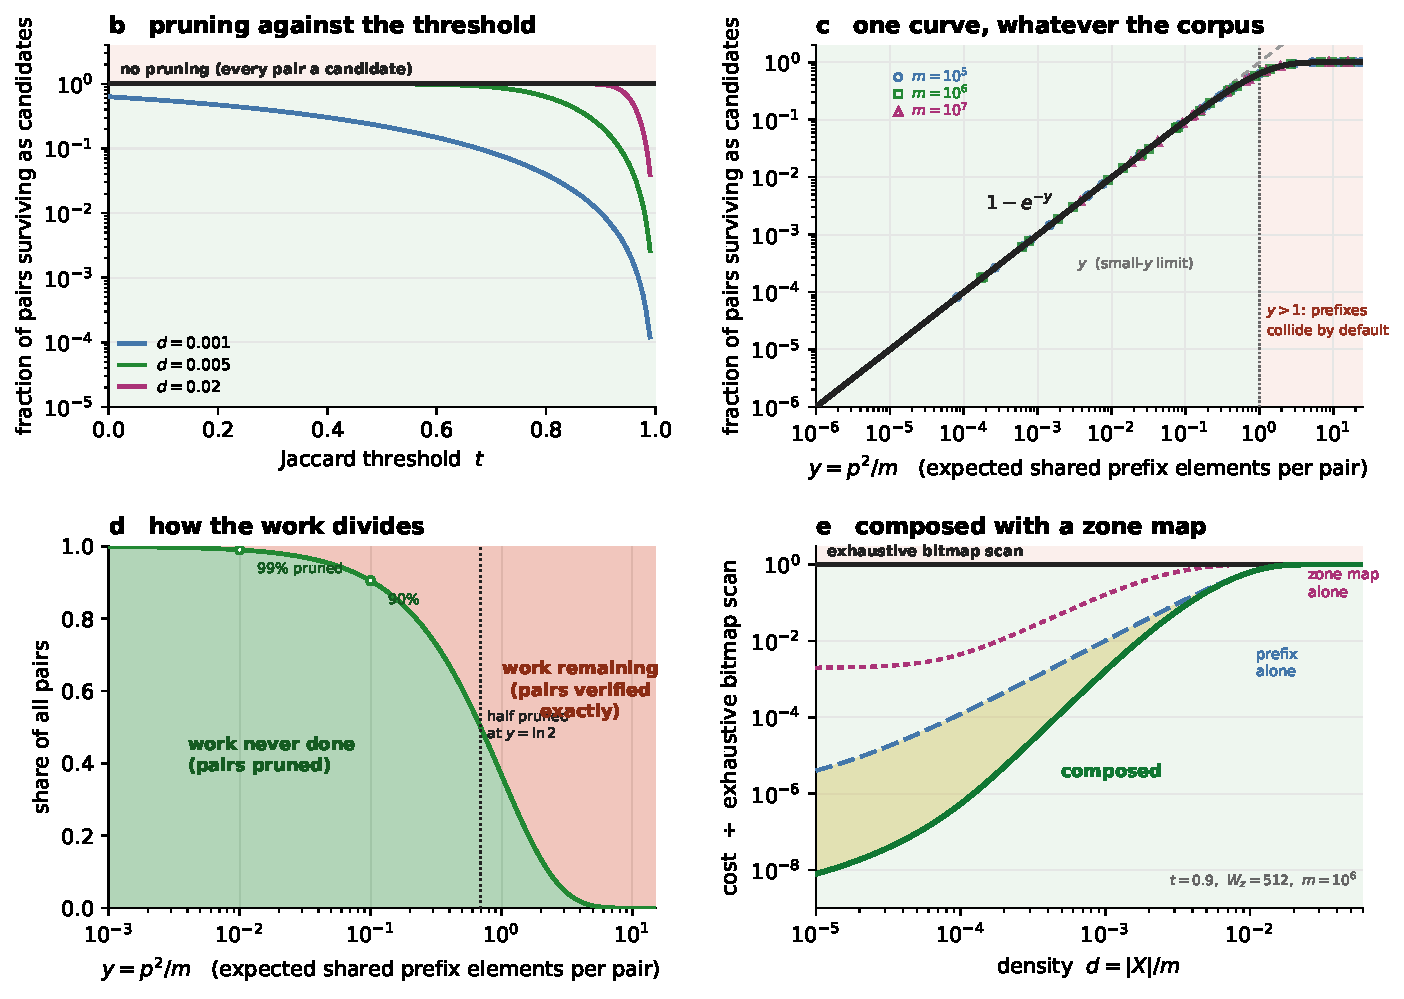
\includegraphics[width=\linewidth]{figures/fig3_prefix}
\caption{\textbf{Prefix filtering, analysed on the same terms --- and reducible to a single
variable.} Prefix filtering serves the opt-in thresholded mode, in which only pairs of Jaccard
similarity at least $t$ are reported. With elements in a global order and prefix length
$p(X) = |X| - \lceil t|X| \rceil + 1$, any qualifying pair must share an element between its
prefixes, so indexing prefixes alone answers the thresholded question exactly --- and unlike the
mechanisms of Fig.~\ref{fig:density-sweep}c--d it is candidate \emph{generation}: the quadratic pair
set is never enumerated. Reading key as in Fig.~\ref{fig:density-sweep}; an ordered series takes a
sequential ramp with its own marker or dash pattern.
\textbf{a}, How the rule works. Elements are laid out rarest first, hence the non-monotonic labels,
and each set's prefix (saturated) is its rarest $p(X)$ elements. Top: the prefixes share no element,
so the pair is discarded without computing any intersection. Bottom: one element appears in both,
marked in red because it is what commits the pair to exact verification.
\textbf{b}, Fraction of pairs surviving as candidates against the threshold, at universe $10^{6}$.
Prefix length falls as $t$ rises, so the filter that removes almost everything at a high threshold
removes almost nothing at a low one, and denser operands need a higher threshold to prune as hard.
\textbf{c}, All of that collapses onto one curve. For prefixes of length $p$ over a universe of $m$
the expected number of shared prefix elements per pair is $y = p^{2}/m$, and the surviving fraction
is exactly $1 - e^{-y}$ for scattered operands; markers are $(d,t,m)$ combinations drawn at random,
and lie on the curve by construction rather than by fit. For $y \ll 1$ the surviving fraction is $y$
itself; for $y > 1$ prefixes collide by default and the index is pure overhead. So $y$ --- not $t$,
and not density --- is what a selector should test.
\textbf{d}, The same as a division of labour: pairs never examined against pairs surviving to exact
verification. The two are equal at $y = \ln 2$.
\textbf{e}, Prefix filtering composed with a zone map. Unlike the two mechanisms of
Fig.~\ref{fig:density-sweep}c these \emph{do} compose --- their savings multiply, to within \nm{a
factor of 1.25 at the sparsest end, exactly elsewhere; analytic} --- because they act on different
waste and read different statistics. At $d = 10^{-3}$, $t = 0.9$ and $W_z = 512$ the composition
costs \nm{$\approx 0.17\%$, analytic} of an exhaustive bitmap scan, against $1.0\%$ for prefix
filtering alone and $16\%$ for a zone map alone.
Analytic throughout; no measured data, and like Fig.~\ref{fig:density-sweep} it models work rather
than time. \spec{Real corpora deviate in the same direction as elsewhere: frequency-ordered prefixes
concentrate rare elements, so real prefixes collide less than scattered ones of the same length and
the true curve lies below this one.}}
\label{fig:prefix}
\end{figure}

\subsection*{Supplementary Note 4: Derivation of the zone-map cost model and its crossings}
\label{sec:supp-note-4}

Relocated from Results, ``The cost of intersection is U-shaped in density,'' which points here for
the full derivation behind Fig.~\ref{fig:density-sweep}b--d: the null-model floor, the four counting
properties of a zone map (why it has a floor, why the leverage is large, why the advantage is flat
then erodes quadratically, and why it can be a liability), the crossing densities, and the
work-versus-time distinction.

Every panel of Fig.~\ref{fig:density-sweep} is the same argument applied to a different mechanism,
and it is worth stating that argument once. Each mechanism --- choosing a representation, consulting
a zone map, composing the two, and in the thresholded mode the prefix filter of
Supplementary Fig.~\ref{fig:prefix}
--- is a bet that the data deviates from randomness, and each comes with a closed-form null model
saying what the bet is worth if it does not. Fixing the density and placing elements independently is
the most pessimistic assumption available about \emph{arrangement}, and it is pessimistic in the same
direction for all of them: independent placement maximises the number of maximal runs a set has,
maximises the fraction of bins it occupies, and maximises the chance that two prefixes collide.
\textbf{The null model is therefore a floor and not a prediction.} Real structure can only move each
mechanism further into profit, and the size of that movement is exactly what the mechanism converts
into speed.

Two things a fixed design cannot do follow immediately, and they are the reason the selector is built
the way it is. A representation committed to at ingest cannot exploit the deviation, because it
commits before the deviation is knowable. A selector reading density alone cannot exploit it either,
because density is the very statistic the null model is built from: at a fixed density $d$ with
$k = dm$ elements the expected number of maximal runs is $k(m-k+1)/m$, but the actual number ranges
over every integer from one to $\min(k,\,m-k+1)$, so no single function of $d$ can track it. The
deviation is also \emph{one-sided} --- a real row can be arbitrarily cheaper than a random row of the
same density and at most about twice as expensive (Methods, ``What makes work avoidable'') --- which
is what makes it a resource
rather than a source of variance. Both readings point the same way: the statistic a selector consults
has to see arrangement, or be a direct measurement of the kernels themselves.

Four properties of the summary in Fig.~\ref{fig:density-sweep}b--c follow from counting alone, and
they are worth stating plainly because together they say what a summary can and cannot buy.

\emph{Why there is a floor, and where it is.} A zone map is a bitmap of bitmaps: one bit per bin of
$W_z$ positions, so $m/W_z$ bits against the row's $m$. Reading it therefore costs $1/W_z$ of reading
the row, and no pairing that consults a summary can cost less than reading that summary --- $0.195\%$
of a bitmap at $W_z = 512$. That is the floor, and it is a property of the bin width alone, not of the
data.

\emph{Why the leverage is so large.} The exchange rate is the same $W_z$: one summary bit decides the
fate of $W_z$ data bits, so a bin proved empty returns $W_z$ bits of work for the one bit spent
asking. This is why a coarser bin buys a deeper floor --- and, symmetrically, why it stops paying at a
lower density, since a wider bin is harder to leave empty.

\emph{Why the advantage is flat across the sparse range and then erodes quadratically.} A bin
survives only if \emph{both} operands occupy it, so the surviving fraction goes as the product of the
two occupancies. For clustered operands, where a run longer than a bin occupies exactly a $d$ fraction
of bins, that product is $d^2$, and the cost is $1/W_z + d^2\kappa$ with $\kappa$ the cost of a bin's
contents. The two terms are equal when $d^2\kappa = 1/W_z$; with $\kappa$ the cost of one run in a
bin, $\kappa = w/W_z$, this reduces to $d = 1/\sqrt{w} = 1/8$ --- \textbf{independent of the bin
width}. Below that density the summary term dominates and the advantage is constant; above it the
surviving-bin term dominates and the advantage decays as $d^{2}$. Changing $W_z$ moves the floor but
not the knee.

\emph{Why a summary can be a liability, and exactly when.} The floor cuts both ways, and the reason is
structural rather than a property of any one representation: \textbf{a summary is indexed by the
universe, while every compressed representation is indexed by the data}. The zone map costs $1/W_z$
of a bitmap whatever the operands contain, because its size is set by $m$. The cost of $\rS$, $\rR$
and $\rW$ is set instead by a quantity that shrinks with the set --- cardinality, run count, or
literal-and-fill count --- and each of those falls without limit as the operands sparsify. A fixed
cost and a vanishing one must cross. \textbf{Below that crossing, consulting a summary costs more than
the entire computation it was meant to shorten, and a zone map is worse than not having one.}

Where the crossing falls depends on which representation is being displaced, and one case fixes the
scale. A representation costing one word per element costs $w\,d$ of a bitmap, so it meets the
summary's $1/W_z$ at $d = 1/(wW_z) = 3.1\times10^{-5}$ for $w = 64$ and $W_z = 512$ (Methods,
Eq.~\eqref{eq:dlow}). At $d = 10^{-6}$ that representation costs $6.4\times10^{-5}$ of a bitmap while
the summary alone costs $1.95\times10^{-3}$, so consulting it does $31\times$ the work of simply
enumerating the operands. A run- or fill-based representation crosses at its own density, wherever its
run or word count falls below $m/W_z$, but that a crossing exists at all is generic.

This makes the gating two-sided, and for two unrelated reasons. A summary must be declined when the
operands are \emph{too dense}, because every bin is occupied and it proves nothing; and equally when
they are \emph{too sparse}, because it is then the largest object in the computation. It pays only
between those two bounds. \spec{The same fact appears in the storage measurements as
universe-proportional selector metadata dwarfing the data it describes; the time and space statements
of it are one phenomenon, and a guard on one is a guard on the other.}

The practical reading is that the sparse regime is not a narrow operating point. In the clustered
idealization --- the favourable edge of the band, where a run spans a whole bin --- the advantage is
the same at $d = 10^{-6}$ as at $d = 10^{-2}$: five orders of magnitude of density over which a
fixed-cost kernel does $512\times$ the work of one that consults a summary first. It is only above
$d = 1/8$ that the margin narrows at all, and even at $d \to 1$ a bitmap still does $7.9\times$ the
work.

All of the quantities above are counts of $64$-bit words touched, not times, and the distinction is
load-bearing rather than pedantic. A work model prices a summary that removes nothing at its own size,
$1/W_z$ of a bitmap, and that is a correct statement about words. It is not a statement about runtime:
a filtered scan gives up sequential access and hardware prefetch and pays an indirection and a branch
per bin, and the measured penalty for consulting a summary on operands it cannot help is far larger
than these panels charge --- \nm{worst-case speedup, filter applied unconditionally, which the work
model does not predict} against the $1.002\times$ overhead the work model allows, matching the
always-on-versus-gated contrast reported directly in Results, ``Selection must be hoisted, and
measured rather than modelled'' (Fig.~\ref{fig:selection-cost}c). That divergence is not a defect in
the derivation; it is the reason the gate is decided by measurement rather than by the model, and the
per-bin and per-word constants needed to convert these curves into time are given in Methods.

\subsection*{Supplementary Note 5: What repeats across a batch, and how each mechanism amortises it}
\label{sec:supp-note-5}

Relocated from Results, ``Selection must be hoisted, and measured rather than modelled,'' which points
here for the four quantities that repeat when a batch of pairs is run naively and how each is
amortised instead.

The contract is unchanged and the answer is identical, but batch amortisation requires many
operations rather than one, because what it removes is not work but \emph{repetition}. Four things
repeat when a batch is run naively, and each can be paid for once instead. Row metadata ---
cardinality, run count, occupancy summary --- is part of the representation, built at ingest and
amortised over every operation the set ever participates in rather than over any particular batch;
this is the same assumption Roaring's per-chunk container choice already makes, and it is stated here
once for the whole paper. A selection decision can be hoisted to a tile, so one decision serves a
block of pairs instead of one pair. Probe-and-commit pays to time a handful of operations and reuses
the verdict for the rest. And operand data loaded once can be paired against many, so its memory
traffic is amortised rather than repeated. In each case the same thing happens: the decision and the
metadata are amortised, and only the kernel work stays per operation (Supplementary
Fig.~\ref{fig:batch}b).
This is a regime rather than the setting. It applies wherever there are enough operations to share a
decision --- which is a property of a workload of any size, not an argument that anything must be
computed exhaustively --- and it is the regime in which the selection-cost measurements of the main
text were taken. The single-operation regime is reasoned instead from the cost of a decision read from
$O(1)$ metadata against the size of the operation it governs, and the asymmetry in evidence between
the two is stated here rather than left to be inferred.

Two mechanisms of that regime are drawn together in Supplementary Fig.~\ref{fig:batch}: an overlap
pre-filter that settles most of a pair set from summaries alone, and the way a decision's cost is
governed by the size of the operation it is made about.

\begin{figure}[!t]
\centering
% Column-postings tile pipeline. Body only; input inside a figure environment.
\definecolor{workc}{HTML}{EE6677}
\definecolor{avoidc}{HTML}{66CCEE}
\colorlet{zone}{black!20}

\tikzset{
  postcell/.style={draw=black!55, line width=0.35pt},
  postlabel/.style={font=\scriptsize, text=black!75},
  pipebox/.style={draw=black!60, rounded corners=1.2pt, align=center,
                 font=\scriptsize, inner sep=4pt, minimum height=9mm},
  pipearrow/.style={-{Latex[length=2mm]}, draw=black!65, line width=0.55pt},
}

\textbf{a}\par\vspace{0.6mm}
\resizebox{.96\linewidth}{!}{%
\begin{tikzpicture}[x=1mm,y=1mm]
  % Row-oriented incidence matrix.
  \node[postlabel, font=\scriptsize\bfseries, anchor=west] at (0,5)
    {row occupancy $A_{ib}$};
  \foreach \b in {0,...,3}{
    \node[postlabel] at (14+5*\b,1.7) {$b_{\b}$};}
  \foreach \i in {0,...,5}{
    \node[postlabel, anchor=east] at (10,-3-5*\i) {$X_{\i}$};}
  \foreach \bits [count=\i from 0] in {{1,0,0,1},{1,1,0,0},{0,0,1,0},
                                       {0,1,0,1},{1,0,0,0},{0,0,1,1}}{
    \foreach \bit [count=\b from 0] in \bits {
      \ifnum\bit=1 \def\fillc{zone}\else\def\fillc{white}\fi
      \draw[postcell,fill=\fillc] (11.5+5*\b,-5.5-5*\i) rectangle ++(5,5);}}

  % Explicit transpose into postings.
  \draw[pipearrow] (34,-13) -- (45,-13)
    node[midway,above,postlabel] {transpose};
  \node[postlabel, font=\scriptsize\bfseries, anchor=west] at (46,5)
    {column postings};
  \node[pipebox,fill=zone!65,minimum width=28mm] at (60,0) {$P_0=\{0,1,4\}$};
  \node[pipebox,fill=zone!65,minimum width=28mm] at (60,-10) {$P_1=\{1,3\}$};
  \node[pipebox,fill=zone!65,minimum width=28mm] at (60,-20) {$P_2=\{2,5\}$};
  \node[pipebox,fill=zone!65,minimum width=28mm] at (60,-30) {$P_3=\{0,3,5\}$};

  % Candidate matrix induced by the multi-row postings.
  \draw[pipearrow] (75,-13) -- (87,-13)
    node[midway,above,postlabel,align=center] {OR into\\candidate masks};
  \begin{scope}[shift={(90,0)}]
    \node[postlabel, font=\scriptsize\bfseries, anchor=west] at (0,5)
      {candidate pairs};
    \foreach \j in {0,...,5}{
      \node[postlabel] at (3+5*\j,1.7) {$\j$};}
    \foreach \i in {0,...,4}{
      \node[postlabel,anchor=east] at (-1,-3-5*\i) {$\i$};}
    \foreach \i/\js in {0/{1,3,4,5},1/{3,4},2/{5},3/{5}}{
      \foreach \j in \js {
        \draw[postcell,fill=workc!75] (0.5+5*\j,-5.5-5*\i) rectangle ++(5,5);}}
    \foreach \i/\js in {0/{2},1/{2,5},2/{3,4},3/{4},4/{5}}{
      \foreach \j in \js {
        \draw[postcell,dashed,fill=avoidc!25] (0.5+5*\j,-5.5-5*\i) rectangle ++(5,5);}}
    \node[postlabel,anchor=west] at (2,-33) {candidate};
    \draw[postcell,fill=workc!75] (-4,-35) rectangle ++(5,4);
    \node[postlabel,anchor=west] at (25,-33) {proved empty};
    \draw[postcell,dashed,fill=avoidc!25] (18,-35) rectangle ++(5,4);
  \end{scope}
\end{tikzpicture}}

\vspace{3mm}
\textbf{b}\par\vspace{0.6mm}
\resizebox{.96\linewidth}{!}{%
\begin{tikzpicture}[node distance=8mm and 8mm]
  \node[pipebox,fill=black!8] (gate) {online tile\\gate};
  \node[pipebox,fill=avoidc!18,right=of gate] (range) {sort by minimum\\and reject extents};
  \node[pipebox,fill=zone!55,right=of range] (transpose) {transpose row\\occupancy};
  \node[pipebox,fill=zone!55,right=of transpose] (compact) {retain multi-row\\postings};
  \node[pipebox,fill=workc!22,right=of compact] (resolve) {resolve unique\\candidate masks};
  \node[pipebox,fill=reprS!18,right=of resolve] (verify) {selected exact\\row cell};
  \draw[pipearrow] (gate) -- node[above,postlabel] {postings route} (range);
  \draw[pipearrow] (range) -- (transpose);
  \draw[pipearrow] (transpose) -- (compact);
  \draw[pipearrow] (compact) -- (resolve);
  \draw[pipearrow] (resolve) -- (verify);
  \node[pipebox,fill=reprB!10,below=10mm of transpose] (row) {row-pairing tournament\\for direct-route tiles};
  \draw[pipearrow] (gate.south) |- node[pos=.25,left,postlabel] {direct route} (row.west);
  \draw[pipearrow] (row.east) -| (verify.south);
\end{tikzpicture}}

\caption{\textbf{The batch regime: rejecting pairs wholesale, and paying for a decision once.}
Both mechanisms here need many operations rather than one, and what they remove is repetition.
\textbf{a}, An overlap pre-filter across a set of operands. The same occupancy idea as a zone map
(Fig.~\ref{fig:density-sweep}a) but at a coarser, chosen width and computed once per set, then
ANDed pairwise: shaded pair cells may overlap and are passed to a kernel, dashed cells are provably
disjoint and are answered without touching data. One pass over the summaries settles most of the
pair matrix. Note the distinction from prefix filtering (Supplementary Fig.~\ref{fig:prefix}), which
is candidate \emph{generation} and never enumerates the pair set at all.
\textbf{b}, Why the cost of a decision depends on what it governs. Each bar spends left-to-right
through one unit of useful work; the dashed rule marks that work with neither a decision nor a
filter. \emph{Deciding}: a single operation absorbs the decision easily, since it is read from
$O(1)$ metadata and the operation it governs is large; the same decision repeated for every
operation of a batch is a large fraction of the total, because each operation there is small; and
hoisting it to a tile --- deciding once, then committing --- restores the single-operation picture.
\emph{Filtering}: where bins are mostly empty a summary converts most of the work into skipped work;
where every bin is occupied it finds nothing to skip and its cost carries the bar past the rule.
The cost of deciding therefore scales inversely with how large the operation being decided about is,
which is why the two regimes need different policies and why every mechanism is gated rather than
always on. Schematic; no measured data.}
\label{fig:batch}
\end{figure}

\subsection*{Supplementary Note 6: Corpus provenance and inventory}
\label{sec:supp-note-6}

Supplementary Table~\ref{tab:corpus-inventory} gives full provenance and per-corpus statistics for
every corpus referenced anywhere in this paper, including the corpora scored only against an
all-bitmap baseline and never against CRoaring, which Table~\ref{tab:corpora} summarises in a single
row. It also records, for the two genomic corpora, which axis is treated as the universe under each
storage layout --- the distinction the main text draws in Results, ``Where the method does not
pay.''

% longtable is NOT a float and creates no group, so a bare \scriptsize here
% leaks into every following section. Keep it inside an explicit group.
% Start on a fresh page: the table is a full page of body, so letting it begin
% at the foot of the previous one emits an orphaned "(continued)" head with no
% rows under it.
\clearpage
\begingroup
\scriptsize
\setlength{\tabcolsep}{2.2pt}
% The document-wide \arraystretch{1.20} pushed this table one row past a full
% page, stranding that row behind two unrelated tables. Tightened so the whole
% inventory sits on one page.
\renewcommand\arraystretch{1.0}
% Corpus names are identifiers, so \seqsplit breaking them after one character
% is worse than a wrapped prose note. Width moved from the notes column to the
% name column; the total is unchanged, so the table cannot overflow.
\begin{longtable}{@{}p{3.7cm} l r r r r p{3.5cm}@{}}
\caption{\textbf{Corpora, provenance and statistics.} Every corpus referenced anywhere in this paper,
in four provenance groups used to assemble the benchmark set: \textbf{G1}, the twelve
\texttt{real-roaring-datasets} files CRoaring's own harness runs by default
\cite{chambi2016roaring,lemire2018roaring}; \textbf{G2}, five SNAP social/web graphs (Stanford Large
Network Dataset Collection) scored by neighbourhood-intersection density; \textbf{G3}, two genomic
corpora present for scoping rather than for the headline, included so a reader can judge whether the
benchmark set was chosen favourably; \textbf{G4}, KONECT graphs, UShER SARS-CoV-2, gnomAD and the
\texttt{msprime} coalescent-simulation series, added after the original survey. Density and mean
$|X_i|$ are corpus properties from the data loaders, not timing results. For the two G3 corpora,
\emph{universe} and \emph{rows} swap roles between layouts: \texttt{chr20.bin} is variant-major
(universe = 5{,}008 haplotypes, one row per variant site); \texttt{chr20\_hap.bin} is haplotype-major
(universe $\approx$ 1{,}048{,}576 sites, one row per haplotype) --- the layout dependence discussed in
the main text (Results, ``Where the method does not pay''). ---, not reported by the source.
\draftnote{All values provisional, pending the final measurement campaign.}}
\label{tab:corpus-inventory}\\
\toprule
Corpus & Group & Rows/sets & Universe $m$ & Mean $|X_i|$ & Density & Origin / notes \\
\midrule
\endfirsthead
\multicolumn{7}{l}{\textit{Table~\ref{tab:corpus-inventory} (continued)}} \\
\toprule
Corpus & Group & Rows/sets & Universe $m$ & Mean $|X_i|$ & Density & Origin / notes \\
\midrule
\endhead
\midrule \multicolumn{7}{r}{\textit{continued on next page}} \\
\endfoot
\bottomrule
\endlastfoot
\texttt{\seqsplit{census1881}} & G1 & \prov{200} & \prov{4{,}277{,}806} & \prov{5{,}019} & \prov{1.2e-3} & 1881 Canadian census, categorical attributes \\
\texttt{\seqsplit{census1881\_srt}} & G1 & \prov{200} & \prov{4{,}277{,}735} & \prov{3{,}404} & \prov{8.0e-4} & as above, rows sorted \\
\texttt{\seqsplit{census-income}} & G1 & \prov{200} & \prov{199{,}523} & \prov{34{,}610} & \prov{1.7e-1} & US census income (UCI ``Adult''-family), attributes \\
\texttt{\seqsplit{census-income\_srt}} & G1 & \prov{200} & \prov{199{,}523} & \prov{30{,}464} & \prov{1.5e-1} & as above, rows sorted \\
\texttt{\seqsplit{weather\_sept\_85}} & G1 & \prov{200} & \prov{1{,}015{,}367} & \prov{64{,}353} & \prov{6.3e-2} & September 1985 weather observations, binned attributes \\
\texttt{\seqsplit{weather\_sept\_85\_srt}} & G1 & \prov{200} & \prov{1{,}015{,}367} & \prov{80{,}540} & \prov{7.9e-2} & as above, rows sorted \\
\texttt{\seqsplit{wikileaks-noquotes}} & G1 & \prov{200} & \prov{1{,}353{,}179} & \prov{1{,}377} & \prov{1.0e-3} & WikiLeaks cable corpus, term/attribute postings \\
\texttt{\seqsplit{wikileaks-noquotes\_srt}} & G1 & \prov{200} & \prov{1{,}353{,}133} & \prov{1{,}440} & \prov{1.1e-3} & as above, rows sorted \\
\texttt{\seqsplit{uscensus2000}} & G1 & \prov{200} & \prov{36{,}974{,}578} & \prov{30} & \prov{8.1e-7} & US Census 2000; \textbf{sparsest and largest-universe G1 corpus} \\
\texttt{\seqsplit{dimension\_003}} & G1 & \prov{15{,}482} & \prov{3{,}866{,}847} & \prov{91} & \prov{2.4e-5} & Druid-derived dimension column \\
\texttt{\seqsplit{dimension\_008}} & G1 & \prov{5{,}240} & \prov{3{,}866{,}845} & \prov{347} & \prov{9.0e-5} & Druid-derived dimension column \\
\texttt{\seqsplit{dimension\_033}} & G1 & \prov{173} & \prov{3{,}866{,}847} & \prov{22{,}352} & \prov{5.8e-3} & Druid-derived dimension column \\
\addlinespace
\texttt{\seqsplit{as-skitter}} & G2 & \prov{1{,}696{,}415} & \prov{1{,}696{,}415} & \nm{n} & \prov{9.1e-6} & CAIDA skitter internet AS topology, 2005; undirected, symmetrized \\
\texttt{\seqsplit{wiki-Talk}} & G2 & \prov{2{,}394{,}385} & \prov{2{,}394{,}385} & \nm{n} & \prov{2.2e-5} & Wikipedia talk-page edits; directed; only 67{,}492 vertices have out-degree $\geq 2$ \\
\texttt{\seqsplit{soc-Pokec}} & G2 & \prov{1{,}632{,}803} & \prov{1{,}632{,}804} & \nm{n} & \prov{1.6e-5} & Pokec social network (Slovakia); directed; \textbf{lowest skew of the graphs} -- top 1\% of sets hold only 8.8\% of elements \\
\texttt{\seqsplit{com-LiveJournal}} & G2 & \prov{3{,}997{,}962} & \prov{4{,}036{,}538} & \nm{n} & \prov{5.1e-6} & LiveJournal friendship, ground-truth communities; undirected, symmetrized \\
\texttt{\seqsplit{com-Orkut}} & G2 & \prov{3{,}072{,}441} & \prov{3{,}072{,}627} & \nm{n} & \prov{2.7e-5} & Orkut social network; undirected, symmetrized; \textbf{largest input in this set} \\
\addlinespace
\texttt{\seqsplit{chr20.bin}} & G3 (scoping) & \nm{n} & \prov{5{,}008} & \nm{n} & \prov{3.5e-2} & 1/i site-frequency spectrum, 43.6\% singletons; variant-major, universe 626 bytes, L1-resident \\
\texttt{\seqsplit{chr20\_hap.bin}} & G3 (scoping) & \nm{n} & \prov{$\approx$1{,}048{,}576} & \nm{n} & \prov{3.1e-2} & haplotype-major; large universe but 3.1\% dense -- \textbf{nothing beats all-bitmap (0.93$\times$) at this density and layout} \\
\addlinespace
\texttt{\seqsplit{dbpedia-link}} & G4 & \prov{4{,}384{,}102} & \prov{18{,}268{,}993} & \prov{29.8} & \prov{1.63e-6} & KONECT \\
\texttt{\seqsplit{wikipedia\_link\_en}} & G4 & \prov{5{,}978{,}043} & \prov{11{,}206{,}012} & \prov{46.4} & \prov{4.15e-6} & KONECT \\
\texttt{\seqsplit{livejournal-groupmemberships}} & G4 & \prov{2{,}197{,}915} & \prov{7{,}489{,}074} & \prov{48.7} & \prov{6.50e-6} & KONECT, bipartite; universe \textbf{inflated} $\sim$2.3$\times$ (single id space for both columns; true member domain is 3{,}201{,}203) \\
\texttt{\seqsplit{usher\_sarscov2}} & G4 & \prov{29{,}411} & \prov{8{,}451{,}771} & \prov{15{,}769.3} & \prov{1.87e-3} & UCSC UShER SARS-CoV-2; mean dominated by near-universal variants (max 99.7\% carriers), \textbf{median only 404} \\
\texttt{\seqsplit{enwiki-categorylinks}} & G4 & \prov{2{,}165{,}205} & \prov{129{,}698{,}523} & \prov{102.3} & \prov{7.89e-7} & Wikimedia dumps; \textbf{largest universe, lowest density in the full set} \\
\texttt{\seqsplit{gnomad\_chr21\_exomes\_af1e-3}} & G4 & \prov{625{,}656} & \prov{1{,}461{,}894} & \prov{28.2} & \prov{1.93e-5} & gnomAD v4.1 \\
\texttt{\seqsplit{msprime\_10k}} & G4 (sim) & \prov{$\approx$42k} & \prov{2e4} & \prov{1{,}887} & \prov{9.4e-2} & msprime coalescent simulation; out of target regime \\
\texttt{\seqsplit{msprime\_100k}} & G4 (sim) & \prov{$\approx$51k} & \prov{2e5} & \prov{15{,}720} & \prov{7.9e-2} & as above; out of target regime \\
\texttt{\seqsplit{msprime\_1M}} & G4 (sim) & \prov{$\approx$15.6k} & \prov{2e6} & \prov{136{,}288} & \prov{6.8e-2} & as above; out of target regime \\
\end{longtable}
\endgroup

\subsection*{Supplementary Note 7: Selector-metadata overhead and storage cost}
\label{sec:supp-note-7}

Storage is a reported trade-off rather than an objective this paper optimizes for. The two tables
below separate the two costs that the main text keeps apart. Supplementary Table~\ref{tab:metadata}
gives the metadata the selector itself needs, per row and against the data it describes; it is the
evidence behind the third boundary named in Results, ``Where the method does not pay,'' and it shows
that the rank index and zone map are sized by the universe rather than by the row.
Supplementary Table~\ref{tab:storage} gives the cost of the chosen data representation alone, with
that metadata excluded, so the two are never conflated.

\begin{table}[!t]
\footnotesize
\setlength{\tabcolsep}{6pt}
\renewcommand\arraystretch{1.05}
\centering
\caption{\textbf{Selector metadata is universe-proportional, and that is a defect.} The rank index
and zone map are constructed unconditionally, and both scale with \textbf{universe}, not
cardinality. \textbf{Meta B/row} and \textbf{data B/row} are bytes of selector metadata and bytes of
the chosen data representation, per row; \textbf{ratio} is meta:data. On
\texttt{enwiki-categorylinks} that is \prov{4} MB of selector metadata attached to \prov{155} bytes
of data -- a \prov{26{,}312$\times$} overhead. The complement representation already carries a guard,
built only when $2n > \text{universe}$; rank and occupancy carry none. Rows on which metadata exceeds data by more than $10^{3}\times$ are bold. This is a known, unfixed
property of the current implementation rather than a design choice, and it is why bitmap-bearing
measurements elsewhere in this paper are restricted to small row counts on the large-universe
corpora. \draftnote{All values provisional, pending the final measurement campaign.}}
\label{tab:metadata}
\begin{tabular}{@{}l r r r r@{}}
\toprule
Corpus & Universe $m$ & Meta B/row & Data B/row & Ratio (meta:data, $\times$) \\
\midrule
\texttt{census-income} & \prov{199{,}523} & \prov{6{,}335} & \prov{13{,}344} & \prov{0.5} \\
\texttt{weather\_sept\_85} & \prov{1{,}015{,}367} & \prov{32{,}031} & \prov{54{,}497} & \prov{0.6} \\
\texttt{census1881} & \prov{4{,}277{,}806} & \prov{134{,}784} & \prov{18{,}774} & \prov{7.2} \\
\texttt{as-skitter} & \prov{1{,}696{,}415} & \prov{53{,}479} & \prov{49} & \textbf{\prov{1{,}083}} \\
\texttt{dbpedia-link} & \prov{18{,}268{,}993} & \prov{575{,}415} & \prov{113} & \textbf{\prov{5{,}051}} \\
\texttt{enwiki-categorylinks} & \prov{129{,}698{,}523} & \prov{4{,}084{,}799} & \prov{155} & \textbf{\prov{26{,}312}} \\
\bottomrule
\end{tabular}
\end{table}

\begin{table}[!t]
\footnotesize
\setlength{\tabcolsep}{5pt}
\renewcommand\arraystretch{1.05}
\centering
\caption{\textbf{Storage cost, bits per value, data and metadata separated.} Reported the way the
Roaring papers report it \cite{lemire2016roaring}, so corpora of different cardinality are
comparable. \textbf{Metadata is excluded from every column here}: the zone map and rank index are
what the selector needs to \emph{choose} a representation, not a representation themselves, and
folding them into a data column would hide the cost of the mechanism this paper adds
(Supplementary Table~\ref{tab:metadata}). \textbf{Best} is the minimum of the four representation columns, per
corpus, and is set in bold in every row for that reason. Bitmap costs are given in scientific notation throughout, one notation down the column. On dense corpora the numbers are Roaring-comparable ($3$--$7$ bits/value); on sparse corpora
a dense bitmap costs $10^{3}$--$10^{6}$ bits/value, the storage statement of the same fact the timing
tables make: a bitmap over a large sparse universe is not a compression scheme, it is a liability.
\draftnote{All values provisional, pending the final measurement campaign.}}
\label{tab:storage}
\begin{tabular}{@{}l r r r r r r@{}}
\toprule
Corpus & Universe $m$ & \multicolumn{5}{c}{Bits per value} \\
\cmidrule(lr){3-7}
& & Bitmap & Array & Runs & EWAH & \textbf{Best} \\
\midrule
\texttt{census-income} & \prov{199{,}523} & \prov{5.77e0} & \prov{32.00} & \prov{20.73} & \prov{3.86} & \textbf{\prov{3.08}} \\
\texttt{msprime\_100k} & \prov{200{,}000} & \prov{1.26e1} & \prov{32.00} & \prov{31.88} & \prov{5.29} & \textbf{\prov{4.44}} \\
\texttt{weather\_sept\_85} & \prov{1{,}015{,}367} & \prov{1.58e1} & \prov{32.00} & \prov{30.06} & \prov{7.87} & \textbf{\prov{6.77}} \\
\texttt{usher\_sarscov2} & \prov{8{,}451{,}771} & \prov{1.08e3} & \prov{32.00} & \prov{2.04} & \prov{4.06} & \textbf{\prov{2.02}} \\
\texttt{wikileaks-noquotes} & \prov{1{,}353{,}179} & \prov{9.83e2} & \prov{32.00} & \prov{11.36} & \prov{19.46} & \textbf{\prov{10.64}} \\
\texttt{census1881} & \prov{4{,}277{,}806} & \prov{8.52e2} & \prov{32.00} & \prov{58.86} & \prov{43.79} & \textbf{\prov{29.92}} \\
\texttt{as-skitter} & \prov{1{,}696{,}415} & \prov{1.26e5} & \prov{32.00} & \prov{47.13} & \prov{77.72} & \textbf{\prov{29.26}} \\
\texttt{wikipedia\_link\_en} & \prov{11{,}206{,}012} & \prov{2.68e5} & \prov{32.00} & \prov{46.21} & \prov{72.90} & \textbf{\prov{28.27}} \\
\texttt{dbpedia-link} & \prov{18{,}268{,}993} & \prov{6.38e5} & \prov{32.00} & \prov{56.38} & \prov{101.63} & \textbf{\prov{31.84}} \\
\texttt{uscensus2000} & \prov{36{,}974{,}578} & \prov{1.24e6} & \prov{32.00} & \prov{57.78} & \prov{91.89} & \textbf{\prov{31.98}} \\
\texttt{enwiki-categorylinks} & \prov{129{,}698{,}523} & \prov{3.33e6} & \prov{32.00} & \prov{62.72} & \prov{113.23} & \textbf{\prov{31.85}} \\
\bottomrule
\end{tabular}
\end{table}

\subsection*{Supplementary Note 8: Formal treatment of work avoidance --- full proofs}
\label{sec:supp-note-8}

Methods (``What makes work avoidable'') states each result of this development as an equation with
its hypotheses and a pointer here. This note supplies the proof, the worked numerical checks and the
secondary results that support but do not themselves state a numbered result in Methods. Notation
follows Methods throughout: $A,B\subseteq[0,m)$, $a=|A|$, $b=|B|$, $d_A=a/m$, $d_B=b/m$, word width
$w$, effective sparsity $s_X=\min(d_X,1-d_X)$, $s=\min(s_A,s_B)$. For a representation $\rho$ and a
set $X$, $\kappa_\rho(X)$ is the number of stored items a kernel must touch to traverse $X$ in that
representation --- $\lceil m/w\rceil$ words for \rB, $|X|$ for \rS, the run count $r(X)$ for \rR, and
literal-word count plus fill-group count $\ell(X)+g(X)$ for \rW. All costs below are counts of stored
items or of elementary operations, never a time; the constants that convert one to the other are
measured, not derived, and are given in Methods under ``Benchmark protocol and cache-residency
statement''.

\paragraph*{Proof of Eq.~\eqref{eq:interval} (the Fr\'echet interval) and Eq.~\eqref{eq:width} (its width).}
Upper bound: $A\cap B\subseteq A$ and $A\cap B\subseteq B$, so $|A\cap B|\le\min(a,b)$. Lower bound:
$|A\cup B|=a+b-|A\cap B|\le m$, so $|A\cap B|\ge a+b-m$; together with $|A\cap B|\ge0$ this gives the
stated interval. Every integer $t$ in the range is attained: take $A=[0,a)$ and $B=[a-t,\,a-t+b)$,
so that $A\cap B=[a-t,a)$ has size $t$. The construction is legal because $t\le a$ gives $a-t\ge0$,
$t\ge a+b-m$ gives $a-t+b\le m$, and $t\le b$ makes $[a-t,a)\subseteq B$.

For the width, $\min(a,b)-\max(0,a+b-m)=\min(a,b)+\min(0,m-a-b)=\min\big(\min(a,b),\,\min(a,b)+m-a-b\big)$,
and $\min(a,b)+m-a-b=m-\max(a,b)$, so the width is $\min\big(\min(a,b),\,m-\max(a,b)\big)=\min(a,b,m-a,m-b)$.
Grouping the four terms in pairs, $\min\big(\min(a,m-a),\,\min(b,m-b)\big)=\min(m\,s_A,m\,s_B)=m\,s$.
The number of feasible answers is $m\,s+1$, so a cardinality-only view of a pair leaves
$\log_2(m\,s+1)$ bits of the answer unresolved. The four terms $a,b,m-a,m-b$ are exactly the sizes of
the four lists $A,B,A^c,B^c$ one could enumerate, so the residual uncertainty is the size of the
smallest of them --- not a coincidence, since Eq.~\eqref{eq:headroom}'s proof below shows the
smallest of those four lists is precisely what an exact algorithm enumerates to answer the query.

\emph{The pigeonhole floor.} The lower bound of Eq.~\eqref{eq:interval} lifts off zero exactly when
$d_A+d_B>1$, giving $|A\cap B|\ge(d_A+d_B-1)m$; equivalently, by inclusion--exclusion on complements,
$|A\cap B|=a+b-m+|A^c\cap B^c|$, so the floor is the case $A^c\cap B^c=\varnothing$: the complements
can be at most disjoint. At $d_A=d_B=0.51$ the floor is $(2\cdot0.51-1)m=0.02m$ --- the factor is two,
so $51\%$ density forces $2\%$ of the universe to overlap, not $1\%$; as a fraction of either operand
it is $2-1/d\approx3.92\%$. Above $d=\tfrac12$ the floor rises at $2m$ per unit density while the
ceiling $\min(a,b)=dm$ rises at $m$, so the width $m(1-d)$ shrinks at the constant rate $m$ per unit
density --- consistent with $m(1-d)=m\,s$ for $d\ge\tfrac12$.

\paragraph*{Proof of Eq.~\eqref{eq:headroom} (the headroom).}
$\kappa(\rB)=\lceil m/w\rceil$ for every $X$ by definition: a dense bitmap stores $m$ bits whatever
they contain, so $\cell{\rB}{\rB}$ performs $\lceil m/w\rceil$ word AND-plus-popcount operations for
every pair independently of $a$, $b$, of structure and of the answer. This is not a defect of any
implementation; \rB\ is the only member of the matrix whose descriptor length is a function of the
universe alone.

Suppose each operand $X$ is available as a bitmap \emph{and} as a sorted array of whichever of $X$,
$X^c$ is the smaller --- $\Theta(m\,s_X)$ of extra space, decided from $a,b,m$ in $O(1)$. No rank
index is required for what follows; that enters separately, below. Without a stored complement array,
enumerating $X^c$ from the bitmap costs $\Theta(m/w+(m-a))$, whose first term is already $\kappa(\rB)$
--- so the dense arm of the argument genuinely requires the complement to be materialised, not derived
on the fly. Then $|A\cap B|$ is computed in $O(m\,s)$ constant-time membership probes, by four cases,
one per term of $\min(a,b,m-a,m-b)$: if $U=a$, enumerate $A$'s $a$ positions and probe each into $B$'s
bitmap ($a$ probes); if $U=b$, symmetric; if $U=m-a$, enumerate $A^c$ and recover
$|A\cap B|=b-|A^c\cap B|$ ($m-a$ probes); if $U=m-b$, symmetric via $|A\cap B|=a-|A\cap B^c|$. Each
case is $O(1)$ arithmetic plus $U$ probes. Two of the four cases require the complement view, which is
why \rC\ is part of the design and not an afterthought for the dense tail: without it the achievable
cost is $\min(a,b)$, which is $\Theta(m)$ at high density, and the dense arm of the U does not exist.

Comparing descriptor items touched, $\kappa(\rB)/U=\lceil m/w\rceil/(m\,s)$. Taking $w\mid m$ (true of
the implementation, which pads to a whole number of words) this is exactly $1/(w\,s)$; otherwise read
it as $\ge$ with an additive $w/m$ term (relative error at $m=1000,w=64$ is $2.4\%$, at $m=65$ it is
$97\%$; nothing downstream changes). The ratio exceeds one whenever $s<1/w$ and is unbounded as
$s\to0$. \textbf{What this does and does not assert:} it asserts that a specific, exact, correct
algorithm exists whose cost is $m\,s$ items where $\cell{\rB}{\rB}$ spends $m/w$ items, and that the
ratio between the two achieved costs diverges. It does \emph{not} assert that $m\,s$ is a lower bound
on the work any algorithm must do (``Why the interval width is not a lower bound on work'', below);
both quantities compared are achieved, neither is a floor.

\emph{The crossover heuristic.} Converting to time needs two measured constants: the cost of a random
probe into a bitmap, $c_p$, and the cost of a vectorised AND-plus-popcount word, $c_w/V$. Equating the
two costs gives the crossover $s^*=c_w/(c_p\,w\,V)$ --- an explicitly constant-factor, not asymptotic,
argument, and the only quantitative prediction of this kind in this note.

\paragraph*{Proof of Eq.~\eqref{eq:rank} (the rank-index bridge).}
This is the only result here that converts a descriptor \emph{length} into an \emph{operation count};
every other result in this note is a fact about storage. Let $A$ be a bitmap carrying an $O(1)$ rank
index, $\mathrm{rank}_A(i)=|A\cap[0,i)|$, and $B$ a run container with maximal runs $\{[u_i,v_i)\}$,
$i=1,\dots,r$. The runs partition $B$, so $A\cap B$ is the disjoint union of $A\cap[u_i,v_i)$, and
$|A\cap[u_i,v_i)|=\mathrm{rank}_A(v_i)-\mathrm{rank}_A(u_i)$ by the definition of rank. Summing over
the $r$ runs gives Eq.~\eqref{eq:rank}, computed in exactly $2r$ rank lookups and $2r-1$ additions ---
independent of $m$, of $|A|$, of $|B|$ and of the run lengths $v_i-u_i$: a run of any length is priced
as a run of length one, because the kernel never looks inside it. Symmetrically, $\cell{\rR}{\rR}$ by
simultaneous merge of two sorted run lists costs $O(r_A+r_B)$ with no rank index needed, since the
merge never inspects a position inside a run. This is what makes a run count a cost parameter and not
merely a storage parameter; it converts descriptor length into operation count, not into time, since
per-operation constants still differ across cells.

\paragraph*{Proofs for Eq.~\eqref{eq:expected} (expected descriptor lengths under a null model).}
Model: each position of $[0,m)$ is set independently with probability $d$ (Bernoulli), and $w\mid m$
so every word carries $w$ live bits. The \rB\ and \rS\ rows are exact and not asymptotic statements at
all: $\mathbb{E}\,\kappa(\rB)=\lceil m/w\rceil$ trivially, and $\mathbb{E}\,\kappa(\rS)=m\,d$ by
linearity of expectation over the $m$ indicator variables. For $\rC\!\circ\!\rho$, substitute $1-d$ for
$d$, since complementation is an involution on density.

\emph{Run count.} A maximal run of ones begins at position $i$ iff $x_i=1$ and ($i=0$ or $x_{i-1}=0$).
Summing the indicator expectations over $i=0,\dots,m-1$ gives the exact Bernoulli
$\mathbb{E}[r]=d+(m-1)d(1-d)$; under the fixed-cardinality model (uniform random $k$-subset) the same
argument gives the exact $\mathbb{E}[r]=k(m-k+1)/m$. Both equal $m\,d(1-d)(1+O(1/m))$, whose
leading-order form in $s=\min(d,1-d)$ is $m\,s(1-s)$, the form used in Eq.~\eqref{eq:expected}.
\textbf{The sandwich is exact, not merely leading-order:} writing $p_0=(1-d)^w$ is not needed here, but
the two exact forms bound each other by
\begin{equation}
\tfrac12\,m\,s \;\le\; \mathbb{E}\,\kappa(\rR) \;\le\; m\,s+1,
\label{eq:s3-corA-sandwich}
\end{equation}
since fixed-cardinality $\mathbb{E}[r]=m\,s(1-s)+d$ and Bernoulli $\mathbb{E}[r]=m\,s(1-s)+d^2$ both
exceed $m\,s$ marginally at the dense corner ($m=64,k=57$ gives $\mathbb{E}[r]=7.125$ against
$m\,s=7$; the worst ratio $\mathbb{E}[r]/(m\,s)$ tends to $2$). This corrects an earlier form of the
sandwich that omitted the $+1$ and is violated by $38$ cases near $d\to1$ without it.

\emph{Fill-compressed stream.} Let $p_0=(1-d)^w$, $p_1=d^w$ be the probabilities that a $w$-bit word is
all-zero or all-one, and $n=m/w$. Words are independent because they cover disjoint bit ranges (this
is where $w\mid m$ is used). Dirty (literal) words: $\mathbb{E}[\ell]=n(1-p_0-p_1)$. Fill groups: a
maximal block of consecutive all-$v$ words begins at word $j$ iff word $j$ is all-$v$ and ($j=0$ or
word $j-1$ is not all-$v$), so $\mathbb{E}[g_v]=p_v+(n-1)p_v(1-p_v)$ exactly. Summing over
$v\in\{0,1\}$,
\begin{equation}
\mathbb{E}[\ell+g] \;=\; n(1-p_0-p_1) + p_0+(n-1)p_0(1-p_0) + p_1+(n-1)p_1(1-p_1)
\;=\; n-(n-1)(p_0^2+p_1^2),
\label{eq:s3-wah-exact}
\end{equation}
which to leading order in $n$ is $n[1-p_0^2-p_1^2]$, matching Eq.~\eqref{eq:expected}'s form
$(m/w)[1-(1-s)^{2w}-s^{2w}]$ (the exact form exceeds the leading-order one by at most
$p_0^2+p_1^2\le2$ words, immaterial at any $n$ of interest). The encoding must compress both all-zero
\emph{and} all-one fills for the symmetry claims below to hold; an encoder compressing only zero fills
is not complement-symmetric. \textbf{Sparse limit.}
$(1/w)[1-(1-s)^{2w}-s^{2w}]\to2s$ as $s\to0$, so under the null model \rW\ costs about \emph{twice} \rS\
in the sparse tail, not the same --- the reason \rW\ never appears on the cost envelope in either tail.

\paragraph*{Complement symmetry (Proposition 9, supporting the paragraph ``the deviation, which is the
contribution'').}
$\kappa(\rS)(X^c)=m-\kappa(\rS)(X)$: \rS\ is \emph{not} complement-symmetric, which is why the \rC\
strategy exists. $\kappa(\rB)(X^c)=\kappa(\rB)(X)$ trivially. \rR\ is complement-symmetric by
construction, because runs of ones and runs of zeros alternate along $[0,m)$, so
$|r(X^c)-r(X)|\le1$; the sign is not a two-sided uncertainty for a given set, it is determined by
boundary membership, exactly $r(X^c)=r(X)-1+\mathbb{1}[0\notin X]+\mathbb{1}[m-1\notin X]$:

\begin{center}
\begin{tabular}{ccc}
\toprule
$0\in X$ & $m-1\in X$ & $r(X^c)-r(X)$ \\
\midrule
no & no & $+1$ \\
no & yes & $0$ \\
yes & no & $0$ \\
yes & yes & $-1$ \\
\bottomrule
\end{tabular}
\end{center}

Degenerate cases obey it: $X=\varnothing$ gives $r=0$, $r(X^c)=1$; $X=[0,m)$ gives $r=1$, $r(X^c)=0$.
This is why $\cell{\rR}{\rR}$ wins the dense tail with no complement machinery: $\rR$'s descriptor
length is nearly invariant under complementation, while $\rS$'s is not, which is exactly why the
array-based cells need an explicit complement view and the run-based ones do not.
$\kappa(\rW)(X^c)=\kappa(\rW)(X)$ \emph{exactly, provided $w\mid m$}: complementing every word maps
all-zero words to all-one words and back and maps dirty words to dirty words, leaving the
literal/fill partition untouched. This fails when $w\nmid m$: a zero-padded tail word that is
all-ones over the live bits is not all-ones over the padded word, so complementation moves it between
the literal and fill classes.

\paragraph*{Proof of the U-shape as a theorem of the null model (supporting ``what randomness would
predict'').}
Each leading-order entry of Eq.~\eqref{eq:expected} is, as a function of $s$, either constant (\rB) or
strictly increasing on $[0,\tfrac12]$: best-of-$\rS/\rC\!\circ\!\rS$ is $m\,s$, increasing; \rR\ is
$m\,s(1-s)$, and $\mathrm{d}/\mathrm{d}s[s(1-s)]=1-2s>0$ for $s<\tfrac12$; \rW\ is
$(m/w)[1-(1-s)^{2w}-s^{2w}]$, with derivative $(m/w)\cdot2w[(1-s)^{2w-1}-s^{2w-1}]>0$ for $s<\tfrac12$.
Each is symmetric about $d=\tfrac12$ by construction. \textbf{This is a statement about the
leading-order forms, not the exact ones}: the exact Bernoulli $\mathbb{E}[r]=d+(m-1)d(1-d)$ is not
itself a function of $s$ (at $m=1000$ it is $90.01$ at $d=0.1$ and $90.81$ at $d=0.9$, a gap of
$1-2d$, and its maximum sits at $d=\tfrac12+1/(2(m-1))$ rather than at $d=\tfrac12$), while
$\mathbb{E}\,\kappa(\rW)$ \emph{is} exactly a function of $s$, since $(1-d)^{2w}+d^{2w}$ is symmetric
under $d\mapsto1-d$. Nothing downstream depends on the choice.

By Eq.~\eqref{eq:s3-corA-sandwich}, the four compressed representations agree to within a constant
factor under the null model: $\rS$-with-complement costs $m\,s$, $\rR$ costs between $\tfrac12ms$ and
$ms+1$, and $\rW$ costs about $2ms$ in the sparse tail while saturating at $m/w$. Selection
\emph{among} $\{\rS,\rC\!\circ\!\rS,\rR,\rW\}$ therefore buys at most a constant under randomness ---
randomness gives run containers nothing over sorted arrays. \rB\ is the exception and the exception is
the entire point: it is a member of the matrix and its expected cost is $m/w$ at every density, so the
spread across the full matrix is $(m/w)/(m\,s)=1/(w\,s)$ (Eq.~\eqref{eq:headroom}), which is unbounded.
At $s=10^{-6}$ the ratio of the most to the least expensive representation in the matrix exceeds
$10^4$. What collapses under randomness is the choice among the compressed representations; what does
not collapse is the choice between the bitmap and the rest. Correspondingly it is the \emph{envelope},
not every cell, that is $\Theta(\min(m/w,m\,s))$ --- $\kappa(\rB)$ is $m/w$ regardless. The crossover of
that envelope sits at $w\,s\approx1$, i.e.\ $s^*\approx1/w$, about $1.6\%$ for $w=64$ before per-item
constants. \textbf{The U-shape is a genuine theorem of the null model and of the bitmap's flatness. It
is not a property of the method, and the method is not in the business of reproducing it} --- on real
data the representations deviate below the null without limit, and that deviation, not the U itself, is
the contribution (next).

\paragraph*{Proof that density is not a sufficient statistic for cost (the deviation, supporting
Eq.~\eqref{eq:expected} and the impossibility argument).}
Fix $m$ and $d\le\tfrac12$, $k=dm$. Over the sets of density exactly $d$: $\kappa(\rB)$ and
$\kappa(\rS)$ are constants, functions of $(m,k)$ alone; $\kappa(\rR)$ ranges over \emph{every}
integer in $[1,\min(k,m-k+1)]$; $\kappa(\rW)$ ranges from $O(1)$ to $\Theta(\min(k,m/w))$. Two explicit
families witness the extremes. $X_{\mathrm{block}}=[0,k)$ has one run, $r=1$, and its words are one
all-one fill flanked by all-zero fills, so $\kappa(\rW)=O(1)$. For the spread extreme, take
\begin{equation}
X_{\mathrm{spread}} \;:=\; \{\,i\,\lfloor m/k\rfloor \;:\; 0\le i<k\,\},
\label{eq:s3-xspread}
\end{equation}
which has $|X_{\mathrm{spread}}|=k$ \emph{exactly} (the largest element is $(k-1)\lfloor m/k\rfloor<m$)
--- unlike the naive candidate ``every $\lceil1/d\rceil$-th position'', which has density $k=dm$ only
when $1/d$ is an integer and is not used here for that reason. The stride $\lfloor m/k\rfloor\ge2$
whenever $k\le m/2$, so every element of $X_{\mathrm{spread}}$ is isolated and $r=k$. For $\kappa(\rW)$:
every $w$-bit word contains at least one element iff the stride is $\le w$, i.e.\ iff $d\gtrsim1/w$, in
which case every word is dirty and $\kappa(\rW)=m/w$; otherwise the $k$ elements fall in distinct
words, giving $k$ dirty words separated by $\Theta(k)$ fill groups, $\kappa(\rW)=\Theta(k)$. For the
intermediate run counts, choose any composition of $k$ into $r$ parts (the run lengths) and any
distribution of the $m-k$ zeros into the $r+1$ gaps with the $r-1$ internal gaps non-empty; this is
feasible iff $r\le k$ and $r\le m-k+1$, exactly the claimed range (a run needs at least one element,
and $r$ runs need at least $r-1$ separating gaps).

\emph{The worked case.} $m=10^6$, $A=[0,5\times10^5)$, $B=[2.5\times10^5,7.5\times10^5)$. Both operands
sit at density exactly $\tfrac12$ --- the worst point of Eq.~\eqref{eq:width}, where cardinality alone
leaves $500{,}001$ feasible answers and the null model of Eq.~\eqref{eq:expected} predicts $m/4=250{,}000$
runs apiece. Both in fact have one run. $\cell{\rB}{\rR}$ with a rank index (Eq.~\eqref{eq:rank})
answers the pair in \emph{two rank lookups}; $\cell{\rB}{\rB}$ spends $15{,}625$ word operations to
reach the same number. Nothing about the density says which situation a selector is in.

\emph{The structure ratio.} Define $\sigma_\rho(X):=\mathbb{E}_{\mathrm{null}(d)}[\kappa_\rho]/\kappa_\rho(X)$,
against the \emph{fixed-cardinality} null throughout ($\mathbb{E}[r]=k(m-k+1)/m$), which conditions on
the observable $k$ and is exact; it differs from the Bernoulli form by $O(1)$ and nothing depends on
the choice. $\sigma_\rho\equiv1$ identically for \rB\ and \rS. At every density,
\begin{equation}
\sigma_\rR(X) \;\ge\; \frac{\max(k,\,m-k+1)}{m} \;=\; \max\big(d,\;1-d+\tfrac1m\big) \;\ge\; \tfrac12,
\label{eq:s3-p10}
\end{equation}
with equality only for the maximally scattered set, and $\sigma_\rR$ is unbounded above, reaching
$\Theta(m)$ on $X_{\mathrm{block}}$. \emph{Proof.}
$\sigma_\rR=\mathbb{E}[r]/r\ge\mathbb{E}[r]/r_{\max}$ with $r_{\max}=\min(k,m-k+1)$ and
$\mathbb{E}[r]=k(m-k+1)/m$; since $xy/\min(x,y)=\max(x,y)$, the ratio is $\max(k,m-k+1)/m$, which
exceeds $\tfrac12$ because $k+(m-k+1)=m+1>m$ forces the larger term above $m/2$. This is stronger than
a $d\le\tfrac12$-only bound: the restricted form $1-d+1/m$ degenerates to $0.002$ at $d=0.999$, a
spurious $500\times$ worst case, where the true bound is $\sigma_\rR\ge0.999$. Read as a sentence:
\textbf{real data can be arbitrarily cheaper than random data at the same density, and at most about
twice as expensive.}

\emph{The impossibility (Corollary B), stated at the strength it is actually proved.} Any selector
whose input is $d$ (or $a$, $b$, or any function of them) evaluates one fixed function $f(d)$ on every
row of that density; by the range above, $\kappa(\rR)$ takes every value in $[1,k]$ at $d=k/m$, so
$f(d)$ mis-predicts $\kappa(\rR)$ by an unbounded factor on some rows at every density, and no such
selector can distinguish $X_{\mathrm{block}}$ from $X_{\mathrm{spread}}$. Two consequences, and the
line between what is proved and what is measured must be drawn precisely. (i) A fixed representation
cannot exploit $\sigma$, since it commits before $\sigma$ is knowable. (ii) A density-only \emph{cost
model} cannot exploit $\sigma$ either, since it is a function of $d$ and the impossibility applies to it
verbatim --- but it does \emph{not} follow that such a model is worse than making no selection at all:
whether a mis-prediction costs more than a fixed default depends on which cell the wrong prediction
picks and that cell's actual cost, neither of which is modelled here. The regret comparison in
Results, ``Selection must be hoisted, and measured rather than modelled''
(Fig.~\ref{fig:selection-cost}b), is a measurement of that question, not a derivation of it.
What \emph{is} licensed is narrower and still strong: the
proved statement rules out one class of selector --- those reading only cardinality --- and does not
choose among the survivors. A run count or a zone-map occupancy count is $O(1)$ metadata that sees
$\sigma$ perfectly and can perfectly well be fed to a model; probe-and-commit is a different survivor.
The theory says only: gate selection on a statistic that sees structure rather than on cardinality.
Whether that statistic feeds a structural model or a direct measurement of the candidate kernels is
settled by measurement, not derived here.

\paragraph*{The null model is a floor, and it is the same floor three times (proofs).}
Independent placement at fixed density is the \emph{extremal} arrangement for every mechanism used
here, always in the same direction. For a representation this is Eq.~\eqref{eq:s3-p10} above. For a
zone map of bin width $W_z$, the occupied-bin fraction under independence is $p=1-(1-d)^{W_z}$ against
$p=d$ when every run spans a bin; $1-(1-d)^{W_z}\ge d$ for all $d\in[0,1]$ and $W_z\ge1$ (by convexity
of $(1-d)^{W_z}$ in $d$ against its tangent at $d=0$), with equality only at the endpoints. Scattering
therefore maximises occupancy, so the summary's null cost is an upper bound on its cost and a lower
bound on its value. For the prefix filter of the narrowed-contract mode, with prefix length
$p(X)=|X|-\lceil t|X|\rceil+1$, the probability that two independently placed prefixes of length $p$
each share an element, drawn from a universe of size $y^{-1}p^2$, is $1-e^{-y}$ with $y=p^2/m$: the
entire mechanism depends on the operands through that one dimensionless quantity, and any ordering
that concentrates rare elements into prefixes makes real prefixes collide less often than scattered
ones of the same length. In each case the null is what the mechanism is worth on data with no
structure to find; real data deviates from it only in the mechanism's favour; the magnitude of that
deviation is not a function of density and so is invisible to any cost model whose inputs are
cardinalities; and it is exactly the quantity the mechanism converts into avoided work.

\paragraph*{Where the headroom vanishes (Proposition 12, full detail).}
At $s_A=s_B=\tfrac12$: the cardinality view excludes nothing ($U=m/2$, Eq.~\eqref{eq:width}); the best
list-based cell costs $m/2$ probes (Eq.~\eqref{eq:headroom}'s proof) against $\cell{\rB}{\rB}$'s $m/w$
word operations, so $\cell{\rB}{\rB}$ wins by $w/2$ --- a factor of $32$ at $w=64$, before
vectorisation; and under the null model $\mathbb{E}[r]=m/4$ and
$\mathbb{E}\,\kappa(\rW)=(m/w)(1-2\cdot2^{-2w})\approx m/w$, so neither \rR\ nor \rW\ offers anything
either, and \rW\ has degenerated into \rB\ with header overhead. So the headroom ratio of
Eq.~\eqref{eq:headroom} does not merely shrink at $s=\tfrac12$ --- it falls below one ($1/(w\,s)=1/32$
at $w=64$), and the correct behaviour of a selector there is to choose $\cell{\rB}{\rB}$. (The ratio is
of course positive; ``negative headroom'' is the wrong description for a quantity that has fallen
below unity.) \textbf{This is a statement about the generic case and is false for structured rows at
mid density}: $X_{\mathrm{block}}$ sits at $d=\tfrac12$ with $r=1$. The honest form is: given only
cardinalities, and absent structure, the mid-band is where nothing can be avoided; a structural summary
can still find something there, which is why the zone map earns its place. Call this a \textbf{metadata
floor} or an \textbf{identifiability floor} --- never an information-theoretic floor, since nothing
here lower-bounds the work of an arbitrary algorithm --- and name what it floors: what cardinality
metadata determines, not what any kernel must spend.

\paragraph*{Proof of Eq.~\eqref{eq:compose} and the three regimes (supporting ``why the two mechanisms
are selected between rather than stacked'').}
Partition the universe into bins of width $W_z$ and let each position be set independently with
probability $d$. Let $K$ be a bin's cardinality and $p=\Pr[K\ge1]=1-(1-d)^{W_z}$. Then
\begin{equation}
\mathbb{E}[K\mid K\ge1] \;=\; \frac{W_z\,d}{p}, \qquad
\mathrm{Var}[K\mid K\ge1] \;=\; \frac{W_z\,d(1-d)}{p} - \frac{W_z^2\,d^2(1-p)}{p^2}.
\label{eq:s3-concentration}
\end{equation}
\emph{Proof.} $K$ is zero on the complement of the conditioning event, so $\mathbb{E}[K]=\mathbb{E}[K\mid K\ge1]\cdot p$
gives the mean; the second moment follows the same way from $\mathbb{E}[K^2]=W_zd(1-d)+W_z^2d^2$, and the
variance is the difference. As $d\to0$ the conditional distribution collapses onto the single value $1$
(coefficient of variation $0.016$ at $d=10^{-6}$, $W_z=512$), so in the regime where concentration
matters most, ``an occupied bin'' means ``a bin with exactly one bit'' almost surely: $d/p\to1/W_z$ as
$d\to0$ and $d/p\to d$ as $d\to1$. \textbf{A zone map cannot hand a kernel anything sparser than one bit
per bin} --- that is the whole phenomenon, and it is why the composition is not a product.

Let $\kappa(d)\in(0,1]$ be the cheapest-representation envelope of Eq.~\eqref{eq:expected}, normalised
so $\kappa=1$ is a plain bitmap, and let the zone-map pass cost a fraction $c/W_z$ of a plain-bitmap
scan ($c$ counts how many summary streams the pass reads: $c=1$ for the AND-and-popcount over the
occupancy bitmap alone, $c=2$ if the pass also charges reading both operands' summary streams
separately). For $A,B$ drawn independently at matched density $d$, $p_A=p_B=p$, the composed cost
relative to a plain bitmap is Eq.~\eqref{eq:compose}, evaluated at the \emph{concentrated} density
$d/p$ of Eq.~\eqref{eq:s3-concentration}, not at $d$. Two consequences are exact. The composition never
costs more than the zone map alone, since $\kappa\le1$ and zone-map-alone is $c/W_z+p_Ap_B$. And the
composition does not dominate the representation alone: it is floored at $c/W_z$, whereas
$\kappa(d)\to0$ as $d\to0$, so below that floor the summary costs more than a sparse representation
pays outright. \textbf{Hence three regimes, not two.} In the sparse band $\kappa(d)=w\,d$, so the
composition beats both the representation alone and the bitmap exactly when
\begin{equation}
x\,e^{-x} \;>\; c/w, \qquad x=W_z\,d \text{ (expected set bits per bin)},
\label{eq:s3-window}
\end{equation}
a window in bits per bin that is independent of $W_z$ and of the universe. At $c=1$, $w=64$ the window
is $x\in[0.0159,\,5.94]$, i.e.\ $d\in[3.1\times10^{-5},\,1.2\times10^{-2}]$ at $W_z=512$ and
$d\in[3.9\times10^{-6},\,1.5\times10^{-3}]$ at $W_z=4096$; at $c=2$ the window is
$x\in[0.0323,\,5.09]$. The lower boundary has the exact, memorable form $d_{\mathrm{low}}=c/(w\,W_z)$
(Eq.~\eqref{eq:dlow}), the density at which a one-word-per-element representation's own cost $w\,d$
falls below the zone map's overhead; below it reading the summary costs more than enumerating the
operands outright, e.g.\ $31\times$ their work at $d=10^{-6}$ ($c=1,w=64,W_z=512$). The upper boundary
is where bins stop being empty: at $x\approx5$ the occupancy $p=1-e^{-x}$ exceeds $0.99$, the filter
removes almost nothing, and its overhead is pure loss. Both boundaries were confirmed against a direct
numerical scan of the full envelope (not the sparse approximation) at $W_z\in\{256,512,1024,4096\}$,
agreeing with the closed form to three significant figures. A run- or fill-based representation crosses
at its own density, wherever its descriptor length falls below $m/W_z$; that a crossing exists at all
is generic. Prefix filtering has the same shape in $y=p^2/m$: for $y\ll1$ the surviving fraction is $y$
itself, so pruning improves quadratically as prefixes shorten, while for $y>1$ prefixes collide by
default and the index earns nothing.

\emph{Refinement is monotone but the zone-map popcount is an upper bound, not an exact count.}
Partitioning $[0,m)$ into $n_\beta=m/\beta$ bins with per-bin cardinalities $a_k,b_k$,
$\sum_k\max(0,a_k+b_k-\beta)\le|A\cap B|\le\sum_k\min(a_k,b_k)$, the refined interval is contained in
the global one and its width is $\sum_k\min(a_k,b_k,\beta-a_k,\beta-b_k)\le U$ --- apply
Eq.~\eqref{eq:interval} inside each bin and sum. \textbf{The relation to the zone-map popcount is an
inequality, not an equality:}
\begin{equation}
\#\{\text{bins with a non-degenerate refined interval}\} \;\le\; \mathrm{popcount}(\mathrm{occ}_A\wedge\mathrm{occ}_B),
\label{eq:s3-p11}
\end{equation}
with equality iff no bin is saturated on both sides. A bin in which both operands are full is occupied
on both sides, so the popcount counts it, yet its refined interval is the single point $\beta$ ---
degenerate. The two operationally useful statements survive untouched: a popcount of zero proves the
operands disjoint, and the popcount is the number of bins a kernel consulting only occupancy will
visit (a kernel that does not know a bin is saturated must still visit it) --- but the popcount does
not count only the bins whose contribution is genuinely undetermined.

\paragraph*{Why the interval width is not a lower bound on work.}
Nothing in this note lower-bounds the work any algorithm must perform. Choosing a concrete machine
model makes the point sharply: in the pure membership-probe model, where an algorithm knows $m,a,b$ in
advance and its only primitive is ``is position $i$ in $A$?'' or ``in $B$?'', with the requirement that
it output $|A\cap B|$ exactly, then whenever $a\notin\{0,m\}$ and $b\notin\{0,m\}$ it makes at least
$m/2$ probes in the worst case, \emph{independently of $s$}. \emph{Proof.} Complementing an operand is
a bijection on probe sequences (the answer flips) and determines the answer via
$|A\cap B|=b-|A^c\cap B|$, so assume $a\le b\le m/2$. The adversary answers ``no'' to every probe. Let
$P_A,P_B$ be the probed sets, $q_A,q_B$ their sizes, $q=q_A+q_B$. If consistency has already been
forced ($m-q_A<a$ or $m-q_B<b$) then $q>\min(m-a,m-b)\ge m/2$ and the claim holds. Otherwise choose
$A\subseteq\overline{P_A}\cap\overline{P_B}$ with $|A|=a$, possible when $q\le m-a$. The values of
$|A\cap B|$ realisable by $b$-subsets $B\subseteq\overline{P_B}$ span every integer in
$[\max(0,b-(m-q_B-a)),\,\min(a,b)]$, an interval containing two distinct values whenever $q_B<m-b$. So
the algorithm cannot have halted while both $q\le m-a$ and $q_B<m-b$, giving
$q\ge\min(m-a+1,\,m-b)\ge m/2$ since $a,b\le m/2$. This bound is $\Omega(m)$ at \emph{every} density
--- at $a=b=1$ it already forces $m-1$ probes --- so it tracks nothing about the interval width. The
reason is that a membership-probe model cannot read a sorted array, which is precisely the capability
the proof of Eq.~\eqref{eq:headroom} assumes. \textbf{The interval width is therefore not a lower bound
in any model considered here}, and the nearest model that does give a lower bound gives one insensitive
to $s$; a matching bound in a representation-aware model is a comparison-complexity question with its
own literature and is not attempted here.

\paragraph*{Worked numerical examples.} Universe $m=10^6$, word width $w=64$, so
$\kappa(\rB)=15{,}625$ words throughout.

\emph{A --- sparse, $d_A=d_B=10^{-4}$, $a=b=100$.} Interval $[0,100]$, width $100=m\,s$; $101$
feasible answers; $\mathbb{E}|A\cap B|=0.01$; $\Pr[\varnothing]\approx99.0\%$; best list cell $100$
probes; headroom $1/(w\,s)=156\times$; $\mathbb{E}[r]$ under the null $\approx100$, so \rR\ buys
nothing over \rS\ here. The typical answer is $0$, and the whole computation should be a disjointness
proof.

\emph{B --- mid-density, unstructured, $d_A=d_B=\tfrac12$.} Interval $[0,500{,}000]$, width $m/2$,
$500{,}001$ feasible answers; best list cell $500{,}000$ probes, $32\times$ worse than
$\cell{\rB}{\rB}$; $\mathbb{E}[r]$ under the null $250{,}000$, $16\times$ worse; $\mathbb{E}\,\kappa(\rW)$
under the null $\approx15{,}625$, \rW\ has become \rB; headroom $1/(w\,s)=1/32<1$: none.

\emph{C --- mid-density, structured (the thesis in one line).} $A=[0,5\times10^5)$,
$B=[2.5\times10^5,7.5\times10^5)$; both $d=\tfrac12$, identical to case B by every cardinality
statistic. Interval from cardinality unchanged, $[0,500{,}000]$; $\mathbb{E}[r]$ under the null
$250{,}000$; actual $r_A=r_B=1$; $\sigma_\rR=250{,}000$; $\cell{\rB}{\rR}$ with a rank index answers in
$2$ lookups against $\cell{\rB}{\rB}$'s $15{,}625$ words. Cases B and C are indistinguishable to any
density-based selector and differ in cost by four orders of magnitude; without Eq.~\eqref{eq:rank} this
comparison is a run count against a word count and is meaningless.

\emph{D --- dense, $d_A=d_B=0.51$.} Pigeonhole floor $(2d-1)m=2\times10^4$, $2\%$ of the universe
(factor two, not one), $3.92\%$ of each operand; ceiling $5.1\times10^5$; width
$m(1-d)=4.9\times10^5=m\,s$, consistent with Eq.~\eqref{eq:width}. At $d=0.99$ the same algebra gives
floor $0.98m$, width $0.01m$, and a complement view of $10^4$ elements per side --- comparable to
$\kappa(\rB)=15{,}625$, right at the crossover $s^*\approx1/w=1.6\%$. At $d=0.999$ the complement side
is $10^3$ and the dense arm of the U is open.

\paragraph*{Full derivation of Eq.~\eqref{eq:sizebound} (the size bound).}
Since $|A\cap B|\le\min(a,b)$ and $|A\cup B|=a+b-|A\cap B|\ge\max(a,b)$,
$J(A,B)=|A\cap B|/|A\cup B|\le\min(a,b)/\max(a,b)$, so $J(A,B)\ge t$ requires
$\min(a,b)\ge t\,\max(a,b)$, and, since $J\le\min(a,b)/b\le1$ trivially bounds $|A\cap B|\le\min(a,b)$,
$|A\cap B|\ge\tau$ requires $\min(a,b)\ge\tau$. Both conditions are necessary and neither is
sufficient, so the test only discards pairs and never reports one; survivors still go to an exact
kernel. Hypotheses: $a,b>0$, $t\in(0,1]$; nothing is assumed about arrangement, about $m$, or about how
either operand is stored. This is the Swamidass--Baldi pruning bound \cite{swamidass2007bounds}
together with the size filter of the similarity-join literature
\cite{bayardo2007allpairs,xiao2008ppjoin}; the contribution of this note is its placement against the
mechanisms above, not the bound itself.

\paragraph*{Full derivation of Eq.~\eqref{eq:survive} and its two hypotheses.}
Model a corpus by drawing cardinalities independently with $\log a$ uniform on $[0,\ln K]$ --- the
density $\Pr(a)\propto1/a$, i.e.\ exactly the $1/i$ cardinality spectrum this paper's benchmark
protocol mandates, not an approximation to it. Then $\min(a,b)/\max(a,b)\ge t$ is
$|\log a-\log b|\le\gamma$ with $\gamma=\ln(1/t)$. For two independent uniforms on an interval of
length $L=\ln K$, the probability that $|X-Y|\le\gamma$ for $X,Y\sim\mathrm{Unif}[0,L]$ is
$1-(1-\gamma/L)^2$ for $\gamma\le L$ (the complement event, $|X-Y|>\gamma$, has probability
$(1-\gamma/L)^2$ by direct integration over the two corner triangles), giving Eq.~\eqref{eq:survive},
with absolute form $(1-\ln\tau/\ln K)^2$ for the $|A\cap B|\ge\tau$ reading. At $K=10^4$ the surviving
fraction is $0.1449$ at $t=\tfrac12$, $0.0479$ at $t=0.8$, $0.0227$ at $t=0.9$ and $0.0111$ at
$t=0.95$; at $K=10^3$, $t=0.9$ it is $0.0303$. Equivalently, examining every pair does $6.9\times$,
$20.9\times$, $44.0\times$, $90.0\times$ and $33.0\times$ the work of examining only the survivors.
These agree with a $10^5$-sample simulation to three decimals at each point. Expanding for small
$\gamma$ gives $2\gamma\int\phi^2$ for any density $\phi$ of $\log a$, so the governing quantity is the
\emph{effective log-spread} $1/\!\int g^2$ of the size distribution, of which Eq.~\eqref{eq:survive} is
the log-uniform case.

Two hypotheses carry real weight. \emph{First}, cardinalities are integers, and $a=b$ passes at every
$t$, so the continuous form is optimistic where sizes are small: drawing integer cardinalities as the
generator does leaves $0.0185$ rather than $0.0111$ surviving at $t=0.95$, $K=10^4$. \emph{Second},
Eq.~\eqref{eq:survive} decreases monotonically in $K$ --- at $t=0.9$ the surviving fraction falls from
$0.0452$ at $K=10^2$ to $0.0114$ at $K=10^8$ --- but that improvement belongs to the log-uniform family,
not to heavy tails generally. Under the alternative reading in which \emph{ranked} sizes scale as
$1/i$, giving a density $\propto1/a^2$ whose log is exponential, the surviving fraction is exactly
$1-t$, independent of $K$: the effective log-spread saturates at two nats however far the sizes are
spread, and so does the gain. The favourable scaling in $K$ is therefore claimed for the spectrum this
paper benchmarks and not for every skewed corpus.

\paragraph*{Full derivation of Eq.~\eqref{eq:shortfall} (why the size bound does not multiply).}
Acting at a coarser granularity is not sufficient for savings to compose. The size test decides
whether a pair is formed at all, while representation choice and the zone map act inside a pair already
formed, so the granularity argument of Eq.~\eqref{eq:compose} predicts a product; the product is not
achieved, because both mechanisms read the same statistic. The survivors of Eq.~\eqref{eq:sizebound}
are the pairs with $a\approx b$, and every mechanism below is cheapest exactly when $a,b$ are
dissimilar, since its cost tracks $\min(a,b)$ against a fixed $\lceil m/w\rceil$. Under the log-uniform
model above, conditioning on $\min/\max\ge t$ raises the mean cost of a survivor by the factor of
Eq.~\eqref{eq:shortfall}, whose limit as $t\to1$ is obtained by Taylor-expanding both the conditional
and unconditional expectations of $\min(a,b)=e^{\min(X,Y)}$ in $\gamma=\ln(1/t)$ and taking the ratio;
the leading term is $\ln K/2$. Numerically, at $K=10^4,t=0.9$ the factor is $4.40$ against the limit
$\ln K/2=4.61$. Simulating the composition directly reproduces the shortfall: the size bound leaves
$2.76\%$ of pairs and representation choice costs $1.51\%$ of a bitmap, so a product would predict
$0.042\%$ where the composition in fact costs $0.151\%$, a shortfall of $3.69\times$ once
cardinalities are integers; permuting which pairs pass the size test, so the two mechanisms read
uncorrelated statistics at the same survival rate, restores the product to within $0.6\%$, isolating
the shared statistic as the cause rather than the granularity. The composition is still strongly worth
taking: at these parameters it costs $10.0\%$ of the better of the two mechanisms alone, and a bitmap
pass over every pair does $660\times$ its work. What is refuted is only the product; the general rule
is that mechanisms compose multiplicatively when they act on different waste \emph{and} are driven by
different operand statistics, and sharing a statistic costs the composition
Eq.~\eqref{eq:shortfall}'s factor even across granularities. All values here are analytic, computed
over the log-uniform model at $m=10^6$, and count work rather than time.

\subsection*{Supplementary Note 9: The representation-choice optimisation problem --- full proofs}
\label{sec:supp-note-9}

Methods (``Choosing a representation is a different problem from choosing a size'' onward) states
this development's results as closed forms with their hypotheses and a pointer here. Chunked setting:
the universe is partitioned into chunks of $M$ bits, each stored in one representation; $n=M/w$ words
to a chunk, $e$ bits to a stored array element. For an operation $\omega$ and a representation pair
$(\rho_A,\rho_B)$, the cell cost is $C_\omega(\rho_A,\mu_A;\rho_B,\mu_B)=\sum_j c_j N_j$, where
$\mu_X=(k_X,r_X,\ell_X+g_X)$ is the operand's metadata, the $N_j$ are counts of primitive items
touched, and the $c_j>0$ are per-item constants entering only through the ratios
$\theta_{pw}=c_p/c_w$, $\theta_{mw}=c_m/c_w$, $\theta_{\rho w}=c_\rho/c_w$ for a membership probe, a
merge step and a rank lookup respectively, each measured, not derived. Given a corpus, a distribution
$\pi$ over the chunk pairs actually evaluated, and an operation $\omega$, the decision problem is to
choose an assignment $\rho:\text{chunks}\to\{\rS,\rB,\rR,\rW\}$ minimising
$C(\rho)=\sum_{(x,y)\sim\pi}C_\omega(\rho(x),\mu_x;\rho(y),\mu_y)$ subject to a byte budget $F$.

\paragraph*{Proof that the storage objective is separable and the query objective is not.}
$\sum_x\mathrm{bytes}(\rho(x),\mu_x)$ is a sum of per-container terms, so its minimiser is obtained by
minimising each term independently. $C(\rho)$ is a quadratic pseudo-Boolean function of the
assignment: exhibiting one pair interaction suffices, and the cost model supplies it directly ---
$C_{\cap\mathrm{card}}(\rS,k_A;\rB,\cdot)=c_pk_A$ while $C_{\cap\mathrm{card}}(\rS,k_A;\rS,k_B)=c_m(k_A+k_B)$,
so the cost attributable to chunk $x$ depends on $\rho(y)$ for its partner $y$. This, not the value of
any particular threshold, is the structural difference between the two objectives: a storage-optimal
assignment is computed one container at a time with no knowledge of the workload; a query-optimal one
cannot be, because there is no such thing as the cost of a container, only the cost of a pair.

\paragraph*{Proof that a vendor's fixed storage threshold is $M/e$, and why it is a compile-time constant.}
Reading three independent container-promotion rules off a released amalgamation of CRoaring (v4.7.2,
\texttt{third\_party/croaring\_amalg}) as an instance of the general result: array against bitset
promotes iff $ek>M$; array against run promotes iff $\mathrm{bytes}(\rR)<\mathrm{bytes}(\rS)$; bitset
against run promotes iff $\mathrm{bytes}(\rR)<\mathrm{bytes}(\rB)$. Each is a two-way comparison of
serialized sizes, and the array-to-bitset threshold $\tau_{\mathrm{stor}}=M/e$ is exactly the
cardinality at which the two containers occupy the same bytes. It contains no machine constant $c_j$,
no property of $\pi$, $\omega$ or $F$: it is a function of the format alone, which is exactly why it
can be a compile-time constant rather than a tuned one. \emph{An aside on non-confluence.} Because each
comparison is two-way and which two depends on the container's present type, the same set can end in
different representations depending on how it arrived: from an array container the result is a run iff
$2+4r<2k$; from a bitset it is a run iff $2+4r<8192$. The two disagree on
$(k-1)/2\le r\le2047,\,k\le4096$ --- for instance $k=3000,r=1600$ gives array $6000$ bytes, run $6402$
bytes, bitset $8192$ bytes: arriving as an array the container stays an array (since $6402\ge6000$);
arriving as a bitset it becomes a run (since $6402<8192$), $402$ bytes larger than the three-way
minimum for the same set. A three-way minimum over all three serialized sizes is confluent and never
larger than the present two-way rule.

\paragraph*{Proof of Eq.~\eqref{eq:tauratio} (the crossover as a formula).}
For a chunk of cardinality $k$ under count-only intersection, promoting from array to bitset is
favourable against a bitset partner iff $c_wn<c_pk$, i.e.\ $k>\tau_\cap=(c_w/c_p)(M/w)=n/\theta_{pw}$
--- the promoted side now costs $c_wn$ (a full word scan) against the alternative $c_pk$ (one probe
per element). Against an array partner of cardinality $k_Y$, promotion turns a two-sided merge into a
one-sided probe, $c_m(k+k_Y)\to c_pk_Y$, favourable iff $k>(\theta_{pm}-1)k_Y$ with
$\theta_{pm}=c_p/c_m$; in particular if $c_p\le c_m$, promotion helps at every $k$, since a bitset is
the cheapest thing to be probed into. Dividing $\tau_{\mathrm{stor}}=M/e$ by $\tau_\cap$ gives
Eq.~\eqref{eq:tauratio}'s ratio $(w/e)\theta_{pw}$; at $w/e=4$ (CRoaring on a 64-bit host) the storage
threshold exceeds the count-only-AND threshold by exactly $4\theta_{pw}$ and no other factor.
Substituting the measured symmetric crossover (the cardinality at which an array--array merge stops
beating a bitmap--bitmap popcount, $k\approx64$--$128$ on the target host) into the three-way relation
$\theta_{pw}=\theta_{mw}\theta_{pm}$ reproduces the reported $30$--$60\times$ divergence between the
two objectives from one measurement and no free parameters, under the assumption $\theta_{pm}\approx2$
(a probe is an index, load, shift and test against a merge step's pointer advance and compare); that
assumption is plausible but unmeasured; and measuring the two crossovers together over-determines the
model, since $\theta_{pm}$ computed two ways must then agree.

\paragraph*{Proof of the price-of-a-byte family (why every threshold between $\tau_\cap$ and
$\tau_{\mathrm{stor}}$ is optimal for some price).}
Introduce a byte price $\lambda\ge0$ and minimise $C(\rho)+\lambda\cdot\mathrm{bytes}(\rho)$. For the
$\{\rS,\rB\}$ decision on a container of cardinality $k$ participating in $\nu$ pairs, write
$\Delta w(k)\ge0$ for the per-pair item saving from promotion and $\Delta b(k)=M/8-ek/8$ for its byte
cost. The rule ``promote iff $\nu\,\Delta w(k)>\lambda\,\Delta b(k)$'' is a threshold rule in $k$ for
every fixed $\lambda,\nu$: $\Delta w(k)/\Delta b(k)$ is non-decreasing in $k$ on $k<\tau_{\mathrm{stor}}$
(numerator non-decreasing, denominator positive and strictly decreasing), so the promoted set is an
up-set in $k$, and for $k\ge\tau_{\mathrm{stor}}$, $\Delta b\le0\le\nu\Delta w$ so those $k$ are
promoted at every $\lambda$. The threshold is non-decreasing in $\lambda$, since the promoted set
shrinks pointwise as $\lambda$ grows; it equals $\tau_\cap$ at $\lambda=0$ (the rule reduces to
$\Delta w(k)>0$) and tends to $\tau_{\mathrm{stor}}$ as $\lambda\to\infty$ (only $\Delta b\le0$
survives); and its range is, up to integer rounding, exactly $[\tau_\cap,\tau_{\mathrm{stor}}]$, since
the threshold is the crossing point of two continuous functions of $k$ moving continuously between the
two endpoints. \textbf{So $\tau_\cap$ and $\tau_{\mathrm{stor}}$ are not a right answer and a wrong
answer; they are the two limits $\lambda\to0$ and $\lambda\to\infty$ of one family, and every threshold
between them is optimal at some price of a byte.} A vendor's fixed threshold is the unique member of
that family at which promotion is never paid for in bytes --- the largest threshold at which the
compute-favourable move is footprint-neutral, since promoting a chunk of cardinality $k$ multiplies its
footprint by $\tau_{\mathrm{stor}}/k$. One consequence is worth isolating: the threshold depends on
$\nu$, the number of pairs a container participates in, so two containers of identical $k$ and
different $\nu$ have different optima whenever $\lambda>0$ --- under any byte budget the optimal rule
is not a function of the container at all, and no per-container rule attains it.

\paragraph*{Proof of Eq.~\eqref{eq:taustar} and the full statement of the five hypotheses (the
fixed-threshold-is-optimal result, stated first in the direction that weakens it).}
\textbf{The claim, at its correct strength.} If (H1) the candidate set is $\{\rS,\rB\}$ only, (H2) the
operation is count-only intersection, (H3) the per-item constants do not depend on resident footprint,
(H4) there is no byte budget, and (H5) every chunk faces the same partner mix, then the optimal
assignment \emph{is} the fixed threshold $\tau_\cap$ --- a machine constant independent of the corpus
and of the pairing distribution. \emph{Proof.} Under H1--H2 the cost of a pair is one of the entries
derived above; under H5 the promotion decision is the same functional of $k$ for every container; H4
removes coupling through a budget; H3 makes that functional's constants workload-independent. So the
unqualified claim ``no fixed constant is optimal'' is false; each of the five hypotheses must be
dropped explicitly, and each drop has an exact witness.

\emph{Dropping H1 (admitting \rR).} No rule reading cardinality alone can rank $\{\rS,\rB,\rR\}$: at
fixed $k$ the run count attains every integer in $[1,\min(k,M-k+1)]$, the $\cell{\rR}{\rB}$ cost is
strictly increasing in it, and the $\cell{\rS}{\rB}$ cost does not depend on it, so two containers of
the same cardinality can have different optimal representations and any $k$-only rule mis-ranks one of
them --- the impossibility argument above, specialised to the container decision.

\emph{Dropping H5 (partner mix).} Let a container of cardinality $k$ face bitset partners with
probability $\beta$ and array partners of mean cardinality $\bar k$ otherwise. Promotion is favourable
iff $\beta c_pk+(1-\beta)c_m(k+\bar k)>\beta c_wn+(1-\beta)c_p\bar k$, giving the threshold of
Eq.~\eqref{eq:taustar}, which interpolates between $\tau^*(1,\cdot)=\tau_\cap$ and
$\tau^*(0,\bar k)=(\theta_{pm}-1)\bar k$: a statistic of the workload, not of the machine, since two
corpora with identical containers and different pairing distributions have different optima.
\emph{The fixed point.} $\beta$ is not exogenous, since partners are themselves subject to the same
rule; writing $\beta(\tau)$ for the pair-weighted fraction of partners with $k>\tau$, an optimal fixed
threshold satisfies $\tau=\tau^*(\beta(\tau),\bar k(\tau))$. Both sides are bounded and $\tau^*$ is
continuous in $\beta$, so a fixed point exists on $[0,M]$ by the intermediate value theorem whenever
$\beta(\cdot)$ is continuous; it need not be unique. A library's container threshold is therefore a
fixed point of its own workload, which is exactly why it cannot be a compile-time constant without an
objective, such as storage, that removes the dependence.

\emph{Dropping H4 (byte budget).} The threshold is the dual variable of the footprint constraint above
and sweeps the whole interval $[\tau_\cap,\tau_{\mathrm{stor}}]$.

\emph{Dropping H2 (the operation).} For cardinality-only queries the operation dimension collapses and
this is not an approximation: union, difference and symmetric-difference cardinalities are recovered
from intersection cardinality by inclusion--exclusion, so all four cardinality queries share one cost
matrix. But for \emph{materialising} operations the matrix differs in sign: a materialising union with
a bitset operand must produce a bitset-sized result, costing $n$ words whatever the other side is, so
promotion helps at every $k$ there and only above $\tau_\cap>0$ for a count --- the two thresholds are
$0$ and $\tau_\cap$, and no single stored assignment is optimal for a workload mixing the two unless one
operation dominates.

\emph{Dropping H3 (residency), and this is the one the measurements say dominates.} $c_w$ is not a
constant: a bitset chunk occupies $M/8$ bytes and an array chunk $ek/8$, so promoting a container
multiplies its footprint by $M/(ek)=\tau_{\mathrm{stor}}/k$ --- $64\times$ at $k=64$ and $1\times$ at
$k=\tau_{\mathrm{stor}}$. $\tau_{\mathrm{stor}}$ is therefore also the unique threshold at which
promotion never inflates the working set; every lower threshold buys items with bytes at an exchange
rate of $\tau_{\mathrm{stor}}/k-1$, and those bytes are paid in $c_w$, which rises as the corpus leaves
cache. This is the only one of the five hypotheses whose failure is not analytic, and it is treated as
a measurement question rather than an analytic one, exactly as Eq.~\eqref{eq:compose}'s divergence
between a work model and measured time is.

\emph{How far a fixed choice can be from optimal.} Bounded exactly under H1--H3 and H5, against the
family of the previous paragraph: a container at cardinality $k$ paired with bitsets costs
$\min(c_pk,c_wn)$ at the optimum and $c_pk$ or $c_wn$ under a fixed $\tau$, and the worst case sits at
the far endpoint, $\max_kC(\tau_{\mathrm{stor}};k)/C(\tau_\cap;k)=c_p\tau_{\mathrm{stor}}/(c_wn)
=\tau_{\mathrm{stor}}/\tau_\cap=(w/e)\theta_{pw}$, attained at $k=\tau_{\mathrm{stor}}$; symmetrically,
running at $\tau_\cap$ inflates the footprint of a $k=\tau_\cap$ container by the same ratio in both
directions.

\paragraph*{Proof of Proposition 18/19 (metadata settles the decision wherever the decision matters).}
Two identifiability questions must not be conflated. Eq.~\eqref{eq:width} says what cardinality
determines about the \emph{answer}, pinned only at the density extremes. What it determines about the
\emph{decision} is different and more favourable. If $\mu=(k,r,\ell+g)$, every cost above is a
closed-form function of $(\mu_A,\mu_B,n,w)$ and the constants, so the arg\,min is too: the decision is
determinable exactly, in $O(1)$, touching no operand data --- the formal content of ``selection must be
near-free'', a consequence of the cost model rather than an engineering aspiration. If $\mu=(k)$ alone,
the decision is \emph{not} determinable whenever \rR\ is a candidate (the H1-witness above); one extra
integer, the run count, restores determinability, and more cardinality precision does not.

Suppose each constant $c_j$ is known only up to a multiplicative factor $\sqrt\eta$ in each
direction, so any modelled cost is known within a factor $\eta\ge1$. Order the candidate cells by
modelled cost, $C_1\le C_2\le\dots$, and define the margin $\Lambda=C_2/C_1$. \emph{Proof.} If
$\Lambda>\eta$, even the most adverse admissible perturbation of the constants leaves $C_1<C_2$, so
the true ordering of the two best cells is determined and the selector's choice is correct. If
$\Lambda\le\eta$, then $C_2\le\eta C_1$, so the ordering is not determined by $\mu$ but the cost of
choosing wrong is at most $\eta$, by the definition of $\Lambda$. \textbf{So for every pair, either
the metadata settles the decision or the decision does not matter to within the precision of the
constants}, and the undetermined set is an $\eta$-neighbourhood of the boundaries derived above rather
than a region of unbounded error. This is a different mid-band from the one in Eq.~\eqref{eq:width}:
Proposition~2 (main text) says the \emph{answer} is pinned by cardinality only at the density extremes;
this result says the \emph{decision} is pinned everywhere except an $\eta$-neighbourhood of a
boundary, and the two regions have different consequences and must not be merged --- at $d=\tfrac12$
cardinality determines nothing about the answer while determining the decision completely
($\cell{\rB}{\rB}$, Supplementary Note 8). The caveat that makes $\eta$ interesting rather than
cosmetic: $\eta$ is the uncertainty of the \emph{model}, not of the constants alone, and where the
model omits the memory system --- the same divergence recorded under Eq.~\eqref{eq:compose} --- it is
not small. That is the derived motivation for measuring a candidate kernel rather than only modelling
it, in a narrower and more defensible form than ``the theory implies probe-and-commit'': it says only
that $\eta$ is large in a named regime, and that a mechanism which reduces $\eta$ is worth its cost
there.

\paragraph*{Proof of Eq.~\eqref{eq:gmax} (why an advantage survives repairing the incumbent's kernel).}
Write the total cost of a batch as $C(\rho)=C_{\mathrm{meta}}+\sum_{(A,B)\in\mathcal P_{\mathrm{surv}}}
\sum_{z\in Z(A,B)}C_{\mathrm{cell}}(\rho(A|z),\rho(B|z))$, where $\mathcal P_{\mathrm{surv}}\subseteq
\mathcal P$ are the pairs not discarded by metadata and $Z(A,B)$ the regions actually visited.
$\mathcal P_{\mathrm{surv}}$ and $Z(A,B)$ are functions of the metadata and the data only: the size
bound reads $(a,b)$, the zone-map test reads bin occupancy, the narrowed-contract mode reads $(a,b,t)$,
and none reads a representation --- since every representation here is exact and interconvertible,
changing $\rho$ changes no membership. Consequently, for a uniform kernel improvement by a factor
$\alpha>1$ (every $C_{\mathrm{cell}}$ divided by $\alpha$),
$G(\alpha)=\dfrac{C_{\mathrm{base}}/\alpha}{C_{\mathrm{meta}}+N_{\mathrm{surv}}\bar E_{\mathrm{surv}}/\alpha}
=\dfrac{C_{\mathrm{base}}}{\alpha C_{\mathrm{meta}}+N_{\mathrm{surv}}\bar E_{\mathrm{surv}}}$ by direct
substitution, where $C_{\mathrm{base}}=N_{\mathrm{all}}\bar E_{\mathrm{all}}$ is the same batch with no
avoidance: invariant in $\alpha$ exactly when $C_{\mathrm{meta}}=0$, and eroding only through the
summary's share of the post-avoidance cost. Improving a kernel therefore cannot subsume avoidance,
because avoidance changes which work is asked for and a kernel changes only what the asked-for work
costs --- but the two are not independent, and which savings multiply is settled by the rule of
Eq.~\eqref{eq:shortfall}: a zone map reads bin occupancy while representation choice reads cardinality
and run count, so those multiply; the size bound reads cardinality, which representation choice also
reads, so those do not, and a container-threshold gain must not be multiplied into a size-bound gain.

\emph{The peak, derived.} Working inside a chunk both operands occupy (crediting the incumbent its own
chunk-level skip in full), against an incumbent already holding the compute-optimal threshold
$\tau_\cap$, with the challenger adding a zone map of bin width $W_z$ at overhead $c/W_z$, the modelled
advantage is $G(d)=\kappa_{\mathrm{Ro}}(d)/\big(c/W_z+p_Ap_B\,\kappa(d/p)\big)$ with
$\kappa_{\mathrm{Ro}}(d)=\min(1,\theta_{pw}wd)$ the two-cell (array/bitset) envelope and $p=1-(1-d)^{W_z}$
(Supplementary Note 8, Eq.~\eqref{eq:s3-concentration}). In the sparse band, where $d/p\to1/W_z$ puts a
singly-occupied bin above the compute crossover whenever $W_z\le\theta_{pw}w$, $\kappa(d/p)\equiv1$ and,
substituting $p\approx x=W_zd$ for $x\ll1$, $G(x)=\theta_{pw}wx/\big(c+W_z(1-e^{-x})^2\big)$. Setting
$\mathrm dG/\mathrm dx=0$ gives $x^*=\sqrt{c/W_z}$ and the peak value of Eq.~\eqref{eq:gmax}, valid on
$(\theta_{pw}w\sqrt c)^{2/3}\le W_z\le\theta_{pw}w$: below the lower edge $d^*$ would exceed
$1/(\theta_{pw}w)$, where $\kappa_{\mathrm{Ro}}$ saturates at $1$ and the peak is capped below the
formula's value; above the upper edge $\kappa(d/p)<1$ and the peak saturates at the $W_z$-independent
value $\sqrt{\theta_{pw}w/c}/2$. The same constant sets a natural bin width: since an occupied bin holds
at least one bit in $W_z$ positions, a summary hands the kernel nothing sparser than that, and
$W_z^*=\theta_{pw}w$ is the width at which a singly-occupied bin sits exactly at the array--bitset
compute crossover, linking the zone-map granularity and the container threshold through one measured
ratio. At $\theta_{pw}=16$, $w=64$, $c=2$ the valid window is $128\le W_z\le1024$ and the saturated
ceiling is $11.3\times$; at $W_z=512$ (the configuration used throughout the figures) the closed form
gives $16.0\times$.

\textbf{Two consequences are stated rather than smoothed.} Eq.~\eqref{eq:gmax} is a null-model ceiling
on structureless data, and by the one-sidedness of $\sigma$ (Supplementary Note 8), real corpora can
only fall below the null, so a measured advantage exceeding the ceiling is evidence of structure and
must be reported as such rather than as agreement with the model --- a measured range whose lower and
middle values sit inside the ceiling and whose top exceeds it is the expected signature of real
structure, not a discrepancy to explain away. And Eq.~\eqref{eq:gmax} excludes the narrowed contract
entirely: Eq.~\eqref{eq:survive} supplies its own factor, and by Proposition~21's rule the two are not
multiplied together.



% wlscirep.cls already issues \bibliographystyle{naturemag-doi}; repeating it
% makes bibtex report "Illegal, another \bibstyle command".
\bibliography{references}

\end{document}
